\documentclass{article}

% if you need to pass options to natbib, use, e.g.:
%     \PassOptionsToPackage{numbers, compress}{natbib}
% before loading neurips_2021

% ready for submission
\usepackage[nonatbib]{nips_2021}

% to compile a preprint version, e.g., for submission to arXiv, add add the
% [preprint] option:
%     \usepackage[preprint]{neurips_2021}

% to compile a camera-ready version, add the [final] option, e.g.:
%     \usepackage[final]{neurips_2021}

% to avoid loading the natbib package, add option nonatbib:
%    \usepackage[nonatbib]{neurips_2021}

\usepackage{StyFiles/my_macros}

%% Contents
\usepackage{makeidx}

%% Figures
\usepackage{graphicx}
\usepackage{hyperref}
\usepackage{xcolor}         % colors

%% Features
\usepackage[utf8]{inputenc} % allow utf-8 input
\usepackage[T1]{fontenc}    % use 8-bit T1 fonts
\usepackage{StyFiles/fancyhdr}
\usepackage{StyFiles/wrapfig}
\usepackage{url}
\usepackage{makecell}
\usepackage{textcomp}
\usepackage{booktabs}
\usepackage{multirow}
\usepackage[normalem]{ulem}
\useunder{\uline}{\ul}{}

%% Formats
\usepackage{amsfonts}       % blackboard math symbols
\usepackage{nicefrac}       % compact symbols for 1/2, etc.
\usepackage{microtype}      % microtypography
\usepackage[toc,page]{appendix}
\usepackage[font=small,labelfont=bf]{caption}
\usepackage[font=footnotesize]{subfig}
\usepackage{StyFiles/hyphenat}
% correct bad hyphenation here
\hyphenation{op-tical net-works semi-conduc-tor}

%% Algos
\usepackage{StyFiles/algorithm}
\usepackage{StyFiles/algorithmic}
\usepackage[algo2e,ruled,vlined,linesnumbered]{algorithm2e}
\newcommand{\fix}{\marginpar{FIX}}
\newcommand{\new}{\marginpar{NEW}}


%% For maths
\usepackage[cmex10]{amsmath}
\usepackage{amssymb,amsthm}
%%%%% NEW MATH DEFINITIONS %%%%%

\usepackage{amsmath,amsfonts,bm}

% Mark sections of captions for referring to divisions of figures
\newcommand{\figleft}{{\em (Left)}}
\newcommand{\figcenter}{{\em (Center)}}
\newcommand{\figright}{{\em (Right)}}
\newcommand{\figtop}{{\em (Top)}}
\newcommand{\figbottom}{{\em (Bottom)}}
\newcommand{\captiona}{{\em (a)}}
\newcommand{\captionb}{{\em (b)}}
\newcommand{\captionc}{{\em (c)}}
\newcommand{\captiond}{{\em (d)}}

% Highlight a newly defined term
\newcommand{\newterm}[1]{{\bf #1}}


% Figure reference, lower-case.
\def\figref#1{figure~\ref{#1}}
% Figure reference, capital. For start of sentence
\def\Figref#1{Figure~\ref{#1}}
\def\twofigref#1#2{figures \ref{#1} and \ref{#2}}
\def\quadfigref#1#2#3#4{figures \ref{#1}, \ref{#2}, \ref{#3} and \ref{#4}}
% Section reference, lower-case.
\def\secref#1{section~\ref{#1}}
% Section reference, capital.
\def\Secref#1{Section~\ref{#1}}
% Reference to two sections.
\def\twosecrefs#1#2{sections \ref{#1} and \ref{#2}}
% Reference to three sections.
\def\secrefs#1#2#3{sections \ref{#1}, \ref{#2} and \ref{#3}}
% Reference to an equation, lower-case.
\def\eqref#1{equation~\ref{#1}}
% Reference to an equation, upper case
\def\Eqref#1{Equation~\ref{#1}}
% A raw reference to an equation---avoid using if possible
\def\plaineqref#1{\ref{#1}}
% Reference to a chapter, lower-case.
\def\chapref#1{chapter~\ref{#1}}
% Reference to an equation, upper case.
\def\Chapref#1{Chapter~\ref{#1}}
% Reference to a range of chapters
\def\rangechapref#1#2{chapters\ref{#1}--\ref{#2}}
% Reference to an algorithm, lower-case.
\def\algref#1{algorithm~\ref{#1}}
% Reference to an algorithm, upper case.
\def\Algref#1{Algorithm~\ref{#1}}
\def\twoalgref#1#2{algorithms \ref{#1} and \ref{#2}}
\def\Twoalgref#1#2{Algorithms \ref{#1} and \ref{#2}}
% Reference to a part, lower case
\def\partref#1{part~\ref{#1}}
% Reference to a part, upper case
\def\Partref#1{Part~\ref{#1}}
\def\twopartref#1#2{parts \ref{#1} and \ref{#2}}

\def\ceil#1{\lceil #1 \rceil}
\def\floor#1{\lfloor #1 \rfloor}
\def\1{\bm{1}}
\newcommand{\train}{\mathcal{D}}
\newcommand{\valid}{\mathcal{D_{\mathrm{valid}}}}
\newcommand{\test}{\mathcal{D_{\mathrm{test}}}}

\def\eps{{\epsilon}}


% Random variables
\def\reta{{\textnormal{$\eta$}}}
\def\ra{{\textnormal{a}}}
\def\rb{{\textnormal{b}}}
\def\rc{{\textnormal{c}}}
\def\rd{{\textnormal{d}}}
\def\re{{\textnormal{e}}}
\def\rf{{\textnormal{f}}}
\def\rg{{\textnormal{g}}}
\def\rh{{\textnormal{h}}}
\def\ri{{\textnormal{i}}}
\def\rj{{\textnormal{j}}}
\def\rk{{\textnormal{k}}}
\def\rl{{\textnormal{l}}}
% rm is already a command, just don't name any random variables m
\def\rn{{\textnormal{n}}}
\def\ro{{\textnormal{o}}}
\def\rp{{\textnormal{p}}}
\def\rq{{\textnormal{q}}}
\def\rr{{\textnormal{r}}}
\def\rs{{\textnormal{s}}}
\def\rt{{\textnormal{t}}}
\def\ru{{\textnormal{u}}}
\def\rv{{\textnormal{v}}}
\def\rw{{\textnormal{w}}}
\def\rx{{\textnormal{x}}}
\def\ry{{\textnormal{y}}}
\def\rz{{\textnormal{z}}}

% Random vectors
\def\rvepsilon{{\mathbf{\epsilon}}}
\def\rvtheta{{\mathbf{\theta}}}
\def\rva{{\mathbf{a}}}
\def\rvb{{\mathbf{b}}}
\def\rvc{{\mathbf{c}}}
\def\rvd{{\mathbf{d}}}
\def\rve{{\mathbf{e}}}
\def\rvf{{\mathbf{f}}}
\def\rvg{{\mathbf{g}}}
\def\rvh{{\mathbf{h}}}
\def\rvu{{\mathbf{i}}}
\def\rvj{{\mathbf{j}}}
\def\rvk{{\mathbf{k}}}
\def\rvl{{\mathbf{l}}}
\def\rvm{{\mathbf{m}}}
\def\rvn{{\mathbf{n}}}
\def\rvo{{\mathbf{o}}}
\def\rvp{{\mathbf{p}}}
\def\rvq{{\mathbf{q}}}
\def\rvr{{\mathbf{r}}}
\def\rvs{{\mathbf{s}}}
\def\rvt{{\mathbf{t}}}
\def\rvu{{\mathbf{u}}}
\def\rvv{{\mathbf{v}}}
\def\rvw{{\mathbf{w}}}
\def\rvx{{\mathbf{x}}}
\def\rvy{{\mathbf{y}}}
\def\rvz{{\mathbf{z}}}

% Elements of random vectors
\def\erva{{\textnormal{a}}}
\def\ervb{{\textnormal{b}}}
\def\ervc{{\textnormal{c}}}
\def\ervd{{\textnormal{d}}}
\def\erve{{\textnormal{e}}}
\def\ervf{{\textnormal{f}}}
\def\ervg{{\textnormal{g}}}
\def\ervh{{\textnormal{h}}}
\def\ervi{{\textnormal{i}}}
\def\ervj{{\textnormal{j}}}
\def\ervk{{\textnormal{k}}}
\def\ervl{{\textnormal{l}}}
\def\ervm{{\textnormal{m}}}
\def\ervn{{\textnormal{n}}}
\def\ervo{{\textnormal{o}}}
\def\ervp{{\textnormal{p}}}
\def\ervq{{\textnormal{q}}}
\def\ervr{{\textnormal{r}}}
\def\ervs{{\textnormal{s}}}
\def\ervt{{\textnormal{t}}}
\def\ervu{{\textnormal{u}}}
\def\ervv{{\textnormal{v}}}
\def\ervw{{\textnormal{w}}}
\def\ervx{{\textnormal{x}}}
\def\ervy{{\textnormal{y}}}
\def\ervz{{\textnormal{z}}}

% Random matrices
\def\rmA{{\mathbf{A}}}
\def\rmB{{\mathbf{B}}}
\def\rmC{{\mathbf{C}}}
\def\rmD{{\mathbf{D}}}
\def\rmE{{\mathbf{E}}}
\def\rmF{{\mathbf{F}}}
\def\rmG{{\mathbf{G}}}
\def\rmH{{\mathbf{H}}}
\def\rmI{{\mathbf{I}}}
\def\rmJ{{\mathbf{J}}}
\def\rmK{{\mathbf{K}}}
\def\rmL{{\mathbf{L}}}
\def\rmM{{\mathbf{M}}}
\def\rmN{{\mathbf{N}}}
\def\rmO{{\mathbf{O}}}
\def\rmP{{\mathbf{P}}}
\def\rmQ{{\mathbf{Q}}}
\def\rmR{{\mathbf{R}}}
\def\rmS{{\mathbf{S}}}
\def\rmT{{\mathbf{T}}}
\def\rmU{{\mathbf{U}}}
\def\rmV{{\mathbf{V}}}
\def\rmW{{\mathbf{W}}}
\def\rmX{{\mathbf{X}}}
\def\rmY{{\mathbf{Y}}}
\def\rmZ{{\mathbf{Z}}}

% Elements of random matrices
\def\ermA{{\textnormal{A}}}
\def\ermB{{\textnormal{B}}}
\def\ermC{{\textnormal{C}}}
\def\ermD{{\textnormal{D}}}
\def\ermE{{\textnormal{E}}}
\def\ermF{{\textnormal{F}}}
\def\ermG{{\textnormal{G}}}
\def\ermH{{\textnormal{H}}}
\def\ermI{{\textnormal{I}}}
\def\ermJ{{\textnormal{J}}}
\def\ermK{{\textnormal{K}}}
\def\ermL{{\textnormal{L}}}
\def\ermM{{\textnormal{M}}}
\def\ermN{{\textnormal{N}}}
\def\ermO{{\textnormal{O}}}
\def\ermP{{\textnormal{P}}}
\def\ermQ{{\textnormal{Q}}}
\def\ermR{{\textnormal{R}}}
\def\ermS{{\textnormal{S}}}
\def\ermT{{\textnormal{T}}}
\def\ermU{{\textnormal{U}}}
\def\ermV{{\textnormal{V}}}
\def\ermW{{\textnormal{W}}}
\def\ermX{{\textnormal{X}}}
\def\ermY{{\textnormal{Y}}}
\def\ermZ{{\textnormal{Z}}}

% Vectors
\def\vzero{{\bm{0}}}
\def\vone{{\bm{1}}}
\def\vmu{{\bm{\mu}}}
\def\vtheta{{\bm{\theta}}}
\def\va{{\bm{a}}}
\def\vb{{\bm{b}}}
\def\vc{{\bm{c}}}
\def\vd{{\bm{d}}}
\def\ve{{\bm{e}}}
\def\vf{{\bm{f}}}
\def\vg{{\bm{g}}}
\def\vh{{\bm{h}}}
\def\vi{{\bm{i}}}
\def\vj{{\bm{j}}}
\def\vk{{\bm{k}}}
\def\vl{{\bm{l}}}
\def\vm{{\bm{m}}}
\def\vn{{\bm{n}}}
\def\vo{{\bm{o}}}
\def\vp{{\bm{p}}}
\def\vq{{\bm{q}}}
\def\vr{{\bm{r}}}
\def\vs{{\bm{s}}}
\def\vt{{\bm{t}}}
\def\vu{{\bm{u}}}
\def\vv{{\bm{v}}}
\def\vw{{\bm{w}}}
\def\vx{{\bm{x}}}
\def\vy{{\bm{y}}}
\def\vz{{\bm{z}}}

% Elements of vectors
\def\evalpha{{\alpha}}
\def\evbeta{{\beta}}
\def\evepsilon{{\epsilon}}
\def\evlambda{{\lambda}}
\def\evomega{{\omega}}
\def\evmu{{\mu}}
\def\evpsi{{\psi}}
\def\evsigma{{\sigma}}
\def\evtheta{{\theta}}
\def\eva{{a}}
\def\evb{{b}}
\def\evc{{c}}
\def\evd{{d}}
\def\eve{{e}}
\def\evf{{f}}
\def\evg{{g}}
\def\evh{{h}}
\def\evi{{i}}
\def\evj{{j}}
\def\evk{{k}}
\def\evl{{l}}
\def\evm{{m}}
\def\evn{{n}}
\def\evo{{o}}
\def\evp{{p}}
\def\evq{{q}}
\def\evr{{r}}
\def\evs{{s}}
\def\evt{{t}}
\def\evu{{u}}
\def\evv{{v}}
\def\evw{{w}}
\def\evx{{x}}
\def\evy{{y}}
\def\evz{{z}}

% Matrix
\def\mA{{\bm{A}}}
\def\mB{{\bm{B}}}
\def\mC{{\bm{C}}}
\def\mD{{\bm{D}}}
\def\mE{{\bm{E}}}
\def\mF{{\bm{F}}}
\def\mG{{\bm{G}}}
\def\mH{{\bm{H}}}
\def\mI{{\bm{I}}}
\def\mJ{{\bm{J}}}
\def\mK{{\bm{K}}}
\def\mL{{\bm{L}}}
\def\mM{{\bm{M}}}
\def\mN{{\bm{N}}}
\def\mO{{\bm{O}}}
\def\mP{{\bm{P}}}
\def\mQ{{\bm{Q}}}
\def\mR{{\bm{R}}}
\def\mS{{\bm{S}}}
\def\mT{{\bm{T}}}
\def\mU{{\bm{U}}}
\def\mV{{\bm{V}}}
\def\mW{{\bm{W}}}
\def\mX{{\bm{X}}}
\def\mY{{\bm{Y}}}
\def\mZ{{\bm{Z}}}
\def\mBeta{{\bm{\beta}}}
\def\mPhi{{\bm{\Phi}}}
\def\mLambda{{\bm{\Lambda}}}
\def\mSigma{{\bm{\Sigma}}}

% Tensor
\DeclareMathAlphabet{\mathsfit}{\encodingdefault}{\sfdefault}{m}{sl}
\SetMathAlphabet{\mathsfit}{bold}{\encodingdefault}{\sfdefault}{bx}{n}
\newcommand{\tens}[1]{\bm{\mathsfit{#1}}}
\def\tA{{\tens{A}}}
\def\tB{{\tens{B}}}
\def\tC{{\tens{C}}}
\def\tD{{\tens{D}}}
\def\tE{{\tens{E}}}
\def\tF{{\tens{F}}}
\def\tG{{\tens{G}}}
\def\tH{{\tens{H}}}
\def\tI{{\tens{I}}}
\def\tJ{{\tens{J}}}
\def\tK{{\tens{K}}}
\def\tL{{\tens{L}}}
\def\tM{{\tens{M}}}
\def\tN{{\tens{N}}}
\def\tO{{\tens{O}}}
\def\tP{{\tens{P}}}
\def\tQ{{\tens{Q}}}
\def\tR{{\tens{R}}}
\def\tS{{\tens{S}}}
\def\tT{{\tens{T}}}
\def\tU{{\tens{U}}}
\def\tV{{\tens{V}}}
\def\tW{{\tens{W}}}
\def\tX{{\tens{X}}}
\def\tY{{\tens{Y}}}
\def\tZ{{\tens{Z}}}


% Graph
\def\gA{{\mathcal{A}}}
\def\gB{{\mathcal{B}}}
\def\gC{{\mathcal{C}}}
\def\gD{{\mathcal{D}}}
\def\gE{{\mathcal{E}}}
\def\gF{{\mathcal{F}}}
\def\gG{{\mathcal{G}}}
\def\gH{{\mathcal{H}}}
\def\gI{{\mathcal{I}}}
\def\gJ{{\mathcal{J}}}
\def\gK{{\mathcal{K}}}
\def\gL{{\mathcal{L}}}
\def\gM{{\mathcal{M}}}
\def\gN{{\mathcal{N}}}
\def\gO{{\mathcal{O}}}
\def\gP{{\mathcal{P}}}
\def\gQ{{\mathcal{Q}}}
\def\gR{{\mathcal{R}}}
\def\gS{{\mathcal{S}}}
\def\gT{{\mathcal{T}}}
\def\gU{{\mathcal{U}}}
\def\gV{{\mathcal{V}}}
\def\gW{{\mathcal{W}}}
\def\gX{{\mathcal{X}}}
\def\gY{{\mathcal{Y}}}
\def\gZ{{\mathcal{Z}}}

% Sets
\def\sA{{\mathbb{A}}}
\def\sB{{\mathbb{B}}}
\def\sC{{\mathbb{C}}}
\def\sD{{\mathbb{D}}}
% Don't use a set called E, because this would be the same as our symbol
% for expectation.
\def\sF{{\mathbb{F}}}
\def\sG{{\mathbb{G}}}
\def\sH{{\mathbb{H}}}
\def\sI{{\mathbb{I}}}
\def\sJ{{\mathbb{J}}}
\def\sK{{\mathbb{K}}}
\def\sL{{\mathbb{L}}}
\def\sM{{\mathbb{M}}}
\def\sN{{\mathbb{N}}}
\def\sO{{\mathbb{O}}}
\def\sP{{\mathbb{P}}}
\def\sQ{{\mathbb{Q}}}
\def\sR{{\mathbb{R}}}
\def\sS{{\mathbb{S}}}
\def\sT{{\mathbb{T}}}
\def\sU{{\mathbb{U}}}
\def\sV{{\mathbb{V}}}
\def\sW{{\mathbb{W}}}
\def\sX{{\mathbb{X}}}
\def\sY{{\mathbb{Y}}}
\def\sZ{{\mathbb{Z}}}

% Entries of a matrix
\def\emLambda{{\Lambda}}
\def\emA{{A}}
\def\emB{{B}}
\def\emC{{C}}
\def\emD{{D}}
\def\emE{{E}}
\def\emF{{F}}
\def\emG{{G}}
\def\emH{{H}}
\def\emI{{I}}
\def\emJ{{J}}
\def\emK{{K}}
\def\emL{{L}}
\def\emM{{M}}
\def\emN{{N}}
\def\emO{{O}}
\def\emP{{P}}
\def\emQ{{Q}}
\def\emR{{R}}
\def\emS{{S}}
\def\emT{{T}}
\def\emU{{U}}
\def\emV{{V}}
\def\emW{{W}}
\def\emX{{X}}
\def\emY{{Y}}
\def\emZ{{Z}}
\def\emSigma{{\Sigma}}

% entries of a tensor
% Same font as tensor, without \bm wrapper
\newcommand{\etens}[1]{\mathsfit{#1}}
\def\etLambda{{\etens{\Lambda}}}
\def\etA{{\etens{A}}}
\def\etB{{\etens{B}}}
\def\etC{{\etens{C}}}
\def\etD{{\etens{D}}}
\def\etE{{\etens{E}}}
\def\etF{{\etens{F}}}
\def\etG{{\etens{G}}}
\def\etH{{\etens{H}}}
\def\etI{{\etens{I}}}
\def\etJ{{\etens{J}}}
\def\etK{{\etens{K}}}
\def\etL{{\etens{L}}}
\def\etM{{\etens{M}}}
\def\etN{{\etens{N}}}
\def\etO{{\etens{O}}}
\def\etP{{\etens{P}}}
\def\etQ{{\etens{Q}}}
\def\etR{{\etens{R}}}
\def\etS{{\etens{S}}}
\def\etT{{\etens{T}}}
\def\etU{{\etens{U}}}
\def\etV{{\etens{V}}}
\def\etW{{\etens{W}}}
\def\etX{{\etens{X}}}
\def\etY{{\etens{Y}}}
\def\etZ{{\etens{Z}}}

% The true underlying data generating distribution
\newcommand{\pdata}{p_{\rm{data}}}
% The empirical distribution defined by the training set
\newcommand{\ptrain}{\hat{p}_{\rm{data}}}
\newcommand{\Ptrain}{\hat{P}_{\rm{data}}}
% The model distribution
\newcommand{\pmodel}{p_{\rm{model}}}
\newcommand{\Pmodel}{P_{\rm{model}}}
\newcommand{\ptildemodel}{\tilde{p}_{\rm{model}}}
% Stochastic autoencoder distributions
\newcommand{\pencode}{p_{\rm{encoder}}}
\newcommand{\pdecode}{p_{\rm{decoder}}}
\newcommand{\precons}{p_{\rm{reconstruct}}}

\newcommand{\laplace}{\mathrm{Laplace}} % Laplace distribution

\newcommand{\E}{\mathbb{E}}
\newcommand{\Ls}{\mathcal{L}}
\newcommand{\R}{\mathbb{R}}
\newcommand{\emp}{\tilde{p}}
\newcommand{\lr}{\alpha}
\newcommand{\reg}{\lambda}
\newcommand{\rect}{\mathrm{rectifier}}
\newcommand{\softmax}{\mathrm{softmax}}
\newcommand{\sigmoid}{\sigma}
\newcommand{\softplus}{\zeta}
\newcommand{\KL}{D_{\mathrm{KL}}}
\newcommand{\Var}{\mathrm{Var}}
\newcommand{\standarderror}{\mathrm{SE}}
\newcommand{\Cov}{\mathrm{Cov}}
% Wolfram Mathworld says $L^2$ is for function spaces and $\ell^2$ is for vectors
% But then they seem to use $L^2$ for vectors throughout the site, and so does
% wikipedia.
\newcommand{\normlzero}{L^0}
\newcommand{\normlone}{L^1}
\newcommand{\normltwo}{L^2}
\newcommand{\normlp}{L^p}
\newcommand{\normmax}{L^\infty}

\newcommand{\parents}{Pa} % See usage in notation.tex. Chosen to match Daphne's book.

\DeclareMathOperator*{\argmax}{arg\,max}
\DeclareMathOperator*{\argmin}{arg\,min}

\DeclareMathOperator{\sign}{sign}
\DeclareMathOperator{\Tr}{Tr}
\let\ab\allowbreak


%% Commands
\newcommand{\mmqp}[3]{\textrm{\sc MaxMarginQP}\!\left(\{\by_t, #1\}_{t=1}^{T}, #2, #3\right)}
\newcommand{\energy}[1]{\ensuremath{E\!\left(#1\right)}}
\newcommand{\bigCI}{\mathrel{\text{\scalebox{1.07}{$\perp\mkern-10mu\perp$}}}}
\newcommand{\red}[1]{\textcolor[HTML]{EB4335}{#1}}
\newcommand{\blue}[1]{\textcolor[HTML]{4285F4}{#1}}

%% Environments
\newtheorem{thm}{Theorem}[section]
\newtheorem{cor}[thm]{Corollary}
\newtheorem{lem}[thm]{Lemma}
\newtheorem{prop}[thm]{Proposition}
\newtheorem{obs}[thm]{Observation}
\newtheorem{defn}[thm]{Definition}

%%%%%%%%%%%%%%%%%%%%%%%%%%%%%%%%%%%%%%%%%%%%%%%%%%%%%%%%%%%%%%%%%%%%%%%
%% Preamble
\renewcommand{\thepage}{\roman{page}}



\title{Option2Vec: Learning Temporal-State Abstraction Embeddings
  on MDPs}
  % Learning Temporal-State Abstraction
  % Representations for Reinforcement Learning}

% The \author macro works with any number of authors. There are two commands
% used to separate the names and addresses of multiple authors: \And and \AND.
%
% Using \And between authors leaves it to LaTeX to determine where to break the
% lines. Using \AND forces a line break at that point. So, if LaTeX puts 3 of 4
% authors names on the first line, and the last on the second line, try using
% \AND instead of \And before the third author name.

\author{%
  Chang Li\\
  UBTECH Sydney AI Centre\\
  School of Computer Science, University of Sydney\\
  Sydney, NSW 2000, Australia\\
  \texttt{chli4934@uni.sydney.edu.au}\\
\And
Dongjin Song \thanks{Dongjin Song and Dacheng Tao are corresponding authors.} \\
NEC Laboratories America, Inc.\\
Princeton University\\
Princeton, NJ 08540, United States\\
\texttt{dsong@nec-labs.com} \\
\AND
Dacheng Tao \footnotemark[1]\\
  UBTECH Sydney AI Centre\\
  School of Computer Science, University of Sydney\\
  Sydney, NSW 2000, Australia\\
  \texttt{dacheng.tao@sydney.edu.au}
}

\begin{document}

\maketitle

\begin{abstract}
  The option framework develops options on a sample inefficient
  Semi-Markov Decision Process (SMDP) and represents each option
  computational expensively as two distributions and one
  initiation set. In this paper, we present the option-induced
  SMDP as a simple Hidden-Markov-Model-style Probabilistic
  Graphical Model (PGM), which enables representing each option
  as efficient as one embedding vector (hidden variable) and
  combines temporal abstraction together with state abstraction.
  We derive policy gradient theorems based on this PGM and prove
  that it can be solved efficiently by employing the Double
  Actor-Critic (DAC) algorithm. For learning option embeddings,
  we implement Option2Vec (O2V), a simple yet effective Attention
  based Encoder-Decoder architecture. Empirical studies on
  challenging locomotion environments demonstrate O2V's
  efficiency: under widely used configuration, with merely 15.8\%
  parameters, O2V achieves SOTA-level performance on all finite
  horizon and transfer learning environments. Moreover, O2V
  significantly outperforms all baselines on infinite horizon
  environments while exhibiting smaller variance, faster
  convergence and interpretability.

  % Distributed representations have played a central role in
  % recent advances of general- purpose pre-training frameworks in
  % both CV and NLP areas. In this paper, we aim to bring such
  % power in RL by learning distributed representations of
  % temporal-state abstractions through a novel Attention based
  % Encoder-Decoder architecture, the Option2Vec (O2V)
  % architecture. To achieve this, we prove that the Semi-Markov
  % Decision Process (SMDP) formulated option framework has an MDP
  % equivalence and then develop O2V on this MDP. O2V largely
  % reduces computational cost by learning option embeddings
  % (distributed representations) on a parametric space, which is
  % homeomorphic to the the statistical manifold on which
  % conventional options were defined. Empirical studies on
  % challenging locomotion environments demonstrate that O2V
  % exhibits better scalability, smaller variance, faster
  % convergence and interpretability. Encouragingly, with merely
  % 15.8\% parameters, O2V significantly outperforms all baselines
  % on infinite horizon environments, achieves SOTA-level
  % performance on finite horizon and transfer learning
  % environments.
  
\end{abstract}

\section{Introduction}
\label{sec:intro}
% \begin{wrapfigure}{r}[1pt]{0.4\textwidth}
%   \vspace{-4mm}
%   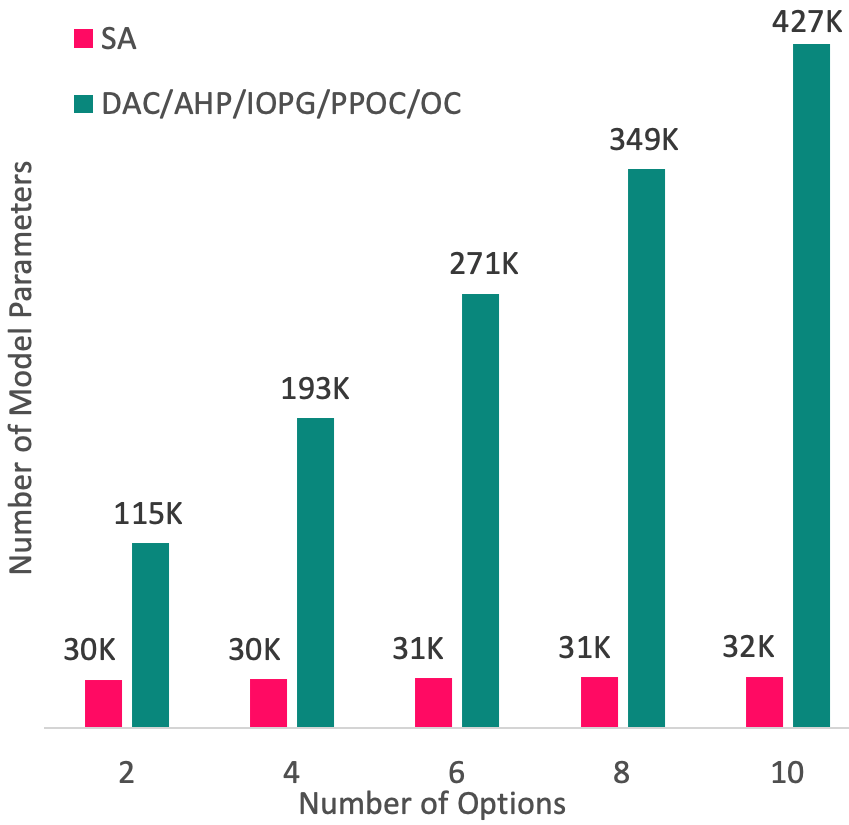
\includegraphics[width=1\linewidth]{figures/scale.png}
%   \caption{\label{fig:sa_scale} Model Scale Comparison.}
%   \vspace{-5mm}
% \end{wrapfigure}

The option framework \cite{sutton1999between} is one of the most
promising framework to extend RL methods to lifelong learning
agents \cite{mankowitz2016adaptive} and has been proved
beneficial in speeding learning~\cite{bacon2018temporal},
improving exploration \cite{harb2018waiting}, and facilitating
transfer learning \cite{zhang2019dac}. However, conventional
options tend to over-complicate methods in ways that are less
suited to leveraging computation \cite{bacon2018temporal}.

The first deficiency is that the option framework is developed on
Semi-Markov Decision Process, we refer to this as
\emph{SMDP-Option}. In \emph{SMDP-Option}, an option is a
temporally abstracted action whose execution cross a various
amount of time steps. \emph{SMDP-Option} has been identified
\cite{zhang2019dac} as sample inefficient and unstable to
optimize. Since RL is notoriously sample expensive and
hyper-parameters sensitive \cite{haarnoja2018soft}, the SMDP
formulation severely impair options' applicability in broader
context \cite{jong2008utility}.

We address this issue by first proving that \emph{SMDP-Option}
has a sample efficient Markov Decision Process equivalence
(\emph{bisimulation relation} \cite{givan2003equivalence}), we
refer to this as \emph{MDP-Option}. In RL
\cite{levy2011unified,zhang2019dac} and Imitation Learning
\cite{henderson2018optiongan,sharma2018directed,shankar2020learning,lee2020learning}
areas, similar formulations have been employed as ``one-step
option'' \cite{henderson2018optiongan,zhang2019dac}, such
approximations either drop the dependency on $\rvo_{t-1}$ (option
executed from last steps) thus lose the temporal abstraction
functionality, or use an inaccurate value function to update
policies. Instead, we are the first identify the issue that the
conventional \emph{Value Function} $V[\rvs_t]$ no longer yields
the Bellman equation \cite{sutton1999between} under the one-step
setting, and preserve the temporal abstraction by proposing a
novel \emph{Markovian Option-Value Function}
$\bar{V}[\rs_t,\rvo_{t-1}]$, which is an unbiased estimation of
$V[\rs_t]$ and its variance is up-bounded by $V[\rs_t]$, and
derive the novel Bellman equation for \emph{MDP-Option}. Based on
the Bellman equation, we not only prove the equivalence to
\emph{SMDP-Option}, but also derive policy gradient theorems for
learning \emph{MDP-Option}. As a result, \emph{MDP-Option} is a
general-purpose MDP which can be combined with any MDP-style
\cite{zhang2019dac} policy optimization algorithms (such as PPO
\cite{witoonchart2017application}) off-the-shelf.

The second deficiency of \emph{SMDP-Option} is that it is
extremely expensive to learn and scale up. Each option is
represented as a triple containing three components: one
\emph{intra-option policy}, one \emph{termination function}, and
one initiation set. Learning options is amenable to learning
local representations \cite{bacon2018temporal} on a statistical
manifold \cite{amari1987differential}. As pointed out by
\citename{bacon2018temporal} (Chapter 3.6), local representations
do a poor job at representing knowledge compactly and require
more samples than distributed representations.

In this paper, we make the first attempt to learn options with
embeddings (distributed representations
\cite{hinton1986learning}). Distributed representations have
proved its efficacy in representing entities and played a central
role in recent advances of large-scale frameworks in both CV
\cite{krizhevsky2012imagenet,dosovitskiy2020image} and NLP
\cite{vaswani2017attention,devlin2018bert,brown2020language}
areas. As shown in Section \ref{sec:net_arch}, \emph{MDP-Option}
naturally gives rise to representing each option as a single
embedding vector and the option space as an ambient space of the
state space. Therefore, options defined in \emph{MDP-Option}
combine temporal abstraction together with state abstraction
\cite{knoblock1990learning}. To learn option embeddings, we
propose \emph{Option2Vec} (O2V) architecture, a simple yet
effective Attention \cite{vaswani2017attention} based
Encoder-Decoder architecture. Complexities of learning option
distributions and classification hyperplanes on statistical
manifold are simplified as an efficient clustering mechanism over
option embedding centroids on a homeomorphic parametric space
\cite{amari1987differential}. We illustrate this difference
between \emph{SMDP-Option} and \emph{MDP-Option} in Figure
\ref{fig:o2v_manifold}.
\begin{figure*}[h!]
  \vspace{-4mm} \centering
  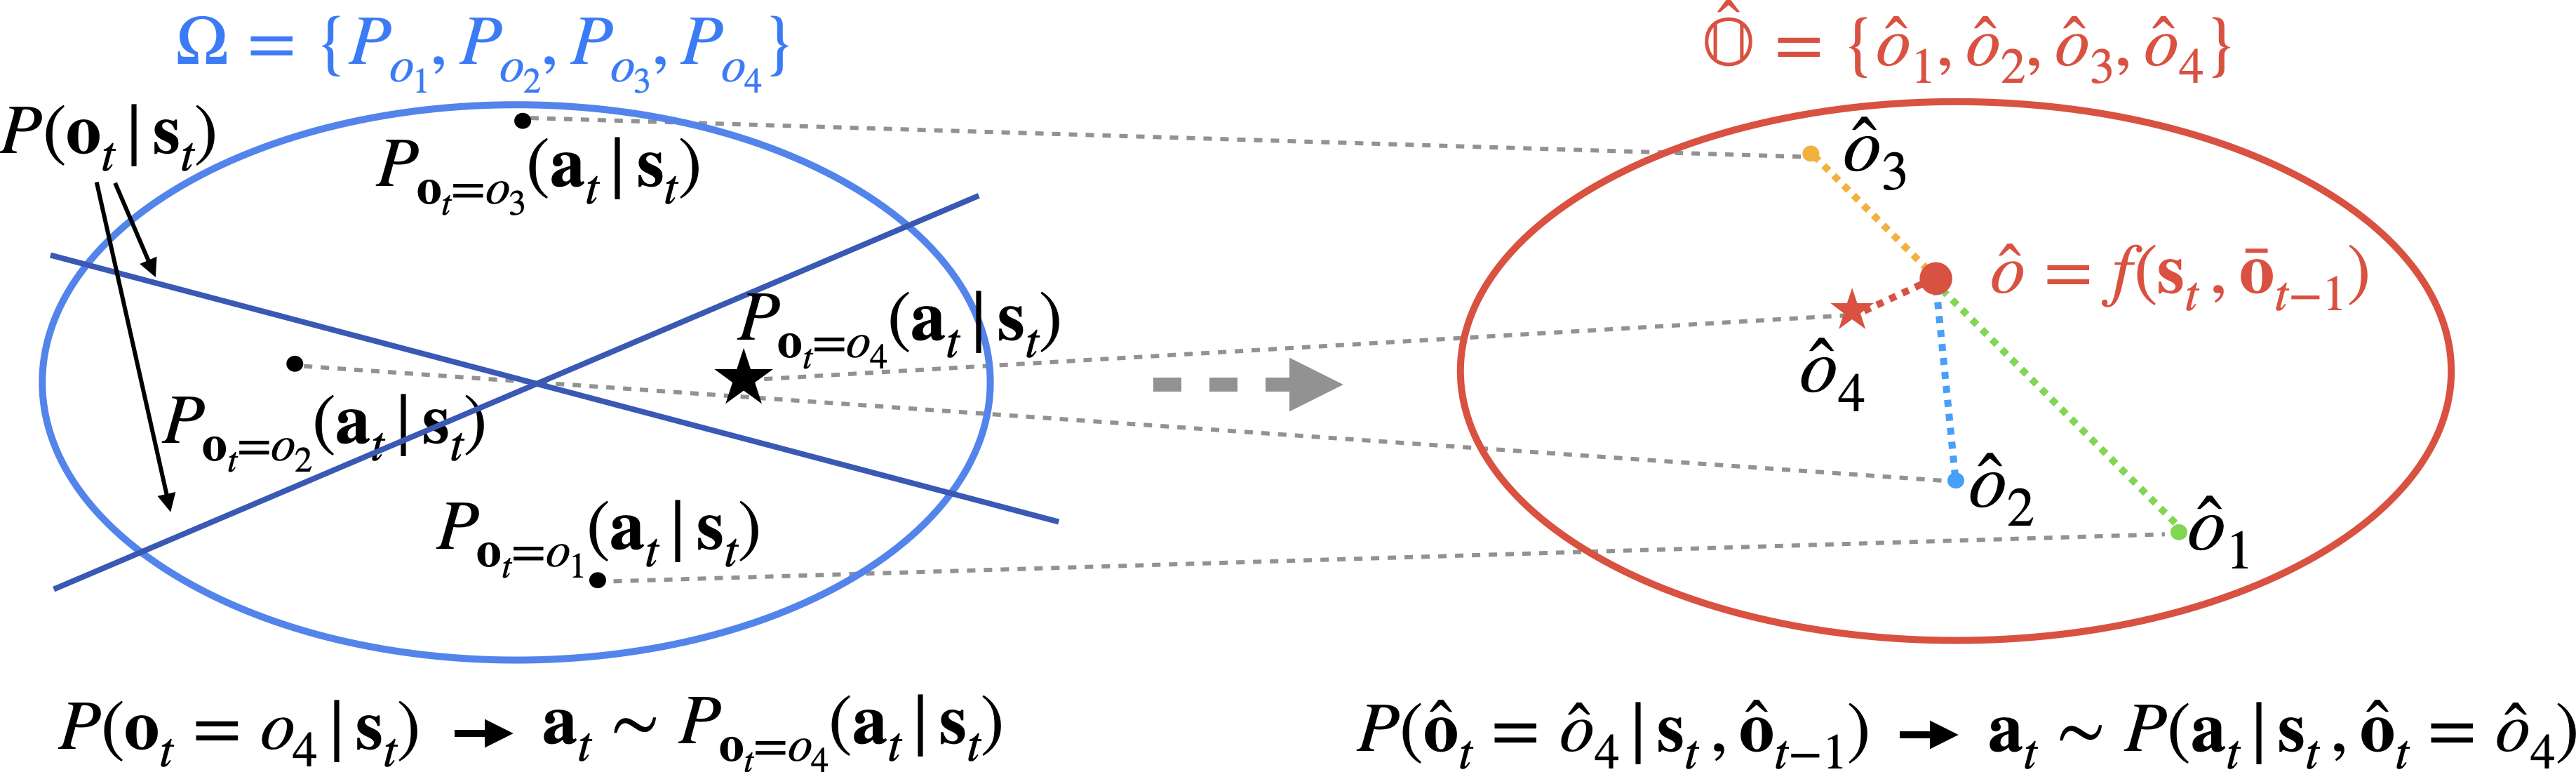
\includegraphics[width=0.9\linewidth]{figures/O2V_Manifold.png}\\
  \vspace{-1mm} \centering
  \caption{\label{fig:o2v_manifold} Illustrations of
    \blue{\emph{SMDP-Option} Classification} on \blue{Statistical
      Manifold} v.s. \red{\emph{MDP-Option} Clustering} on
    \red{Parametric Space}. On Statistical Manifold, for $M$
    options there are \blue{$M$ action policies} to learn.
    Selecting options is analogously \blue{learning
      classification hyperplanes}. On Parametric Space, for $M$
    options there are \red{$M$ embedding centroids} to learn yet
    all embeddings \red{share a single action policy (decoder)}.
    Selecting options is analogously \red{assigning the closest
      centroid to the hyperplace $[\rvs_t,\rvo_{t-1}]$}.}
  \vspace{-5.5mm}
\end{figure*}

It is worth to point out that, due to space limitation we have to
solely focus on proposing \emph{MDP-Option} and O2V, and
designing experiments to address that O2V achieves at least the
same performance as \emph{SMDP-Option}. Since \emph{MDP-Option}
is equivalent to \emph{SMDP-Option}, it still shares many
identified limitations such as ``the dominant skill problem''
\cite{vezhnevets2017feudal,zhang2019dac} as identified in Section
\ref{sec:exp_ext}. As briefly discussed in Appendix
\ref{sec:append_gist}, \emph{MDP-Option} actually gives rise to
efficient solutions to many identified limitations of
\emph{SMDP-Option} yet have to be deferred to our future works.
Our main contributions are: (1) proposing the \emph{MDP-Option},
a MDP equivalence of \emph{SMDP-Option}, and developing the
bellman equation and gradient theorems; (2) proposing option
embedding vectors, the first distributed representations of
options; (3) proposing the first Attention
\cite{vaswani2017attention} based Encoder-Decoder architecture,
the Option2Vec (O2V) architecture, for learning options with much
better scalability, smaller variance and faster convergence; (4)
demonstrating option embeddings are interpretable, which is a key
property for developing real-world RL applications (e.g. ensuring
safety for human).

% A better way to employ large scale computability. treated as
% undirected graph. learn dependencies end-to-end manner.
% interpretability; safety

% To the best of our knowledge, MDP-Skill is the first MDP enables
% distributed representations of temporal abstractions. O2V is the
% first embedding, attention and encoder-decoder.

% skill embedding can be seen as a minimal (amy zhang iclr2021)
% causal set describing temporal-state (dynamic aware) irrelevant
% by adding extra in objective (feudal net).

% As explained in Appendix \ref{sec:appen_gist}, first-order markov
% formulated MDP-Skill did not fully exploit the potential of O2V. a
% Deep (multi-hierarchy) Wide (higher-order) MDP-Skill will fully
% unleash the power of O2V and gives rise to a general-purpose
% large-scale pre-training framework in RL. We focus this work on
% proposing MDP-Skill and O2V and will explore DWO2V in the future
% work.

% % \item Large variance
% %   \cite{zhang2019dac,haarnoja2018soft}: SMDP
% %   algorithms are notoriously sensitive to hyperparameters . Due
% %   to the SMDP formulation, more stable Markov Decision Process
% %   (MDP) policy gradient algorithms cannot be used.

% % \begin{enumerate}
% % \item O2V is more sample efficient, because a) O2V is MDP
% %   formulated, thus sample at each time step can be used to update
% %   the skill policy; and b) Only one action policy decoder is
% %   needed. It learns to decode each dimension of the skill context
% %   vector at each time step whichever skill is activated;
% % \item O2V has smaller variance, because a) The skill value upon
% %   arrival function (Eq.~(\ref{eq:sa_v})) is theoretically and
% %   empirically proven to have smaller variance than the
% %   conventional value function; and b) O2V only needs to train two
% %   (skill and action) policy networks; and c) O2V can employ more
% %   stable MDP based policy gradient algorithms (e.g.
% %   PPO~\cite{schulman2017proximal});
% % \item O2V has better scalability, because a) Regardless of the
% %   number of skills, only two policies need to be trained; and b)
% %   Adding one more skill is as cheap as adding a context vector;
% %   % to write: disentangle; exploration; convergence speed;
% %   % interpretability; generalization
% % \item O2V is more effective, because a) On infinite-horizon
% %   environments, O2V significantly outperforms the other models;
% %   and b) On transfer learning environments, O2V ranks the first in
% %   5 out of 6 environments and shows its advantages in knowledge
% %   reuse tasks;
% % \item O2V has better interpretability. Unlike the option framework
% %   encodes abstract knowledge implicitly in action policies,
% %   knowledge of a skill is explicitly encoded in each dimension of
% %   the skill context vector.
% % \end{enumerate}


% % % Incomplete Ideas:

% % % 1. 问问题,要解决什么问题,在干什么
% % % 2. 当前sota什么状况,但是有什么问题
% % % 3. 你做了啥,为啥能解决问题
% % % 4. 你这东西有啥特点
% % % 5. 怎么证明这东西work
% % % 6. Implication 是啥

% % % to write: smaller variance
% % % to write: only one critic
% % % to write: deep large scale; imitation; causual relationship
% % % because each run variance so small; not only exploration.

% % % todo: skill not pg/bp; may be dynamic routing/inference/K-means
% % % is enough. should have much simpler design

% % % todo: why option converges slower than action? disentangle paper

% % % todo: supervised train O2V first -> reinf train O2V; Imitation
% % % Learning (dm-control CMU humanoid-v3)

% % % todo: formal def of the turkey: latent variables between
% % % actions and environment. Not observable but truly exists
% % % ; design an experiment to show this problem

% % % potential problem: currently p(o_t|s_t,o_{t-1}) is updated
% % % using Q(o_t,s_t). Should it be Q(o_t,s_t,o_{t-1})? Should
% % % R_{t+1} depends on o_{t-1}?

% % % Yes it should. Reason:

% % % No it should not. Reason: We should not model environment. This
% % % is model free algo. Even though in reality, environment depends
% % % on latent variable $o_{t-1}$ to give R_{t+1}. But we should not
% % % model this relationship in Q value.
% % % Problem: Q used to update p(o'|s',o) does not consider o
% % % Possible solution: instead of include o in Q, create another
% % % ``latent variable environment reward mechanism'' function.
% % % Explicitly model this latent relationship between skill and
% % % environment's reward

% % % A state-previous-skill pair.
% % % Previous research only consider abstract, did not demonstrate
% % % contextual information. Knowing which action has been done can
% % % help predicting whats the next move. Cooking example
% % % Temporal relationships between skills (skill context) has not
% % % been explored before. Seems to encode only one-step temporal
% % % relationship. In order to encode multi time steps relationships,
% % % one can use longer history by turning into higher order markov,
% % % but still markov. our proof still holds. (e.g. adding temporal
% % % masks back to attention, extending the decoder input vector to a
% % % matrix, where rows are time steps, turn it into a k-order markov
% % % process). Remain open for future work.

% % % todo: explain why attention is not the best

% % % idea: In order to have better temporal representation what has
% % % happened before, need a dynamic routing like forward algorithm
% % % to encode all skills have been taken in time series

% % % idea: maximizing reasoning entropy
% % % statistical random variables decreasing bias increasing variance
% % % reasoning variables decreasing bias decreasing variance;
% % % maximizing reasoning entropy

% % % todo: MDP equi minor contribution
% % % todo: Equations addressed stuffed turkey (skill policy, decoder
% % % in nn)
% % % todo: reasons for oc -> sa based on MDP:

% % % minor contribution: MDP
% % % straight forward extend to deeper layer
% % % NLP interface to understand/instruct which dimension encode
% % % what information

\section{Background}
\label{sec:smdp_option}

\textbf{Markov Decision Process:} A Markov Decision Process
\cite{puterman2014markov} $M=\{\sS,\sA,R,P,\gamma\}$ consists of
a state space $\sS$, an action space $\sA$, a state transition
function $P(\rvs_{t+1}|\rvs_t,\rva_t):
\sS\times\sA\rightarrow\sS$, a discount factor $\gamma\in\sR$,
and a reward function
$R(\rvs,\rva)=\E[r|\rvs,\rva]:\sS\times\sA\rightarrow\sR$ which
is the expectation of the reward $r_{t+1}\in\sR$ received from
the environment after executing action $\rva_t$ at state
$\rvs_t$. A policy
$\pi=P(\rva|\rvs):\sA\times\sS\rightarrow[0,1]$ is a probability
distribution defined over actions conditioning on states. A
discounted return is defined as $G_t =
\sum_k^N\gamma^kr_{t+k+1}$, where $\gamma\in (0,1)$ is a
discounting factor. The value function
$V[\rvs_t]=\E_{\tau\sim\pi}[G_t|\rvs_t]$ is the expected return
starting at state $\rvs_t$ and the trajectory
$\tau=\{\rvs_t,\rva_t,r_{t+1},\rvs_{t+1},\dots\}$ follows policy
$\pi$ thereafter. The action-value function is defined as
$Q[\rvs_t,\rva_t]= \E_{\tau\sim\pi}[G_t|\rvs_t,\rva_t]$.

\textbf{Bisimulation Relation:} Given two processes
$M=\{\sS,\sA,R,P,\gamma\}$ with the trajectory $\tau$ and
$\tilde{M}=\{\tilde{\sS},\sA,\tilde{R},\tilde{P},\tilde{\gamma}\}$
with the trajectory $\tilde{\tau}$. Assume both $M$ and
$\tilde{M}$ share the same action space $\sA$. The equivalence
relation between $M$ and $\tilde{M}$ is defined by
\citename{givan2003equivalence}. An equivalence relation
$\tilde{B}:\tilde{\sS}\rightarrow\sS$ is a \emph{Bisimulation
  Relation} if 1) for any state $\rvs$, there exists an
\emph{one-to-one correspondence} equivalent state $\tilde{\rvs}$
that $\rvs/\tilde{B}=\tilde{\rvs}/\tilde{B}$, or denoted as
$\tilde{B}(\tilde{\rvs})=\rvs$, 2) and the following conditions
hold:
\begin{enumerate}
  \label{def:bisimulate}
\item
  $\;\;\;\;\;\;\;\;\;\;\;\;\;\;\;\;\;\;\;\;\;\;$$P(\tau/\tilde{B})\equiv
  P(\tilde{\tau}/\tilde{B}),\;\;\;
  \text{and\;}\tilde{B} \text{\;is a \emph{bijection}},$\\
\item
  $\;\;\;\;\;\;\;\;\;\;\;\;\;\;\;\;\;\;\;\;\;\;$$V[\tau/\tilde{B}]\equiv
  V[\tilde{\tau}/\tilde{B}]$
\end{enumerate}

In this paper, we follow this definition to prove the equivalence
relationship.

\textbf{The SMDP-based Option Framework}: In \emph{SMDP-Option}
\cite{sutton1999between,bacon2018temporal}, an option is a triple
$(\sI_o, \pi_o, \beta_o)\in \gO$, where $\gO$ denotes the option
set; the subscript $o\in\sO=\{1,2,\dots,K\}$ is a positive
integer index which denotes the $o$th triple where $K$ is the
number of options; $\sI_o$ is an initiation set indicating where
the option can be initiated;
$\pi_o=P_o(\rva|\rvs):\sA\times\sS\rightarrow[0,1]$ is the action
policy of the $o$th option;
$\beta_o=P_o(\rvb=1|\rvs):\sS\rightarrow[0,1]$ where $\rvb\in
{0,1}$ is a \emph{termination function}. For clarity reasons, we
use $P_o(\rvb=1|\rvs)$ instead of $\beta_o$ which is widely used
in previous option literatures (e.g.
\cite{sutton1999between,bacon2017option}).

A \emph{master policy} $\pi(\rvo|\rvs)=P(\rvo|\rvs)$ where
$\rvo\in\sO$ is used to sample which option will be executed.
Note that we use the bold-case $\rvo$ to denote unrealized random
variables and the light-italic-case $o$ to denote a realized
instantiation. Conventionally, the execution of an option employs
the call-and-return model \cite{sutton1999between}: at time step
$t$, an agent either continues the previously executed option
$\rvo_{t-1}=o$ with probability $P_o(\rvb=0|\rvs)$ and sets
$\rvo_t=\rvo_{t-1}=o$, or terminates $o$ with probability
$P_o(\rvb=1|\rvs)$ and samples a new option $\rvo_t$ from the
master policy $P(\rvo_t|\rvs_t)$. Therefore, the dynamics
(stochastic process) of the option framework is written as:
\begin{align}
  \label{eq:oc_pgm_joint}
  P(\tau) = P(\rvs_0)&P(\rvo_0)P_{o_0}(\rva_0|\rvs_0)\prod_{t=1}^\infty P(\rvs_t|\rvs_{t-1},\rva_{t-1})P_{o_t}(\rva_{t}|\rvs_{t})\nonumber\\
                     &[P_{o_{t-1}}(\rvb_t=0|\rvs_t)\1_{\rvo_t=o_{t-1}} +P_{o_{t-1}}(\rvb_t=1|\rvs_t)P(\rvo_t|\rvs_t)].
\end{align}
where $\tau=\{\rvs_0,\rvo_0,\rva_0,\rvs_1,\rvo_1,\rva_1,\ldots\}$
denotes the trajectory of the option framework. $\1$ is an
indicator function and is only true when $\rvo_t=o_{t-1}$ (notice
that $o_{t-1}$ is the realization at $\rvo_{t-1}$). Therefore,
under this formulation the option framework is defined as a
Semi-Markov process since the dependency on an activated option
$o$ can cross a variable amount of time \cite{sutton1999between}.
% For the clarity and page limitation, it is enough to only focus
% on the underlying stochastic processes as marginalized versions
% of decision processes in this paper. The complete decision
% process is deferred in Appendix \ref{sec:appen_oc_pgm}.

\section{MDP Equivalences of the SMDP-based Option Framework}
\label{sec:smdp_mdp_sa}
We prove that \emph{MDP-Option} is equivalent to
\emph{SMDP-Option} under the definition of \emph{bisimulation}
\cite{givan2003equivalence}. To derive Bellman equation for
\emph{MDP-Option}, we develop a novel \emph{Markovian skill-value
  function} $\bar{V}[\rvs_t,\rvo_t]$, which is an unbiased
estimation of the conventional value function $V[\rvs_t]$ and the
variance of $\bar{V}[\rvs_t,\rvo_t]$ is up-bounded by
$V[\rvs_t]$. Based on Bellman equation, policy gradient theorems
for \emph{MDP-Option} are then derived. As a result,
\emph{MDP-Option} is a general-purpose MDP which can be combined
with any policy optimization algorithm off-the-shelf.


In this section, we propose \emph{MDP-Option}, a simple yet
effective option-induced MDP and prove its equivalence (as shown
in Figure \ref{fig:sa_logic}) to \emph{SMDP-Option}. For clarity,
in Section \ref{sec:mdp_option} we first prove an intermediate
equivalence \emph{MDP-Mixture} to bridge the equivalence between
\emph{SMDP-Option} and \emph{MDP-Option}. Based on
\emph{MDP-Mixture}, in Section~\ref{sec:sa_PGM} we propose the
\emph{MDP-Option}, a marginalized variation of the \emph{SMDP-Option}. \emph{MDP-Option}
uses the \emph{skill policy} (Eq.~\ref{eq:sa_pgm_joint}), which
is a marginal distribution, to replace the \emph{master policy}
and \emph{termination function}. In order to derive \emph{MDP-Option}'s
Bellman equation, we propose the novel \emph{Markovian
  skill-value function} (Eq.~\ref{eq:sa_v}) and prove that it is
an unbiased estimation of the conventional value function and its
variance is up-bounded by the conventional value function. Policy
gradient theorems for \emph{MDP-Option} are then derived basing on the
Bellman equation. In Section~\ref{sec:net_arch}, we propose O2V,
which is an implementation of the \emph{MDP-Option} by employing the
Embedding and Attention \cite{vaswani2017attention} techniques.
\begin{figure*}[h!]
  \vspace{-4mm} \centering
  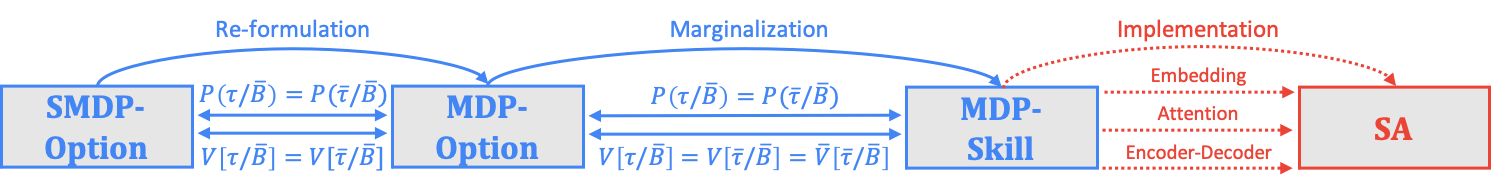
\includegraphics[width=1\linewidth]{figures/SA_Logics.png}\\
  \caption{\label{fig:sa_logic} \red{Paper Structure?}.
    \blue{Blue} terms are \blue{Decision Processes}. Solid arrows
    indicate that their equivalences are theoretically justified.
    \red{O2V} is an \red{Architecture} which implements the
    \blue{MDP-Option} by employing Embedding, Attention, and
    Encoder-Decoder techniques. Dashed connections indicate they
    are architecture choices.}
\vspace{-5.5mm}
\end{figure*}

% to implement the temporal extension by employing the attention
% mechanism~\cite{vaswani2017attention}. describes the dynamics
% (Markov process) of O2V. Section~\ref{sec:sa_mdp} defines value
% functions on top of the dynamics, thus formulating the MDP.
% Policy gradient theorems are then derived.
% Section~\ref{sec:net_arch} implements O2V by employing neural
% networks and the Multi-Head Attention
% mechanism~\cite{vaswani2017attention}, which enables O2V to
% temporally extend skills in the absence of the termination
% function.


\subsection{The MDP Equivalence (MDP-Mixture) of the Option
  Framework}
\label{sec:mdp_option}
With the definitions of \emph{SMDP-Option} in hand, we now show
how to reformulate it into an MDP-based equivalence
\emph{MDP-Mixture}. The first reformulation is that we follow
\citename{bishop2006pattern}'s formulation of mixture
distributions and redefine the option random variable
$\rvo\in\sO=\{1,2,\dots,K\}$, which was originally defined as an
integer index, but now as a $K$-dimensional one-hot vector
$\bar{\rvo}\in\bar{\sO}=\{0,1\}^K$ where $K$ is the number of
options. The second reformulation is that we exploit the one-hot
vector to reformulate the \emph{termination function} and action
function of each option into two mixture distributions by
introducing extra dependencies on $\bar{\rvo}$:
\begin{align}
  \label{eq:mdp_action_termination}
P(\rva_t|\rvs_t,\bar{\rvo}_t) =
\prod_{o\in\bar{\rvo}_t}P_{o}(\rva_t|\rvs_t)^{o},\;\;\;\;\;\;\;\;\;
P(\rvb_t|\rvs_t,\bar{\rvo}_{t-1}) =
\prod_{o\in\bar{\rvo}_{t-1}}P_{o}(\rb_t|\rvs_t)^{o}
\end{align}
Since the option random variable $\bar{\rvo}$ is now a one-hot
vector, for $\bar{\rvo}_t=o_t$, by definition only the entry
$o_t=1$ and all the other entry $o\in\sO-\{o_t\}=0$. Therefore,
we have
$P_{o_t}(\rva_t|\rvs_t)=P(\rva_t|\rvs_t,\bar{\rvo}_t=o_t)$ and
$\beta_{o_{t-1}}=P_{o_{t-1}}(\rvb_t=1|\rvs_t)=P(\rvb_t=1|\rvs_t,\bar{\rvo}_{t-1}=o_{t-1})$.

The third reformulation is that we propose a novel \emph{MDP
  mixture master policy}
$P(\bar{\rvo}_t|\rvs_t,\rvb_t,\bar{\rvo}_{t-1})$, which is a
mixture distribution containing the \emph{SMDP master policy} and
a degenerate probability as mixture components by adding two
extra dependencies on $\rvb_t$ and $\bar{\rvo}_{t-1}$:
\begin{equation}
  \label{eq:mdp_oc_po}
P(\bar{\rvo}_t|\rvs_t,\rvb_t,\bar{\rvo}_{t-1}) = P(\bar{\rvo}_t|\rvs_t)^{\rb_t}P(\bar{\rvo}_t|\bar{\rvo}_{t-1})^{1-\rb_t},
\end{equation}
where the indicator function $\1_{\rvo_t=o_{t-1}}$ used in
Eq.\ref{eq:oc_pgm_joint} is now redefined as a degenerate
probability distribution~\cite{puterman2014markov}:
\begin{equation*}
  \label{eq:deg_puterman}
P(\bar{\rvo}_t|\bar{\rvo}_{t-1}) = 
\begin{cases}
  1&\;\text{if } \bar{\rvo}_t=\bar{\rvo}_{t-1},\\
  0&\;\text{if } \bar{\rvo}_t\neq\bar{\rvo}_{t-1}.
\end{cases}
\end{equation*}

We define a function
$\bar{B}(\bar{\rvo})=\bar{\rvo}\cdot\rvd^T:\bar{\sO}\rightarrow\sO$
which maps $\bar{\rvo}$ to $\rvo$, where $\rvd=[1,2,\dots,K]^T$
is a $K$-dimensional constant integer vector and hence
$\bar{B}(\bar{\rvo})=\rvo$. Note that $\bar{B}$ is a
\emph{Bijection} since it is a linear function defined on a
finite integer space. Therefore, by following the definition of
\emph{Bisimulation Relation}, the dynamics of the \emph{SMDP-Option} in
Eq.\ref{eq:oc_pgm_joint} under the Bijection $\bar{B}$ can be
reformulated as:
\begin{align}
  \label{eq:mdp_pgm_joint}
  P(\tau/\bar{B}) = P(\bar{\tau}/\bar{B}) = P(\rvs_0)&P(\bar{\rvo}_0)P(\rva_0|\rvs_0,\bar{\rvo}_0)\prod_{t=1}^\infty P(\rvs_t|\rvs_{t-1},\rva_{t-1})P(\rva_{t}|\rvs_{t},\bar{\rvo}_{t})\nonumber\\
                                                     &\sum_{\rvb_t}P(\rvb_t|\rvs_t,\bar{\rvo}_{t-1})P(\bar{\rvo}_t|\rvb_t,\rvs_t,\bar{\rvo}_{t-1})
\end{align}
where
$\bar{\tau}=\{\rvs_0,\bar{\rvo}_0,\rva_0,\rvs_1,\bar{\rvo}_1,\rva_1,\ldots\}$
is the trajectory of the \emph{MDP-Mixture}.
% Notice that under this formulation, $P(\tau)$ is actually an
% HMM with $\rvs_t$, $\rva_t$ as observable random variables and
% $\rvb_t$, $\bar{\rvo}_t$ as latent variables.

With $P(\tau/\bar{B}) = P(\bar{\tau}/\bar{B})$ in hand, to prove the
equivalence between the \emph{SMDP-Option} and \emph{MDP-Mixture}, we move on to
prove both of them share the same expected reward. This is
non-trivial since compared to the \emph{SMDP-Option}, the MDP
formulation introduces extra dependencies on $\bar{\rvo}$ and
$\rvb$ in Eq.\ref{eq:mdp_pgm_joint} as described above. However,
in Appendix \ref{sec:appen_mdp}, by exploiting conditional
independencies we prove that they do have the same expected
return under the Bijection $\bar{B}$. Therefore, the SMDP-based
option framework has an MDP-based equivalence:
\begin{thm}
  \label{theo:smdp_mdp}
  By the definition of Bisimulation Relation, the SMDP-based
  option framework, which employs Markovian options, has an
  underlying MDP equivalence because:
\end{thm}
\begin{enumerate}
\item
  $\;\;\;\;\;\;\;\;\;\;\;\;\;\;\;\;\;\;\;\;\;\;$$P(\tau/\bar{B})
  = P(\bar{\tau}/\bar{B})$
  (Eq. \ref{eq:mdp_pgm_joint}) and $\bar{B}$ is a Bijection.\\
\item
  $\;\;\;\;\;\;\;\;\;\;\;\;\;\;\;\;\;\;\;\;\;\;$$V[\tau/\bar{B}]=V[\bar{\tau}/\bar{B}]$
  (Proofs in Appendix \ref{sec:appen_mdp}).
\end{enumerate}

\subsection{The Option2Vec induced Markov Decision Problem
  (MDP-Skill)}
\label{sec:sa_PGM}

\begin{wrapfigure}{r}[1pt]{0.4\textwidth}
  \vspace{-4mm}
  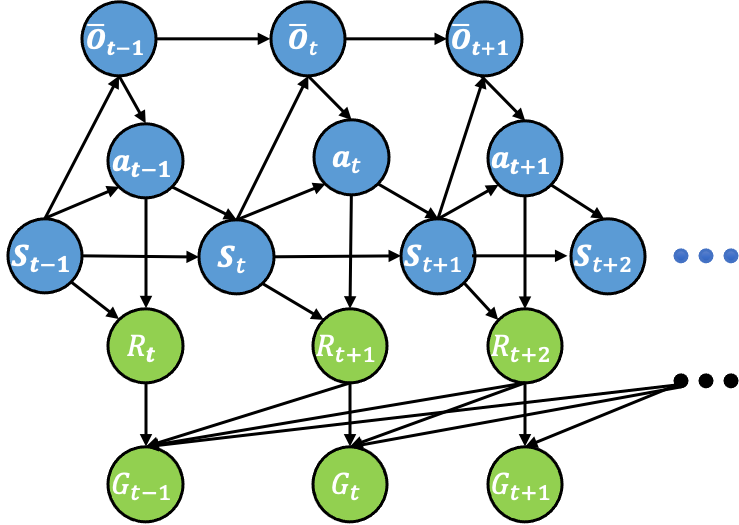
\includegraphics[width=1\linewidth]{./figures/doe.png}
  \caption{\label{fig:pgm_mdp_skill} Graphical Model of
    \emph{MDP-Option}}
  \vspace{-5mm}
\end{wrapfigure}

% \begin{figure*}[thb]
%   \centering
%   \begin{tabular}{cc}
%     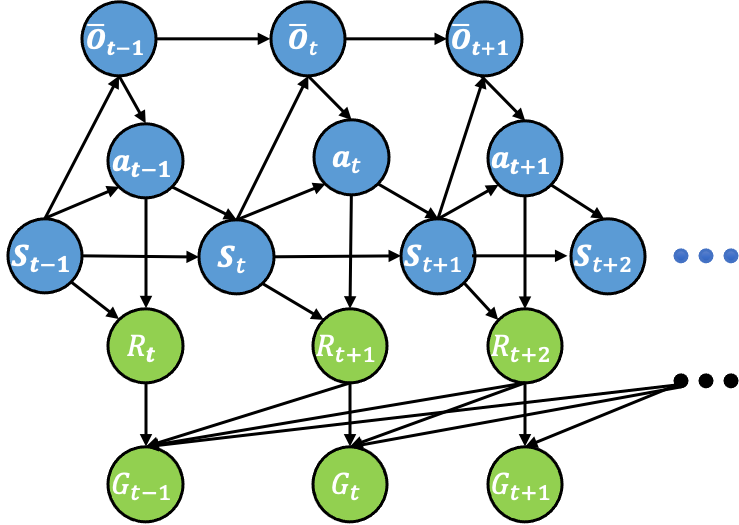
\includegraphics[width=0.45\linewidth]{./figures/doe.png}&
%                                                                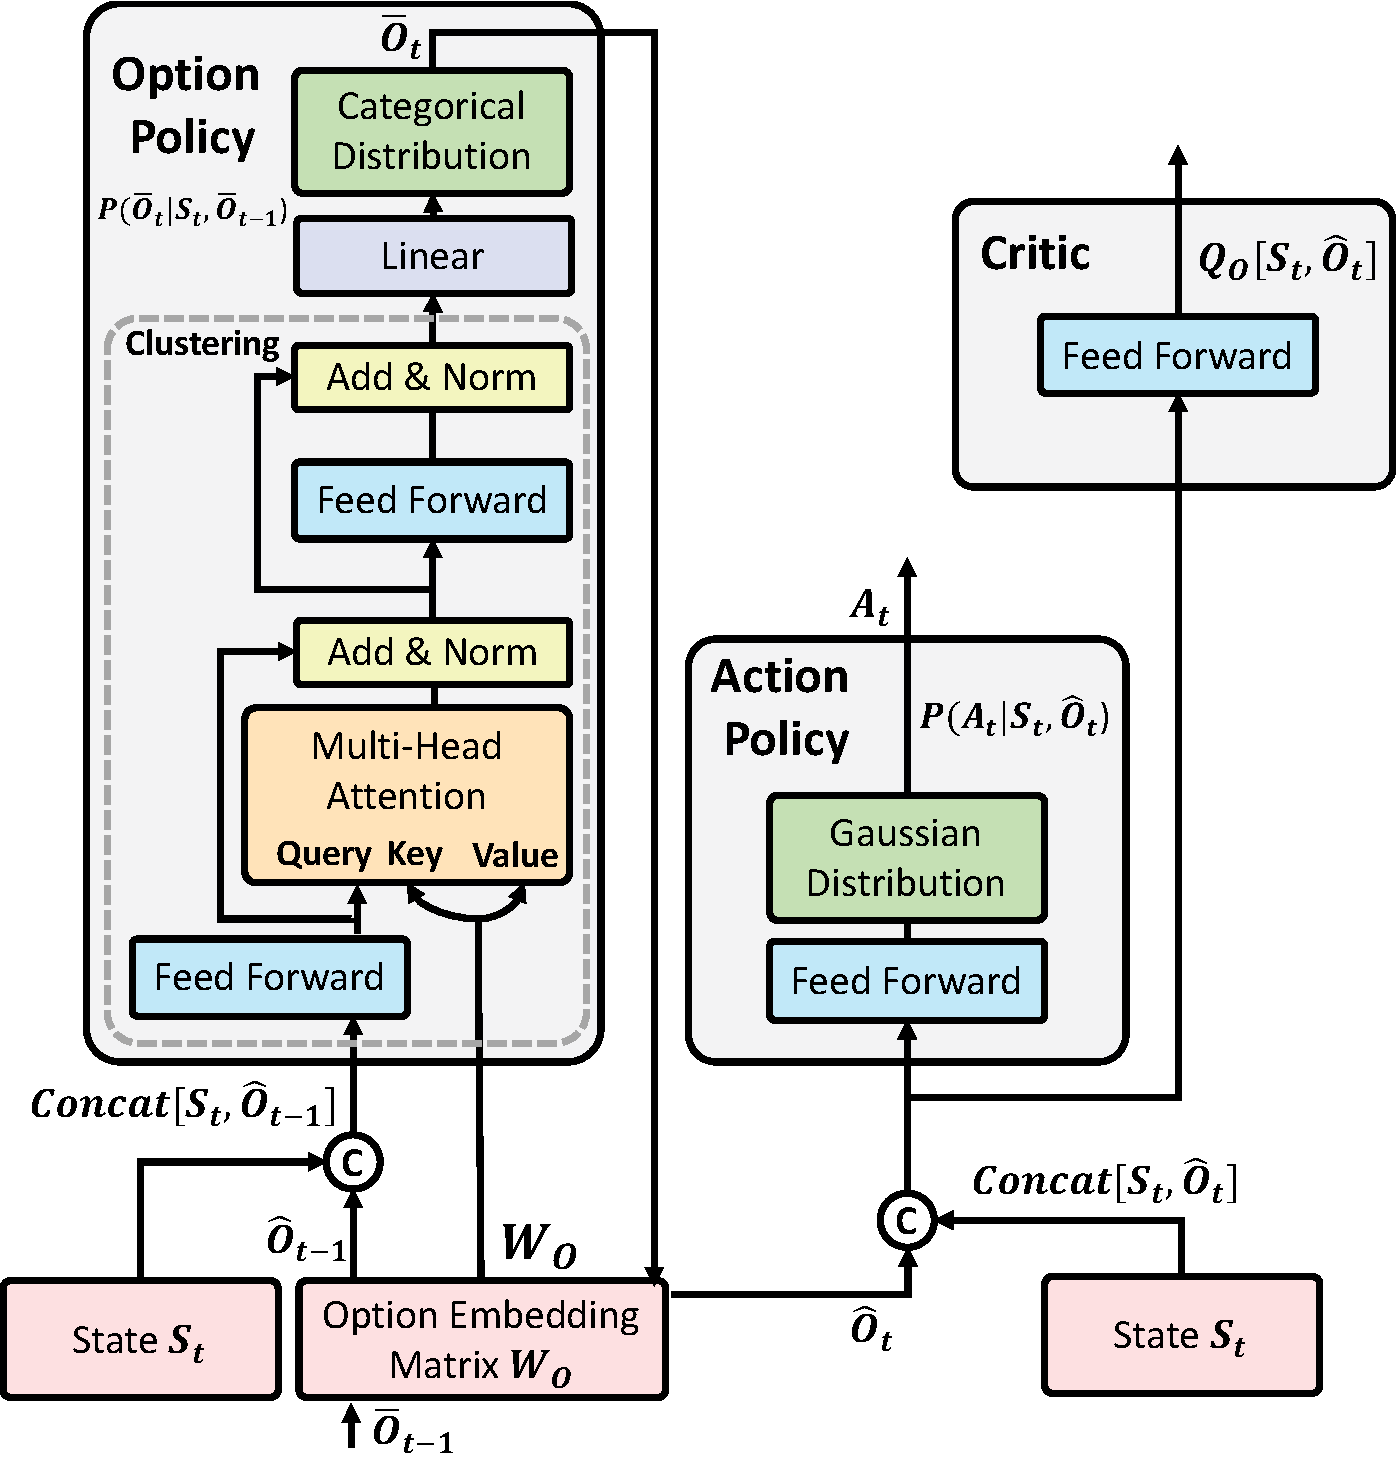
\includegraphics[width=0.45\linewidth]{./figures/sa_attn_net.png}\\
%     {\small (a) Graphical Model of the MDP-Skill}&
%                                                 {\small (b) The Option2Vec Architecture (SA)}\\
   
%   \end{tabular}\vspace{-2mm}
%   \caption{\label{fig:sa_net} O2V is a Neural Network
%     implementation of the MDP-Skill}
% \end{figure*}

In this section, we define the option-induced MDP,
\emph{MDP-Option}, prove the equivalence between \emph{MDP-Option}
and \emph{SMDP-Option}, and derive policy gradient theorems for
\emph{MDP-Option}. Although the mixture master policy in
Eq.\ref{eq:mdp_pgm_joint} is MDP-formulated, the master policy
$P(\bar{\rvo}_t|\rvs_t)$ as a mixture component in it is still
SMDP-formulated hence cannot be updated by MDP-based algorithms.
The beauty of \emph{MDP-Option} is that it addresses this issue in a
natural and simple way: notice the marginalization over the
termination variable $\rvb_t$ in Eq. \ref{eq:mdp_pgm_joint}:
$\sum_{\rvb_t}P(\rvb_t|\rvs_t,\bar{\rvo}_{t-1})P(\bar{\rvo}_t|\rvb_t,\rvs_t,\bar{\rvo}_{t-1})$,
\emph{MDP-Option} uses the \emph{skill policy}
$P(\bar{\rvo}_t|\rvs_t,\bar{\rvo}_{t-1})$ to model this marginal
distribution explicitly:
\begin{align}
  \label{eq:sa_pgm_joint}
  P(\bar{\tau})=P(\rvs_0)P(\bar{\rvo}_0)P(\rva_0|\rvs_0,\bar{\rvo}_0)
  \prod_{t=1}^\infty P(\rvs_t|\rvs_{t-1},\rva_{t-1})
  P(\rva_{t}|\rvs_{t},\bar{\rvo}_{t})P(\bar{\rvo}_t|\rvs_t,\bar{\rvo}_{t-1})
\end{align}
Therefore, \emph{MDP-Option} shares the same trajectory with the \emph{MDP-Mixture}
while the \emph{skill policy} can be updated by any MDP-based
algorithms. It is natural to ask that how \emph{MDP-Option} temporally
extends an option without the \emph{termination function}. In
fact, the \emph{skill policy} captures temporal relationships
between options explicitly: it selects the new option
$\bar{\rvo}_t$ by choosing the one which has the closest distance
to the current state $\rvs_t$, while has a tendency to continue
the executed option $o$ from the last time step
$\bar{\rvo}_{t-1}=o$. We defer this topic to
Section~\ref{sec:net_arch} and focus this section on proposing
\emph{MDP-Option}.
% denotes the joint distribution of the PGM. Note that under this
% formulation, $P(\tau)$ is actually an Hidden Markov Model (HMM)
% with $\rvs_t$, $\rva_t$ as observable random variables and
% $\hat{\rvo}_t$ as latent variables.

Since the \emph{skill policy}
$P(\bar{\rvo}_t|\rvs_t,\bar{\rvo}_{t-1})$ introduces one extra
dependency on $\bar{\rvo}_{t-1}$, conventional Bellman equation
which is derived by following the conventional value function
$V[\rvs_t]$ no longer applies to \emph{MDP-Option}. In order to derive
the Bellman equation of \emph{MDP-Option}, we propose the novel
\emph{Markovian skill-value function}, value functions with Markov
dependencies (such as $\bar{\rvo}_{t-1}$). Specifically, rather
than use the conventional value function $V[\rvs_t]$, we define
the \emph{Markovian skill-value function} as
$\bar{V}[\rvs_t,\bar{\rvo}_{t-1}]$ (derivations in Appendix
\ref{sec:appen_sa_v_proof}):
\begin{equation}
  \label{eq:sa_v}
  \bar{V}[\rvs_t,\bar{\rvo}_{t-1}]=\E[G_t|\rvs_t,\bar{\rvo}_{t-1}]= \sum_{\bar{\rvo}_t}P(\bar{\rvo}_t|\rvs_t,\bar{\rvo}_{t-1})Q_O[ \rvs_t,\bar{\rvo}_t].
\end{equation}
where the \emph{skill value function}
$Q_O[\rvs_t,\bar{\rvo}_{t}]$ can then be derived as (derivations
in Appendix \ref{sec:appen_sa_v_proof}):
\begin{align}
  Q_O[\rvs_t,\bar{\rvo}_{t}]=\E[G_t|\rvs_t,\bar{\rvo}_{t}]
  \label{eq:sa_q_o}=\sum_{\rva_t}P(\rva_t|\rvs_t,\bar{\rvo}_{t})Q_A[ \rvs_t,\bar{\rvo}_t,\rva_t],
\end{align}
where the \emph{skill-action value function} $Q_A[
\rvs_t,\bar{\rvo}_t,\rva_t]$ can then be derived as (Appendix
\ref{sec:appen_sa_v_proof}):
\begin{align}
\label{eq:sa_q_a}
  Q_A[ \rvs_t,\bar{\rvo}_t,\rva_t]&=\E[G_t| \rvs_t,\bar{\rvo}_t,\rva_t]\nonumber\\
                                  &= r(s,a) + \gamma\sum_{\rvs_{t+1}}P(\rvs_{t+1}|\rvs_t,\rva_t)\bar{V}[\rvs_{t+1},\bar{\rvo}_t],
\end{align}
Expanding $\bar{V}[\rvs_{t+1},\bar{\rvo}_t]$ in
Eq.~\ref{eq:sa_q_a} through Eq.~\ref{eq:sa_v} to \ref{eq:sa_q_a}
gives \emph{MDP-Option}'s Bellman equation. As in
Section~\ref{sec:mdp_option}, we can now move on to prove the
equivalence between the \emph{MDP-Option} and \emph{MDP-Mixture}
hence to \emph{SMDP-Option}. Specifically, in Appendix
\ref{sec:appen_sa_v_proof} we prove that:
\begin{prop}
  \label{prop:var_unb}
  $\bar{V}[\rvs_t,\bar{\rvo}_{t-1} ]$ is an unbiased estimation
  of $V[ \rvs_t ]$.
\end{prop}
Therefore, the SMDP-based option framework and \emph{MDP-Option} are
equivalent under the Bijection $\bar{B}$:
\begin{thm}
  \label{theo:smdp_sa}
  By the definition of Bisimulation Relation, \emph{MDP-Option} is equivalent to
  the SMDP-based option framework because:
\end{thm}
\begin{enumerate}
\item
  $\;\;\;$$P(\tau/\bar{B})=P(\bar{\tau}/\bar{B})$
  (Eq. \ref{eq:mdp_pgm_joint} and \ref{eq:sa_pgm_joint}),\\
\item
  $\;\;\;$$V[\tau/\bar{B}]=V[\bar{\tau}/\bar{B}]\equiv
  \bar{V}[\bar{\tau}/\bar{B}]$ (follows directly from Theorem
  \ref{theo:smdp_mdp} and Proposition \ref{prop:var_unb}).
\end{enumerate}

Other than an unbiased estimation of $V[\rvs_t]$, in Appendix
\ref{sec:appen_sa_v_proof} we also prove that
\begin{prop}
  \label{prop:var_red}
  The variance of $\bar{V}[\rvs_t,\bar{\rvo}_{t-1} ]$ is
  up-bounded by $V[ \rvs_t ]$.
\end{prop}
which means that $\bar{V}[\rvs_t,\bar{\rvo}_{t-1} ]$ also has a
variance-reduction effect compared to the conventional value
function. This property is empirically witnessed in
Section~\ref{sec:exp_perf} and further discussed in
Appendix~\ref{sec:append_gist}.

With the Bellman equation, we now are able to derive policy
gradient theorems for \emph{MDP-Option}. To keep notations uncluttered,
we use $\theta_{\bar{o}}$ to denote \emph{skill policy}'s
parameters
$P(\bar{\rvo}_{t}|\rvs,\bar{\rvo}_{t-1};\theta_{\bar{o}})$ and
$\theta_a$ to denote action policy's parameters
$P(\rva_t|\rvs_t,\bar{\rvo}_t;\theta_a)$. Policy gradient
theorems of \emph{MDP-Option} are:
\begin{thm}
  \textbf{ Skill Policy Gradient Theorem: } Given a stochastic
  \emph{skill policy} differentiable in its parameter vector
  $\theta_{\bar{o}}$, the gradient of the expected discounted
  return with respect to $\theta_{\bar{o}}$ is:
  \begin{equation}
    \label{eq:sa_o_grad}
    \frac{\partial \bar{V}[\rvs_t,\bar{\rvo}_{t-1}]}{\partial \theta_{\bar{o}}}=\E[\;\frac{\partial P(\bar{\rvo}'|\rvs',\bar{\rvo})}{\partial \theta_{\bar{o}}}Q_O[\rvs',\bar{\rvo}']\;|\;\rvs_t,\bar{\rvo}_{t-1}],
  \end{equation}
  ~where $\bar{\rvo}'$ is one time step later than $\bar{\rvo}$.
\end{thm}
\begin{thm}
  \textbf{ Action Policy Gradient Theorem: } Given a stochastic action policy
  differentiable in its parameter vector $\theta_a$, the gradient
  of the expected discounted return with respect to $\theta_a$ is:
  \begin{equation}
    \label{eq:sa_a_grad}
      \frac{\partial Q_O[\rvs_t,\bar{\rvo}_t]}{ \partial \theta_a }=\E[\;\frac{\partial P(\rva|\rvs,\bar{\rvo})}{\partial \theta_a}Q_A[ \rvs,\bar{\rvo},\rva]\; | \; \rvs_t,\bar{\rvo}_t].
  \end{equation}
 \vspace{-5mm} \begin{proof}
    See Appendix~\ref{sec:appen_sa_a_grad}
  \end{proof}\vspace{-3mm}
\end{thm}

\section{The Option2Vec Architecture (O2V)}
\label{sec:net_arch}
\begin{wrapfigure}{r}[1pt]{0.5\textwidth}
  \vspace{-4mm}
  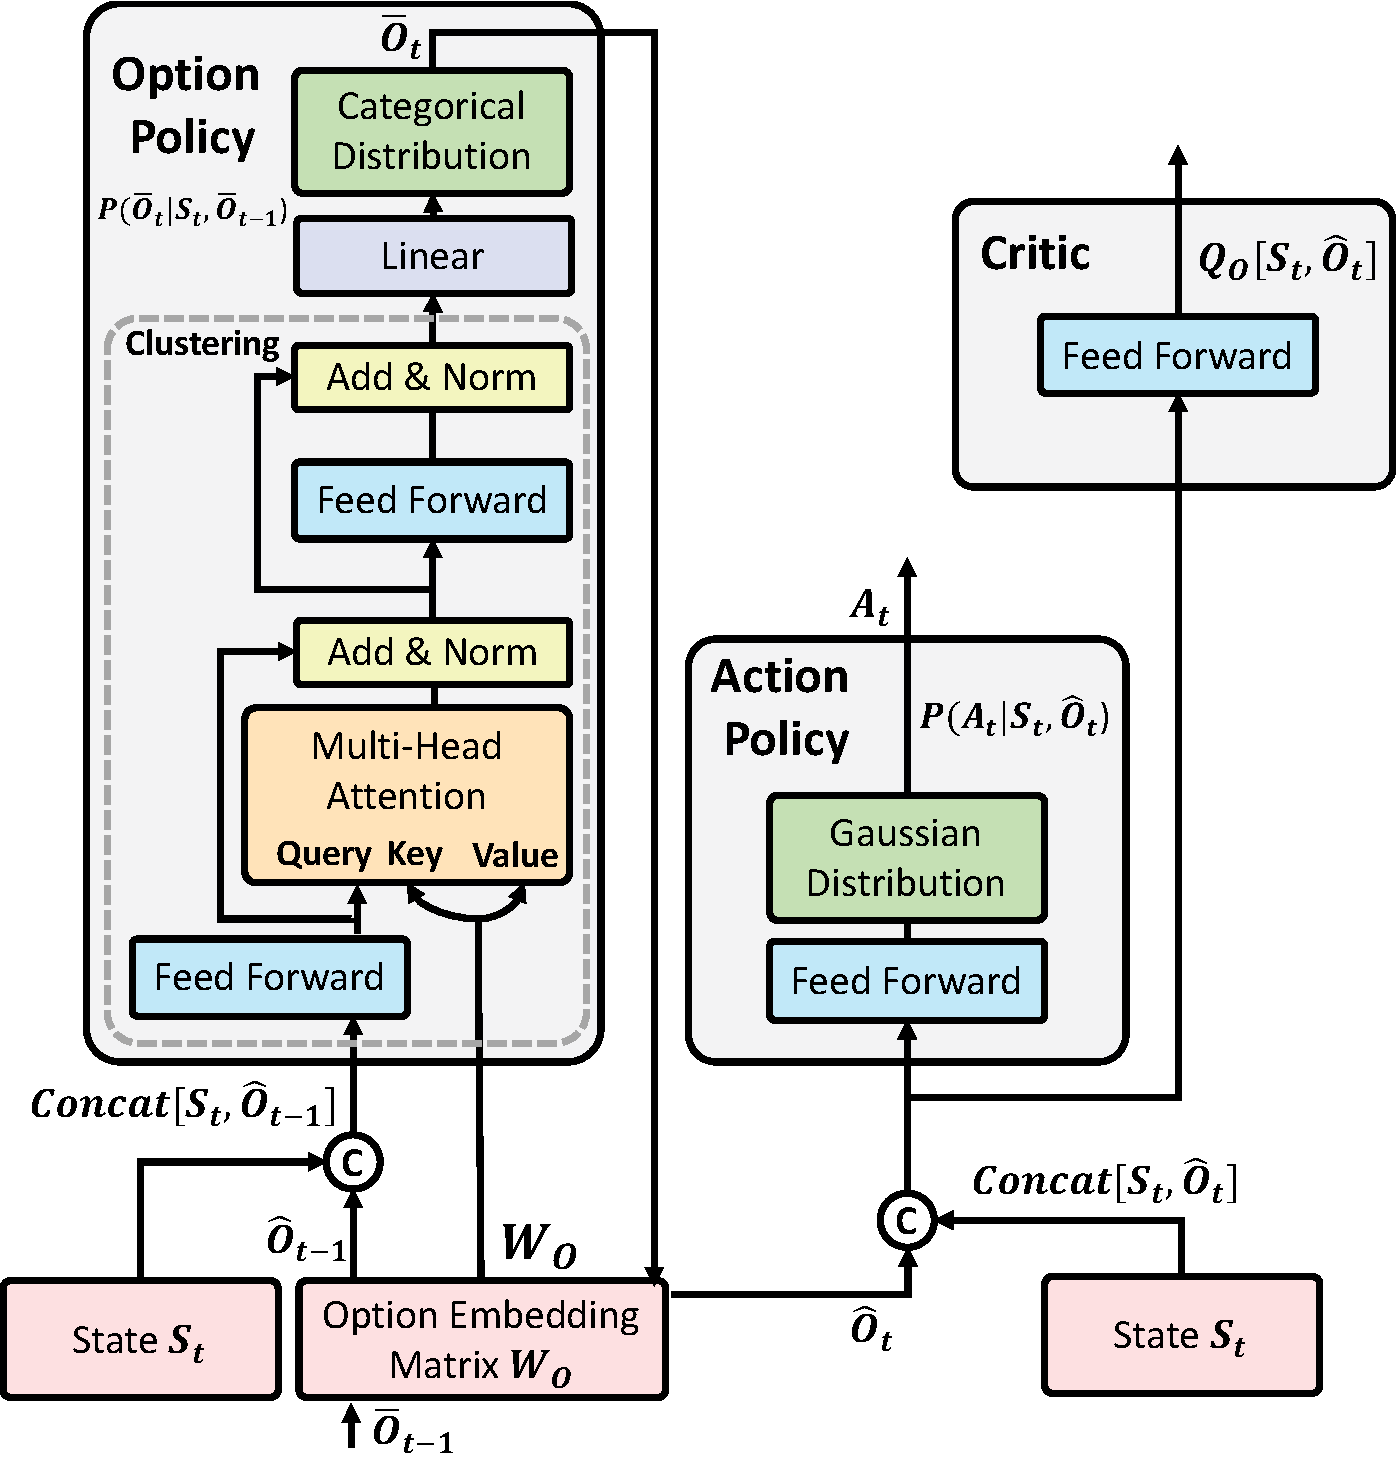
\includegraphics[width=1\linewidth]{./figures/sa_attn_net.png}
  \caption{\label{fig:sa_net} The Option2Vec Architecture}
  \vspace{-5mm}
\end{wrapfigure}

To overcome these difficulties, we significantly improves
\emph{SMDP-Option}'s scalability by redefining options as
distributed representations. In order to achieve this, we first
need to propose a novel option-induced Markov Decision Process
(MDP), the \emph{MDP-Option}. The \emph{MDP-Option} is equivalent
to \emph{SMDP-Option} under the definition of \emph{bisimulation}
\cite{givan2003equivalence}, and compatible with any sample
efficient MDP-style policy optimization algorithms (e.g. PPO
\cite{witoonchart2017application}). The \emph{MDP-Option} enables
simultaneously maintaining the equivalence to \emph{SMDP-Option}
while encoding all local information (where to initiate, what
actions to emit and when to terminate) of an option altogether
into an option embedding $\hat{o}$ (distributed representation).
Option embeddings are essentially clustering centroids on an
Euclidean parametric space \cite{amari1987differential} which is
homeomorphic to the statistical manifold. Because distances
between real vectors (embeddings) are trivial to calculate,
complexities of learning options and classification hyperplanes
are simplified as a clustering problem over option embedding
centroids.

We propose the \emph{Option2Vec} (O2V) architecture, a simple yet
effective Attention \cite{vaswani2017attention} based
Encoder-Decoder architecture to implement such mechanism.
Specifically, an \emph{option policy}
$P(\hat{\rvo}_t|\rvs_t,\hat{\rvo}_{t-1}=\hat{o})$ is employed as
an encoder: given a hyperplane $[\rvs_t,\hat{o}]$, the
\emph{option policy} simply calculates whichever cluster centroid
$\hat{o}^*$ is closest to the hyperplane and assigns it to
$\hat{\rvo}_t=\hat{o}^*$. Since a vector is closest to itself,
the \emph{option policy} has a natural tendency to temporally
extend the option $\hat{o}$ executed from last step. Under this
formulation, option embeddings combine advantages of both
temporal abstraction \cite{sutton1999between} and state
abstraction \cite{knoblock1990learning} on the ambient space of
state space $\sS$ and option space $\sO$. All \emph{option
  embeddings} share a single decoder, the \emph{action policy}
$P(\rva_t|\rvs_t,\hat{\rvo}_t)$, which decodes an embedding
vector $\hat{\rvo}_t$ into concrete actions $\rva_t$. As a
result, adding a new option in O2V is as cheap as adding an
embedding vector, and regardless the number of options are
learned, O2V only needs to approximate two distributions (option
policy and action policy). Empirical studies on challenging
locomotion environments demonstrate that the \emph{MDP-Option}
and O2V exhibit better scalability, smaller variance, faster
convergence and interpretability.



% \begin{figure*}[thb]
%   \centering
%   \begin{tabular}{cc}
%     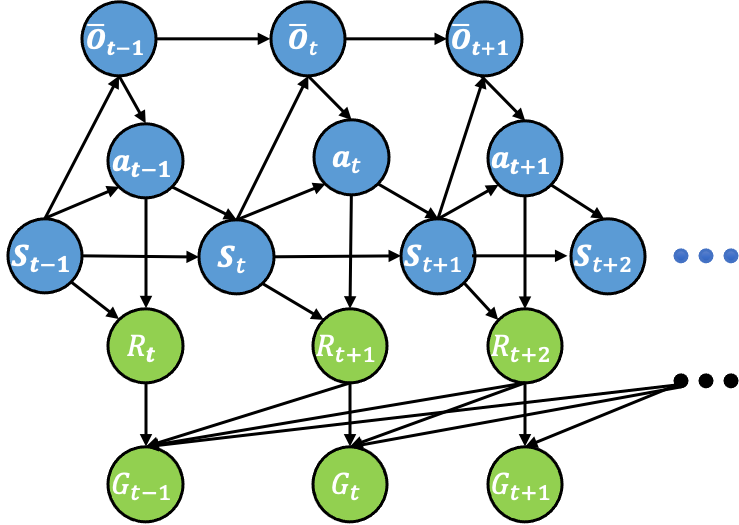
\includegraphics[width=0.45\linewidth]{./figures/doe.png}&
%                                                                \includegraphics[width=0.45\linewidth]{}\\
%     {\small (a) Graphical Model of the MDP-Skill}&
%                                                 {\small (b)  (O2V)}\\
   
%   \end{tabular}\vspace{-2mm}
%   \caption{\label{fig:sa_net} O2V is a Neural Network
%     implementation of the MDP-Skill}
% \end{figure*}


% \begin{figure*}[h]
%   \centering
%   \begin{tabular}{c}
%     
\includegraphics[width=2\columnwidth]{figures/infinite_horizon.png}\\
%     \vspace{-1mm}{\small (a) Infinite Horizon Environments}\\
%     \includegraphics[width=2\columnwidth]{figures/finite_horizon_4.png}\\
%     \vspace{-1mm}{\small (b) Finite Horizon Environments}
%   \end{tabular}\vspace{-2mm}
%   \caption{\label{fig:exp_dac} Episodic Returns. X-axis is time step. Y-axis is
%     Episodic Return}
%   \vspace{-4mm}
% \end{figure*}
With the \emph{MDP-Option} in hand, we can finally move on to
propose the Option2Vec Architecture (O2V). As mentioned in
Section~\ref{sec:sa_PGM}, one major change \emph{MDP-Option} has
been made is that it marginalizes the \emph{mixture master
  policy} and \emph{termination function} away, and models their
marginal distribution, the \emph{skill policy}, directly. In this
section, we demonstrate how O2V temporally extends skills in the
absence of \emph{termination function} by implementing
\emph{MDP-Option} with much more scalable and effective Embedding
and the phenomenal Attention mechanisms
\cite{vaswani2017attention}.

First, one-hot to embedding. one-hot waste, embedding nlp good.
by to embedding, we can: representation good; option is by two
neural nets, scalability 2 nets -> 1 vector. One decoder to
decode all. Decoder can be trained all-time, more sample
efficiency.

1. How options encode temporal abstraction (what is temporal
abstraction), why is this bad?

Integer Index:
integer categories. For example, the identity of option i out of
|O| options can be represented by the

How to describe option's architecture in one term? 1 option 2 nets


2. What is distributed representation? How is skill embedded in
distributed representation?

3. Why embedding good?

gain even more generality and expressivity through a
distributional shift: viewing the identity of an option as
property of the pattern of activation in its vector-valued
representation.

4. How to temporal extension a skill? Why MHA good? MHA >>> termination why?


5. WHy Encoder-Decoder? Save parameters parameter sharing.



% encoder-decoder encode into a compact skill embedding vector

% Interesting extensions to the options framework may be obtained
% by using richer distributions than the categorical case. That is,
% every discrete option is treated as a separate entity
% representing a fixed behavior and its duration. it does a poor
% job at representing knowledge compactly and may require more
% samples than a distributed representations.

% the presence (or absence) of a single bit may not fully signal
% the identity of a chosen option; they would capture different
% aspects of the behavior that the learning system is currently
% trying to produce. Th

% Skill Policy:

% That is, we would need the dis- tribution over next option
% vectors to be more likely to samples similar option vectors as
% the previous ones if the probability of continuing is high. This
% view implies that commitment to an option could be a function not
% only of the termi- nation condition, but also of the width of
% some kernel (a bump) centered on the previous option vector. The
% indicator function of the degenerate component in (3.9) would
% therefore be replaced by a smooth counterpart, where similarity
% would not be established as a hard equality of the form $o_{t+1}=
% o$ but rather as a function of closeness in Euclidean distance to
% the center of that kernel. If the distribution over option
% vectors is binary, it would be more suitable to use a distance
% metric such as the Hamming distance (MacKay, 2002).


% Decoder:

% for example, may correspond to different properties that the
% system ought to see (predict) as a consequence of acting in the
% environment.

% Impact:

% generalization abilities and sample efficiency can be improved.

% would be another mechanism, distinct from parameter sharing, to
% improve generalization.



% % representation good:
% In O2V, knowledge of a skill is explicitly represented as a skill
% context vector (similar to an embedding
% vector~\cite{vaswani2017attention} in Natural Language Processing
% (NLP) or capsule~\cite{sabour2017dynamic} in Computer Vision
% (CV)): each dimension encodes a particular property of the
% skill\footnote{For example, the first dimension may encode the
%   orientation of a primary action. A jump skill context vector
%   may have a large first dimension value which instructs the
%   robot to emit primary actions vertically. A walk skill may have
%   a small value and emit actions horizontally.}. The skill policy
% is similar to a compatibility function: it is used to replace the
% master policy and \emph{termination function} while improving their
% functionalities by employing the attention
% mechanism~\cite{vaswani2017attention}.


% O2V marginalizes the \emph{termination function} away and models
% the marginalization directly with a \emph{skill policy}
% $P(\hat{\rvo}_t|\rvs_t,\hat{\rvo}_{t-1})$. Similar to prove the
% Theorem\ref{theo:smdp_mdp}, we again propose a function
% $\hat{B}(\bar{\rvo})=\bar{\rvo}\cdot W=\hat{\rvo}:
% \{0,1\}^K\rightarrow \sR^{K\times E}$, which maps the one-hot
% index vector $\bar{\rvo}$ to a \emph{skill context vector}
% $\hat{\rvo}_t\in \sR^{E}$, where $\mW_S\in \sR^{K\times E}$ the
% \emph{skill context matrix}, which is a learnable parameter
% containing $K$ rows of $E$ dimensional real vectors, the $i$-th
% row of $\mW_S$ corresponds to the $i$-th skill $\hat{\ro}_i$, and
% different columns encode different properties of a skill. Since
% $\hat{B}$ is a linear function defined on real space, it is also
% a Bijection.




% $P(\bar{\rvo}_t|\rvs_t,\bar{\rvo}_{t-1}=o)$: determining whether
% to terminate the executed option $o$ from last step
% $\bar{\rvo}_{t-1}=o$ is equivalent to examining whether executing
% the option $o$ at time step $t$, namely assigning
% $\bar{\rvo}_t=o$, still has the closest distance to the pair
% $\{\rvs_t,\bar{\rvo}_{t-1}=o\}$. Because a vector is closest to
% itself, the \emph{skill policy} naturally has a tendency to
% continue the option executed from the last step. Since
% calculating distances between $\bar{\rvo}_t$ and
% $\{\rvs_t,\bar{\rvo}_{t-1}=o\}$ is more of architecture
% designations rather than the MDP, 


% It is natural to wonder that how O2V temporally extends an option
% without modeling the \emph{termination function}. In fact, temporal
% relationships between options are explicitly captured in the
% \emph{skill policy} $P(\bar{\rvo}_t|\rvs_t,\bar{\rvo}_{t-1}=o)$:
% determining whether to terminate the executed option $o$ from
% last step $\bar{\rvo}_{t-1}=o$ is equivalent to examining whether
% executing the option $o$ at time step $t$, namely assigning
% $\bar{\rvo}_t=o$, still has the closest distance to the pair
% $\{\rvs_t,\bar{\rvo}_{t-1}=o\}$. Because a vector is closest to
% itself, the \emph{skill policy} naturally has a tendency to
% continue the option executed from the last step. Since
% calculating distances between $\bar{\rvo}_t$ and
% $\{\rvs_t,\bar{\rvo}_{t-1}=o\}$ is more of implementation choices
% rather than the MDP of O2V, we defer this topic to
% Section~\ref{sec:net_arch} and focus this section on proposing
% dynamics of O2V.


% The skill policy which is used to
% replace both the master policy and \emph{termination function} while
% implements their functionalities with the attention
% mechanism~\cite{vaswani2017attention}: since now skills are
% explicitly encoded in embedding vectors $\hat{\rvo}_t$, it is
% trivial to calculate each skill vector's distance to a pair of
% $\{\hat{\rvo}_{t-1},\rvs_t\}$, which contains the skill
% $\hat{\rvo}_{t-1}$ executed from last step together with the
% current state $\rvs_t$. The marginalization over termination
% function can be compensated by the much more powerful Attention
% mechanism, which has been a phenomenal technique in encoding
% long-term dependencies in
% % todo: ViT wrong
% NLP\cite{devlin2018bert} and CV\cite{forney1973viterbi}. With
% MHA, temporal extension of a skill is as simple as selecting
% which $\hat{\rvo}_t$ has the closest distance to the
% $\{\hat{\rvo}_{t-1},\rvs_t\}$ pair. Because one vector is closest
% to itself, O2V naturally has the tendency to continue skill
% executed from the last step. Efficiency of O2V has been witnessed
% in all of our experiments especially infinite-horizon ones.


% After deriving the MDP of O2V, we present a simple neural network
% implementation of the Option2Vec Architecture
% (Figure~\ref{fig:sa_net}). Unlike the conventional SMDP option
% framework, which employs a \emph{termination function} and an SMDP
% master policy to temporally extend the execution of an option, O2V
% implements the temporal extension functionality by employing the
% Multi-Head Attention (MHA) mechanism~\cite{vaswani2017attention}
% (due to page limitations, we briefly explain MHA in
% Appendix~\ref{sec:appen_mha}). At each time step, the skill
% policy $P(\hat{\rvo}_t|\rvs_t,\hat{\rvo}_{t-1};\mW_s)$ attends to
% (measures the compatibility of) all skill context vectors in
% $\mW_s$ according to $\rvs_t$ and $\hat{\rvo}_{t-1}$. If
% $\hat{\rvo}_{t-1}$ still fits $\rvs_t$, then the skill policy
% assigns a larger attention weight to $\hat{\rvo}_{t-1}$, thus has
% a tendency to continue with it. Otherwise, a new skill with
% better compatibility will be sampled. The action policy is as
% simple as one decoder to decode $\hat{\rvo}_t$ and $\rvs_t$ into
% primary actions $\rva_t$. The attention mechanism together with
% skill context vectors enable O2V to temporally extend skills even
% in the absence of \emph{termination function}s.

% Specifically, a \textbf{skill policy} (Eq.~(\ref{eq:sa_o_p}))
% uses a concatenation of current state $\rvs_t$ and previous skill
% context vector $\hat{\rvo}_{t-1}$ as the query for MHA. Both key
% and value matrices are the skill context matrix $\mW_S$. In this
% way, we have:

% \begin{align}
%   \label{eq:sa_net_skill_concat}
%   \hat{\rvs}_{t-1} &= linear(\text{Concat}[\rvs_t,\hat{\rvo}_{t-1}]),\\
%   \label{eq:sa_net_skill_mha}
%   \rvd^O_t &= \text{MHA}(\hat{\rvs}_{t-1},\mW_S,\mW_S),\\
%   \label{eq:sa_net_skill_sample}
%   \rvo_t &\sim Categorical(\rvo_t|\rvd^O_t),
% \end{align}
% where the $linear$ layer simply projects the concatenated vector
% to $E$ dimension. MHA is employed to attend to (measures the
% compatibility of) all skills in $\mW_s$ according to $\rvs_t$ and
% $\hat{\rvo}_{t-1}$. The \textbf{skill density vector} $\rvd^O_t$
% is then used as densities for a Categorical distribution
% $P(\rvo_t|\rvd^O_t)$, from which the new one-hot \textbf{skill
%   index vector} $\rvo_t$ is sampled from. We can retrieve the
% \textbf{skill context vector} by $\hat{\rvo}_t =
% \mW_S^T\cdot\rvo_t$. With the skill context vector $\hat{\rvo}_t$
% in hand, the \textbf{action policy} can be designed as simple as
% a multi-layer Feed-Forward Networks (FFN) decoder:
% \begin{align}
%   \label{eq:sa_net_action_concat}
%   \rvd^A_t &= \text{FFN}(\rvs_t,\hat{\rvo}_{t}),\\
%   \label{eq:sa_net_action_sample}
%   \rva_t &\sim P(\rva_t|\rvd^A_t),
% \end{align}
% where $\rvd^A_t$ is a density vector and $P$ is an arbitrary
% probability distribution (works for both discrete and continuous
% situations).

% Similar to \citename{zhang2019dac}, because of the \textbf{skill
%   value upon arrival function} $V(\rvs_t,\hat{\rvo}_{t-1})$,
% (Eq.~\ref{eq:sa_v}) is an expectation of the \textbf{skill value
%   function} $Q_O[\rvs_{t},\hat{\rvo}_{t}]$ (Eq.~\ref{eq:sa_q_o}).
% It is sufficient for us to model only one critic function:
% \begin{equation}
%   \label{eq:nn_o_input}
%   Q_O=\text{FFN}(\rvs_t,\hat{\rvo}_t),
% \end{equation}
% where $Q_O$ is implemented as a multi-layer FFN. We summarize the
% detailed learning procedures in Algorithm~\ref{alg:sa} in
% Appendix~\ref{sec:append_algo}.

% Since $\hat{\rvo}_t$ encodes all context of a skill, O2V only
% needs one action policy decoder to decode the activated skill
% context vectors $\hat{\rvo}_t$ and current state $\rvs_t$ into
% primary actions $\rva_t$. This design choice largely improves the
% scalability of O2V: adding one more skill is as cheap as adding a
% skill context vector. Moreover, unlike the option framework, in
% which only the activated option's action policy gets updated, the
% action policy learns to decode each dimension of skill context
% vectors at every time step. This design choice largely improves
% sample efficiency and enables O2V to converge faster than the
% conventional option framework.

% % % todo: layer by layer training
% % % todo: training layer by layer proof
% % \vspace{-3mm}
% % \section{Experiments}
% % \label{sec:exp}
% % \vspace{-2mm}

% % \begin{figure*}[h]
% %   \centering
% %   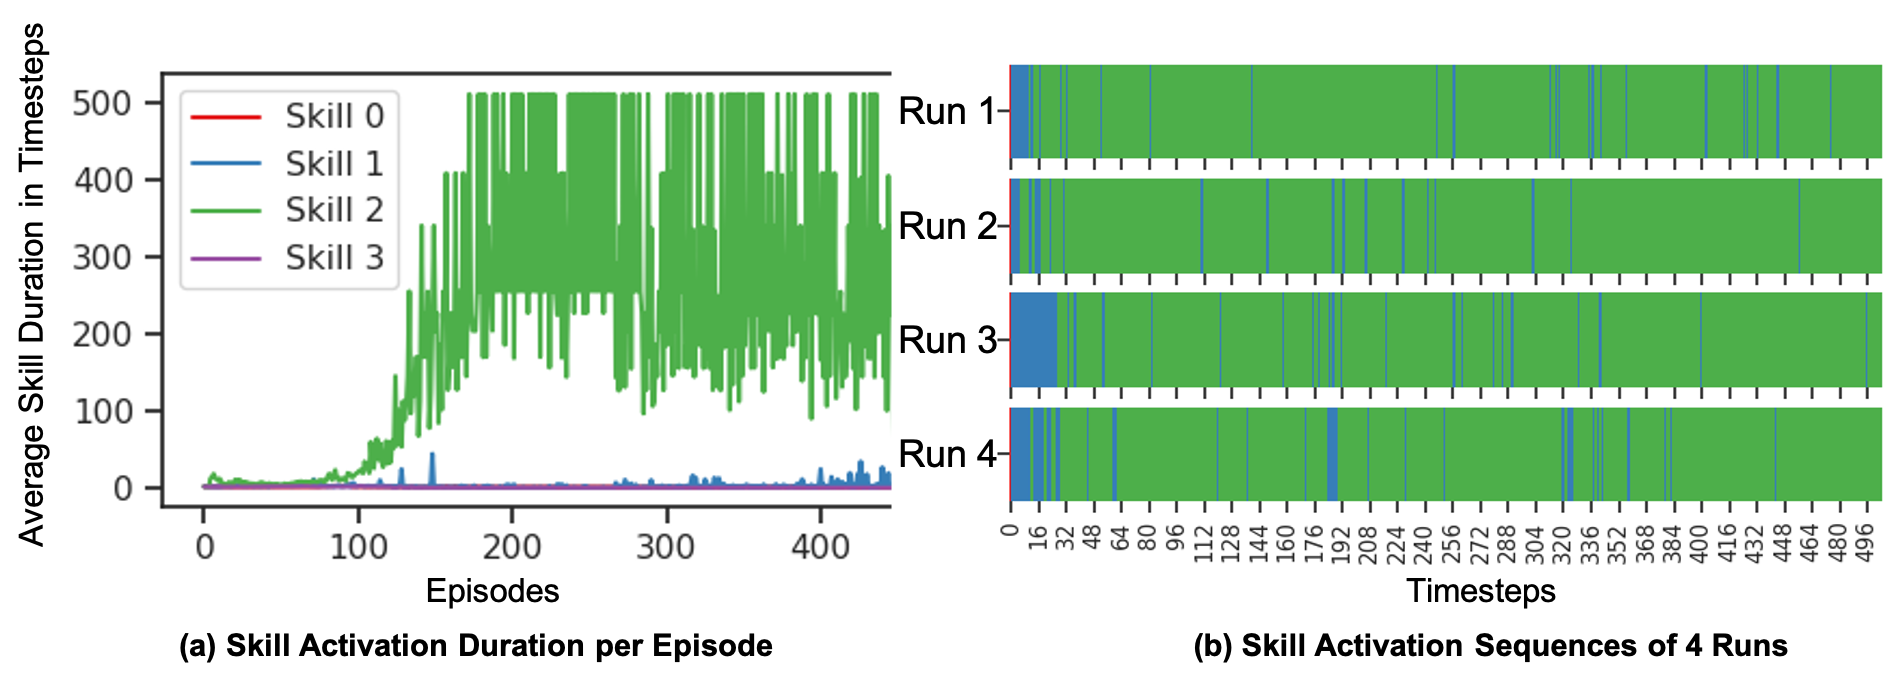
\includegraphics[width=0.7\linewidth]{./figures/skill_sequence_joint.png}\\
% %   \vspace{-4mm}\caption{\label{fig:skill_sequence} Skill Duration
% %   Patterns}\vspace{-3mm}
% % \end{figure*}
% % \begin{figure*}[h]
% %   \centering
% %   \includegraphics[width=0.75\linewidth]{./figures/Interp_joint.png}\\
% %   \vspace{-4mm}\caption{\label{fig:interp_joint} Interpretation
% %     of Skill Context Vectors}\vspace{-4mm}
% % \end{figure*}

% % % to write: in this section,
% % In this section, we design experiments to answer three questions:
% % 1) Can O2V outperform other baselines (regarding episodic returns,
% % stability, and scalability)? 2) Can O2V temporally extend skills
% % without the \emph{termination function}? 3) Can skill context vectors be
% % easily interpreted? 4) Does skill embeddings learned by O2V have a
% % performance boost over other option variants in transfer learning
% % settings?

% % For single task learning, experiments are conducted on all OpenAI
% % Gym MuJoCo environments (10 environments)
% % \cite{brockman2016openai}. We follow DAC~\cite{zhang2019dac} and
% % compare our algorithm with five baselines, four of which are
% % option implementations, i.e., DAC+PPO \cite{zhang2019dac},
% % AHP+PPO \cite{levy2011unified}, IOPG \cite{smith2018inference}, PPOC
% % \cite{klissarov2017learnings} and OC \cite{bacon2017option}. The
% % last baseline is PPO \cite{schulman2017proximal}. All baselines'
% % parameters used in DAC\footnote{All baselines' implementations
% %   are from DAC's open source repo
% %   https://github.com/ShangtongZhang/DeepRL/tree/DAC. Note that
% %   the author list of this paper does not have any overlap with
% %   DAC. Our source code is available in supplementary materials.}
% % remain unchanged other than the maximum number of training steps:
% % O2V only needs 1 million steps to converge rather than the 2
% % million used in DAC. For transfer learning, we follow
% % \citename{zhang2019dac} and run 6 pairs of transfer learning
% % tasks constructed in DAC based on DeepMind Control Suite
% % \cite{tassa2020dmcontrol}. For a fair comparison, we use four
% % skills for O2V and four options for other option implementations.
% % All experiments are run on an Intel® Core™ i9-9900X CPU @ 3.50GHz
% % with a single thread and process. Our implementation details are
% % summarized in Appendix~\ref{sec:append_implement}.

% % \begin{figure*}[h]
% %   \vspace{-2mm}
% %   \centering
% %   \includegraphics[width=1\linewidth]{./figures/transfer.png}\\
% %   \vspace{-4mm}
% %   \caption{\label{fig:transfer} Performance on DAC transfer
% %     learning tasks}
% %   \vspace{-4mm}
% % \end{figure*}

% % \subsection{Single Task Learning}
% % \label{sec:exp_perf}
% % \vspace{-2mm}
% % % towrite: figure capitalize
% % In Figure~\ref{fig:exp_dac}, we report episodic returns on
% % infinite horizon and finite horizon\footnote{We refer to
% %   environments with the game-over condition as finite horizon
% %   environments, and infinite vice versa.} environments
% % separately. For a fair comparison, we use exactly the same
% % plotting script as used in DAC: curves are averaged over 10
% % independent runs and smoothed by a sliding window of size 20.
% % Shaded regions indicate standard deviations. Performance of all
% % ten environments is shown in (Appendix
% % Figure~\ref{fig:all_tasks}, Table~\ref{table:single_infinite}).

% % It is extremely interesting that O2V shows two completely
% % different kinds of behaviors on infinite and finite horizon
% % environments. According to previous option framework
% % implementations~\cite{klissarov2017learnings,smith2018inference,harb2018waiting,zhang2019dac},
% % on single task environments, option-based algorithms do not have
% a distinguishable performance boost over hierarchy-free
% algorithms. O2V also has similar behavior and achieves comparable
% performance to the best baseline algorithm on most finite horizon
% environments (Figure~\ref{fig:exp_dac} (b)). In
% Appendix~\ref{sec:append_gist} we conceptually explain that
% conventional value functions are insufficient to approximate
% models which have temporal latent variables dependencies. A
% concrete deep wide skill-action architecture remains open for the
% future work.

% On infinite horizon environments as shown in
% Figure~\ref{fig:exp_dac} (a), O2V's performance significantly
% outperforms all baselines by a large margin in various aspects.
% For episodic return, e.g., HumanoidStandup, all option
% implementations barely converge, while O2V is $240\%$ better than
% DAC and AHP\footnote{Even on Reacher, a simple environment on
%   which most algorithms converge to a similar performance, O2V is
%   still $38\%$ better than the second best (AHP).}. For
% convergence, O2V has the fastest convergence speed. On the first
% two environments, which are also reported in DAC, O2V only takes
% $40\%$ of time steps of DAC and AHP to reach similar episodic
% returns. This acceleration is because: 1) O2V is MDP formulated,
% the skill policy is updated at each time step; 2) O2V only has one
% action policy decoder; 3) the action decoder learns to decode
% skill context vectors whichever skill is activated. For
% stability, all 10 runs of O2V converge to a similar level while
% the other have much larger standard deviations. This property is
% theoretically justified by Proposition~\ref{prop:var_red} and
% further discussed in Appendix~\ref{sec:append_gist}.

% \vspace{-2mm}
% \subsection{Temporal Extension}
% \label{sec:exp_ext}

% It is logical to ask whether O2V is capable of temporal extension
% without the \emph{termination function}. To illustrate this, we plot the
% average duration of each skill during training episodes of the
% HalfCheetah environment in Figure~\ref{fig:skill_sequence} (a)
% and 4 runs of skill activation sequences in
% Figure~\ref{fig:skill_sequence} (b). (more details in
% Appendix~\ref{sec:append_exp_ext}). At the start of training, all
% skills' durations are short, while Skill 2's duration quickly
% grows and dominates the entire episode. This growth of duration
% proves that O2V can still temporally extend a skill. Towards the
% end of the training, the dominant skill's duration starts to
% decrease while the duration of a secondary skill (Skill 1) starts
% to increase. This means that during later training stages, O2V
% starts to coordinate different skills. The dominant skill
% phenomenon is also reported in other option implementations such
% as DAC. However, as shown in the
% video\footnote{https://www.youtube.com/watch?v=QiLVZvI6NJU}, O2V
% still learns distinguishable skills. Skill 2 is the running
% forward skill thus it dominates the whole episode. Skill 1 is
% only used to recover from falling down thus it has much shorter
% duration. As discussed in Appendix \ref{sec:append_gist},
% solution to the dominant skill is actually learning skills at
% much finer granularity. The O2V-style wide value function
% (Eq.~(\ref{eq:sa_v})) provides an elegant solution to this
% problem.

% \vspace{-2mm}
% \subsection{Interpretation of Skill Context Vectors}
% \label{sec:interpret}

% Explicit skill representations not only improve efficiency,
% scalability, and generalization, but also benefit interpretation.
% We continue with the HalfCheetah example and demonstrate how
% easily skill context matrix $\mW_s$
% (Figure~\ref{fig:interp_joint} (a)) can be interpreted (more
% details are provided in Appendix~\ref{sec:append_interpret}). We
% first follow \citename{sabour2017dynamic} and interpret what
% property is represented by a context vector's dimension by adding
% perturbations on to it, and inspecting perturbations' effects
% on the action policy decoder in generating primary actions $\rva$
% (Figure~\ref{fig:interp_joint} (b)). Once each dimension is
% understood, skills become straight forward to interpret by simply
% inspecting on which dimensions (property) each skill $\hat{\rvo}$
% in Figure ~\ref{fig:interp_joint} (a) has significant weights,
% and interpreting properties of those dimensions
% ((Figure~\ref{fig:interp_joint} (c)). In this way, we can
% interpret that Skill 2 is a forward movement skill, since it
% focuses on jumping and running forward, while Skill 1 is a
% landing skill. These interpretations can further be used to
% explain skill activation patterns in
% Figure~\ref{fig:skill_sequence} (b): Skill 2 has the longest
% duration because it is the major source of all forward movements.
% Skill 2 occasionally falls back to Skill 1 because, after jumping
% or running, the HalfCheetah needs to land and balance itself.


% \subsection{Transfer Learning}
% \label{sec:transfer}

% We follow \citename{zhang2019dac} and run 6 pairs of transfer
% learning tasks constructed in DAC based on DeepMind Control Suite
% \cite{tassa2020dmcontrol}. Each pair contains two different
% tasks. To keep consistent with DAC, we train all models one
% million steps on the first task and switch to the second (O2V's
% skill context matrix is subsequently frozen) to run another one
% million steps. Results are reported in Figure~\ref{fig:transfer}
% (Appendix Table~\ref{table:transfer}). On the first task, O2V's
% performance is among the best algorithms in all environments.
% This further validates O2V's advantages on single task as observed
% in section~\ref{sec:exp_perf}. On the transfer learning (the
% second) task, O2V's performance ranks the first in 5 out of 6
% environments. This shows O2V's advantages in knowledge reuse
% tasks. \vspace{-2mm}


\section{Related Works}
\label{sec:review}

As a result, most option variants compromise to only two-level
SMDP because the number of options grows exponentially with
levels \cite{riemer2018learning}; the initiation set is widely
ignored because of difficulties in learning it from data
\cite{khetarpal2020options}. Moreover, learning switching
between options is analogously learning classification
hyperplanes on the statistical manifold, in a linear case, for
$N$ hyperplanes, theoretically there are $2^N$ options to be
learned with \cite{mankowitz2016adaptive}.

% % % todo: SMDP-style MDP-style
% % To discover options automatically, \citename{sutton1999between}
% % proposed Intra-option Q-learning to update the master Q value
% % function at every time step. However, all policies under this
% % formulation are approximated implicitly using the Q-learning
% % method. \citename{levy2011unified} proposed to unify the
% % Semi-Markov process into an augmented Markov process and
% % explicitly learn an ``overall policy'' by applying MDP-based
% % policy gradient algorithms. However, their method for updating
% % the master policy is still SMDP-style thus sample inefficient.
% % \citename{bacon2017option} proposed a policy gradient based
% % Option Critic (OC) framework for explicitly learning intra-option
% % policies and \emph{termination function}s in an intra-option manner.
% % However, for the master policy's policy gradients learning, OC
% % still remains SMDP-style. \citename{klissarov2017learnings}
% % attempted to combine OC with PPO in an intra-option learning
% % manner (PPOC). However, as we show in
% % Appendix~\ref{sec:appen_hmm}, due to the SMDP formulation,
% % gradients they use for updating master policy are inconsistent.
% % \citename{zhang2019dac} reformulated the option framework into
% % two augmented MDPs. Under this formulation all policies can be
% % modeled explicitly and learned in MDP-style. However, their model
% % is still expensive to scale up. On single task environments, DAC
% % has no significant advantages over other baselines.

We must appreciate that \citename{bacon2018temporal} (Chapter 3.5
and 3.6) first conceptually discussed the possibility of
introducing the skill policy and distributed representations into
the option framework. However, to the best of our knowledge, this
is the first concrete work that discovers and proves the MDP
equivalence of the SMDP-Option, and enables learning options as
distributed representations. Although sharing similar
formulations with \cite{bacon2018temporal}, our work is motivated
by causal reinforcement learning
\cite{peters2016causal,doshi2016hidden} and capsule networks
\cite{sabour2017dynamic} (more details in
Appendix~\ref{sec:append_gist}) and is developed independently
from \cite{bacon2018temporal}.

% % With respect to optimization, \citename{zhang2019dac} pointed out
% % that a large margin of performance boost of DAC comes from
% % Proximal Policy Optimization \cite{schulman2017proximal} (PPO).
% % Since O2V is MDP-based, it can be optimized directly with the PPO.
% % Recent works show that the option framework trained under
% % off-policy \cite{haarnoja2018soft} algorithms outperforms
% % on-policy methods. For instance, HO2 \cite{wulfmeier2020data}
% % employs a trust-region constrained off-policy algorithm and shows
% % that it exhibits significant advantages over on-policy methods on
% % both sample efficiency and performance. In this paper, we propose
% % O2V as a general HRL framework which can be trained by both
% % on-policy and off-policy algorithms. Our main contribution
% % focuses on deriving MDPs of O2V and its policy gradient theorems.
% % Designing off-policy algorithms for O2V remains open for future
% % work.

% % Existing RL literature
% % \cite{hausman2018learning,li2017infogail,tirumala2019exploiting}
% % also uses latent variables to learn skill embeddings. Typically,
% % PEARL \cite{rakelly2019efficient} learns a latent context vector
% % for each task under the meta-reinforcement learning framework to
% % improve the agent's sample and transfer learning efficiency.
% % However, embeddings learned by RL frameworks only encode action
% % level abstraction while O2V learns abstractions at both action and
% % temporal levels. It is also worth to mention that, the novel
% % formulation of O2V establishes a strong connection to causal
% % reinforcement learning. When the number of skills equals one
% % ($M=1$), O2V falls back to Generalized Hidden Parameter MDPs
% % (GHP-MDPs) \cite{kolobov2012discovering,perez2020generalized}.
% % Causality properties of O2V is a direction worth to be explored in
% % the future work.

% % % parameter vector in policy to encode causality between policy and
% % % environment properties. Causality properties of O2V is a direction
% % % worth to be explored in the future work. There are also
% % % interesting attempts to introduce supervised guidance into HRL
% % % \cite{gupta2019relay}. With hierarchical knowledge explicitly
% % % represented in embedding matrix, O2V provides a more efficient and
% % % scalable HRL model for such frameworks.

\section{Conclusions}
\label{sec:conclusion}
\vspace{-2mm}

In this paper, we presented a novel MDP equivalence of the SMDP
formulated option framework, from which an MDP implementation of
the option framework, i.e., the Option2Vec architecture, was
derived. We theoretically proved that O2V has lower variance than
conventional RL models and provided policy gradient theorems for
updating O2V. Our empirical studies on challenging infinite
horizon robot simulation environments demonstrated that O2V not
only outperforms all baselines by a large margin, but also
exhibits smaller variance, faster convergence, and good
interpretability. On transfer learning, O2V also outperforms the
other models in 5 out of 6 environments and shows its advantages
in knowledge reuse tasks.

The final and most important contribution of O2V is hierarchically
learning explicit abstract actions' representations with ``skill
context vectors''. This design significantly improves the
scalability and interpretability of O2V. It is straightforward to
extend O2V to deeper and wider (Appendix~\ref{sec:append_gist})
architectures, which gives rise to a large-scale pre-training and
transfer learning architecture in the reinforcement learning
area.


% % \subsubsection*{Acknowledgments}
% % We thank Shangtong Zhang for his great open source project. We
% % deeply appreciate Pierre-Luc Bacon, Matthew D Riemer and
% % Shangtong Zhang's patience in answering our questions.

\bibliography{Bibs/hrl,Bibs/fin,Bibs/lit,Bibs/sa,Bibs/causal,Bibs/IL}
\bibliographystyle{icml2021}




% \begin{ack}
% Use unnumbered first level headings for the acknowledgments. All acknowledgments
% go at the end of the paper before the list of references. Moreover, you are required to declare
% funding (financial activities supporting the submitted work) and competing interests (related financial activities outside the submitted work).
% More information about this disclosure can be found at: \url{https://neurips.cc/Conferences/2021/PaperInformation/FundingDisclosure}.

% Do {\bf not} include this section in the anonymized submission, only in the final paper. You can use the \texttt{ack} environment provided in the style file to autmoatically hide this section in the anonymized submission.
% \end{ack}

% \section*{References}

% References follow the acknowledgments. Use unnumbered first-level heading for
% the references. Any choice of citation style is acceptable as long as you are
% consistent. It is permissible to reduce the font size to \verb+small+ (9 point)
% when listing the references.
% Note that the Reference section does not count towards the page limit.
% \medskip

% {
% \small

% [1] Alexander, J.A.\ \& Mozer, M.C.\ (1995) Template-based algorithms for
% connectionist rule extraction. In G.\ Tesauro, D.S.\ Touretzky and T.K.\ Leen
% (eds.), {\it Advances in Neural Information Processing Systems 7},
% pp.\ 609--616. Cambridge, MA: MIT Press.

% [2] Bower, J.M.\ \& Beeman, D.\ (1995) {\it The Book of GENESIS: Exploring
%   Realistic Neural Models with the GEneral NEural SImulation System.}  New York:
% TELOS/Springer--Verlag.

% [3] Hasselmo, M.E., Schnell, E.\ \& Barkai, E.\ (1995) Dynamics of learning and
% recall at excitatory recurrent synapses and cholinergic modulation in rat
% hippocampal region CA3. {\it Journal of Neuroscience} {\bf 15}(7):5249-5262.
% }

% %%%%%%%%%%%%%%%%%%%%%%%%%%%%%%%%%%%%%%%%%%%%%%%%%%%%%%%%%%%%
% \section*{Checklist}

% %%% BEGIN INSTRUCTIONS %%%
% The checklist follows the references.  Please
% read the checklist guidelines carefully for information on how to answer these
% questions.  For each question, change the default \answerTODO{} to \answerYes{},
% \answerNo{}, or \answerNA{}.  You are strongly encouraged to include a {\bf
% justification to your answer}, either by referencing the appropriate section of
% your paper or providing a brief inline description.  For example:
% \begin{itemize}
%   \item Did you include the license to the code and datasets? \answerYes{See Section~\ref{gen_inst}.}
%   \item Did you include the license to the code and datasets? \answerNo{The code and the data are proprietary.}
%   \item Did you include the license to the code and datasets? \answerNA{}
% \end{itemize}
% Please do not modify the questions and only use the provided macros for your
% answers.  Note that the Checklist section does not count towards the page
% % limit.  In your paper, please delete this instructions block and only keep the
% % Checklist section heading above along with the questions/answers below.
% % %%% END INSTRUCTIONS %%%

% % \begin{enumerate}

% % \item For all authors...
% % \begin{enumerate}
% %   \item Do the main claims made in the abstract and introduction accurately reflect the paper's contributions and scope?
% %     \answerTODO{}
% %   \item Did you describe the limitations of your work?
% %     \answerTODO{}
% %   \item Did you discuss any potential negative societal impacts of your work?
% %     \answerTODO{}
% %   \item Have you read the ethics review guidelines and ensured that your paper conforms to them?
% %     \answerTODO{}
% % \end{enumerate}

% % \item If you are including theoretical results...
% % \begin{enumerate}
% %   \item Did you state the full set of assumptions of all theoretical results?
% %     \answerTODO{}
% % 	\item Did you include complete proofs of all theoretical results?
% %     \answerTODO{}
% % \end{enumerate}

% % \item If you ran experiments...
% % \begin{enumerate}
% %   \item Did you include the code, data, and instructions needed to reproduce the main experimental results (either in the supplemental material or as a URL)?
% %     \answerTODO{}
% %   \item Did you specify all the training details (e.g., data splits, hyperparameters, how they were chosen)?
% %     \answerTODO{}
% % 	\item Did you report error bars (e.g., with respect to the random seed after running experiments multiple times)?
% %     \answerTODO{}
% % 	\item Did you include the total amount of compute and the type of resources used (e.g., type of GPUs, internal cluster, or cloud provider)?
% %     \answerTODO{}
% % \end{enumerate}

% % \item If you are using existing assets (e.g., code, data, models) or curating/releasing new assets...
% % \begin{enumerate}
% %   \item If your work uses existing assets, did you cite the creators?
% %     \answerTODO{}
% %   \item Did you mention the license of the assets?
% %     \answerTODO{}
% %   \item Did you include any new assets either in the supplemental material or as a URL?
% %     \answerTODO{}
% %   \item Did you discuss whether and how consent was obtained from people whose data you're using/curating?
% %     \answerTODO{}
% %   \item Did you discuss whether the data you are using/curating contains personally identifiable information or offensive content?
% %     \answerTODO{}
% % \end{enumerate}

% % \item If you used crowdsourcing or conducted research with human subjects...
% % \begin{enumerate}
% %   \item Did you include the full text of instructions given to participants and screenshots, if applicable?
% %     \answerTODO{}
% %   \item Did you describe any potential participant risks, with links to Institutional Review Board (IRB) approvals, if applicable?
% %     \answerTODO{}
% %   \item Did you include the estimated hourly wage paid to participants and the total amount spent on participant compensation?
% %     \answerTODO{}
% % \end{enumerate}

% % \end{enumerate}

% % %%%%%%%%%%%%%%%%%%%%%%%%%%%%%%%%%%%%%%%%%%%%%%%%%%%%%%%%%%%%

% % \appendix

% % \section{Appendix: Learning Skills at Multi-levels of Granularity}
% % \label{sec:append_gist}

% % Implementations of the option framework share some common
% % limitations. When proposing the option framework,
% % \citename{sutton1999between} expected that learning at
% % multi-level of temporal abstraction should be in favor of faster
% % convergence and better exploration. On the contrary, significant
% % improvements on single task environments have not been witnessed
% % in most option
% % implementations~\cite{klissarov2017learnings,smith2018inference,harb2018waiting,zhang2019dac}.
% % To the best of our knowledge, O2V is the first option
% % implementation in which these properties are significantly
% % witnessed but only on infinite horizon environments. In this
% % section, we address this problem by first giving a theoretical
% % explanation of why the value function is the main reason for this
% % deficiency in section~\ref{sec:append_turkey} and how
% % \textbf{deep wide value functions} could solve this problem. We
% % then thoroughly explain the motivations of O2V, and why it is a
% % promising candidate for a deep wide framework, in
% % section~\ref{sec:append_dwsa}. We also give a further explanation
% % of how O2V is connected to causality reinforcement learning
% % literature and how a temporal causal reward can be used in
% % objective to further solve this problem in
% % section~\ref{sec:append_causal_rew}.

% % \subsection{Problem Statement and Evidences}
% % \label{sec:append_turkey}

% % The expectation of improvements of the option framework on single
% % task environment builds on an assumption that, by exploiting
% % hierarchical action and state space, an agent's searching space
% % can be greatly reduced thus accelerates learning and improving
% % exploration. However, as reported in section~\ref{sec:exp_ext},
% % most option frameworks including O2V suffer from ``the dominant
% % skill problem'' \cite{zhang2019dac} which prevents option
% % frameworks from effectively learning hierarchy in action and
% % state space as well as coordinating between skills.

% % One root reason for this problem is that conventional value
% % functions $V[S_t]$ and $Q[S_t,O_t,A_t]$ make values depend on
% % temporal latent variables indistinguishable (i.e. Although
% % different skills $o_1$ and $o_2$ results to different values,
% % such as $V[S_t,O_{t-1}=o_1]=10$ and $V[S_t,O_{t-1}=o_2]=-10$.
% % Because they arrive at the same state $S_t$, they have identical
% % values under conventional value function $V[S_t]=0$). This
% % deficiency makes option frameworks can only learn skills at very
% % coarse level thus fail to exploit hierarchical information. The
% % solution is to use a \textbf{deep wide value function}: enabling
% % the framework to learn fine-grained skills at mutli-levels of
% % granularity (deep) and making value functions depend on latent
% % variables with longer (wide) dependencies (e.g. $V[S_t,O_{t-1}]$
% % and $Q[S_t,O_t,A_t,O_{t-1}]$).

% % To have a better understanding the importance of the deep wide
% % value function, let us consider a simple environment which can be
% % easily solved by $Q[s_t,a_t,a_{t-1}]$ but not $Q[s_t,a_t]$.

% % Suppose we are training a robot which only has a camera sensor to
% % cook thanksgiving turkey. In this setting there are only two
% % states: $\sS=\{\text{Raw Turkey Image},\text{Cooked Turkey
% %   Image}\}$. The robot's action space only consists of two
% % actions: $\sA=\{\text{Stuff turkey},\text{Roast turkey}\}$. As
% % for reward, if the robot roasted a stuffed turkey, then the
% % reward is $10$. However, if the robot roasted an un-stuffed
% % turkey, then the reward is $-10$. The $\text{stuff turkey}$
% % action receives $0$ reward.

% % The difficulty in this environment is, since the robot only has a
% % camera to capture an image of the turkey, it can only observes
% % either $\{\text{Raw Turkey Image}\}$ or $\{\text{Cooked Turkey
% %   Image}\}$. There is no way to look inside the turkey and see if
% % the turkey is stuffed. Under this setting, a robot can never
% % learn to first stuff a turkey and then roast it because
% % $Q[\text{Raw Turkey Image},\text{Stuff Turkey}] = Q[\text{Raw
% %   Turkey Image},\text{Roast Turkey}] = 0$. Therefore, the robot
% % can only randomly cook a turkey. However, this problem can be
% % easily solved by using a deep wide value function
% % $Q[S_t,A_t,A_{t-1}]$.

% % The core problem in this setting is, action has no effect on
% % states, it only affects rewards. At the first glance this is a
% % Partially Observed MDP (POMDP) problem since the state of whether
% % the turkey is stuffed is un-observed. This is true in all
% % reinforcement learning settings without dependencies on latent
% % variables. However, it goes much deeper in HRL settings.

% % In HRL, a common formulation is to estimate a latent variable $O$
% % to encode hierarchical information and makes the policy depends
% % on it $P(A_t|S_t,O_t)$. Since $O$ is a latent variable, it is
% % highly likely that at state $S_t$, different latent variable
% % $P(A_t|S_t,O_t=o_x)$ and $P(A_t|S_t,O_t=o_y)$ emits the same
% % action $A_t=A_1$, and thus makes the conventional value function
% % indistinguishable between $o_x$ and $o_y$.

% % This phenomenon is especially common around the switching time
% % step of two skills: around switching point, states are usually
% % compatible with both old and new skills. Conventional value
% % functions will be especially confused at those moments. This is
% % exactly what we observed in Figure~\ref{fig:skill_sequence}:
% % overall, skill 2 is executed consistently. However, there are
% % some random switches to skill 1. And the randomization is
% % increased between around switching time steps. To explicitly show
% % this, we visualized ``Run4'' into a video:
% % $\text{https://www.youtube.com/watch?v=QiLVZvI6NJU}$. The skill
% % selection is very random at the beginning of the episode as well
% % as around the switching point (the 16th second). These are
% % exactly the most confusing moments of conventional value
% % functions. This is not a cherry-pick result but a common problem.
% % Similar patterns can also be observed here
% % $\text{https://youtu.be/xrfxbI3duBM?t=4}$ in a HumanoidStandUp
% % environment.

% % Due to the insufficiency of conventional value functions,
% % compatible states have to be different enough to cause
% % distinguishable values of value functions. Therefore, with
% % conventional value functions, O2V is only able to learn very
% % coarse skills. For example, as shown in
% % Figure~\ref{fig:interp_joint} and the video, the HalfCheetah
% % agent is only able learn two skills: one is to run forward, one
% % is to stand up when fall. However it is not able to learn more
% % fine-grained skills such as jump forward and landing. This
% % problem is not limited to O2V, but is a common problem in HRL. The
% % solution is to use deep wide value functions.

% % \subsection{Motivations behind O2V's Architecture}
% % \label{sec:append_dwsa}

% % O2V is carefully designed to make the most out of deep wide value
% % functions. Compared to other HRL frameworks, O2V has following
% % advantages: 

% % \begin{enumerate}
% % \item Stable and unbiased estimation: Thanks to
% %   proposition~\ref{prop:var_unb} and \ref{prop:var_red}, the
% %   higher the order of the MDPs, the smaller the variance will be.
% %   The deep wide value functions stays unbiased estimations of
% %   conventional value functions no matter how many dependencies
% %   introduced. The current solution in option framework is a
% %   biased estimation \cite{harb2018waiting} and adding
% %   hyper-parameters to the framework.
% % \item Easy to incorporate wide value functions: Incorporating a
% %   deep wide value function is straightforward, O2V's \textbf{skill
% %     value upon arrival function} is already a wide function. The
% %   \textbf{skill value function} and the \textbf{skill-action
% %     value function} can be easily extended to wide function by
% %   adding a first-order dependency on $\hat{O}_{t-1}$.
% % \item Easy to incorporate deep value functions: O2V is MDP
% %   formulated, extending O2V to multiple hierarchies is
% %   straightforward.
% % \item Scalability to long time dependencies: O2V is MDP
% %   formulated, adding more time dependencies is simply to change
% %   the 1st-order MDP to higher-order MDPs while both value
% %   functions and gradient theorems stay unchanged; O2V is attention
% %   based, O2V can easily attends to thousand time steps without
% %   adding any extra complexity to neither skill policy nor action
% %   policy.
% % \item Scalability to multiple hierarchies of skills: O2V is
% %   attention based and embedding based. Adding skills is as simple
% %   as adding skill context matrix. In traditional option
% %   frameworks \cite{riemer2018learning}, the number of option
% %   (note that each option is a neural network) grows at $O(N^L)$
% %   complexity of levels ($N$ is the number of options and $L$ is
% %   the number of levels).
% % \item Interpretability. As shown in section~\ref{sec:interpret},
% %   skill context vectors learned under O2V-based architectures are
% %   straightforward to visualize and interpret. This property is
% %   especially useful for investigating multi-level granularity
% %   skills.
% % \end{enumerate}

% % \subsection{Causality Discovery Rewards}
% % \label{sec:append_causal_rew}

% % Although theoretically a DWO2V can learn multi-level granularity
% % skills, on-policy optimization algorithm is often insufficient
% % for learning such models especially in sparse reward
% % environments. However, O2V has a natural connection with causal
% % reinforcement learning thus can exploits causality as a reward in
% % objective function to further facilitate fine grained skill
% % discovery. In this section we explain how skill embedding vectors
% % learned by O2V encodes temporal causality relationships and how to
% % use them to devise causal rewards.

% % In causal reinforcement learning area, \citename{doshi2016hidden}
% % proposed Hidden Parameters MDP (Hi-MDP) in which a skill vector
% % like hidden parameter vector is introduced to learn abstract
% % properties from environments. PEARL \cite{rakelly2019efficient}
% % utilizes meta-learning framework to learn a skill representation
% % that encodes abstract properties of a task and updates the
% % framework in an off-policy manner to improve sample efficiency in
% % transfer learning. \citename{killian2017robust} extended Hi-MDP
% % by including the hidden parameter vector into transition
% % probability function. \citename{perez2020generalized} further
% % extended their work by proposing Generalized Hidden Parameter
% % MDPs (GHP-MDPs), a causality discovery framework by including
% % hidden parameter vector into both transition function and value
% % function.

% % GHP-MDPs is a special case of O2V with number of skills $M=1$.
% % When $M>1$, O2V not only encodes causality relationships between
% % environments and actions but also temporal causality between
% % skills. Since the latent variable is modeled as a skill vector,
% % the distance between different trajectories is straightforward to
% % be calculated and thus can be used as a causal reward to
% % encourage fine-grained and disentangled skills' discovery. To the
% % best of our knowledge, O2V is the first RL framework concerns
% % causality in temporal abstraction sequences. We focus this paper
% % on proposing O2V, the causality rewarded O2V will be discussed in
% % future works.

% % Another interesting understanding of O2V is that, rather than an
% % implementation of the option framework, O2V can also be seen as a
% % novel capsule network~\citename{kosiorek2019stacked} trained by
% % policy gradient theorems. In Stacked Capsule Auto-Encoders (SCAE)
% % \cite{kosiorek2019stacked}, a ``capsule'' vector encodes a
% % different property (scale, orientation, etc.) of the visual
% % object in each dimension. \citename{kosiorek2019stacked} proposed
% % to delegate the complexity of part objects detection and
% % part-to-whole objects aggregation by employing the attention
% % mechanism \cite{lee2019set} on which a generative model is then
% % built to further decode the whole-part relationships. This design
% % choice abstracts the complexity of inference away from the
% % decoder and largely simplified the designation of the generative
% % model.

% % In this paper, we follow their motivations of learning better
% % representations and utilizing the attention mechanism to simplify
% % the inference problem (sampling new skill without termination
% % function). Moreover, the skill context vector is analogously to a
% % capsule and the skill-action relationship is analogously to the
% % whole-part relationship in the SCAE. Similar to SCAE utilizing
% % the equi-variance property of the whole-part relationship to
% % achieve computing efficiency and better performance, it will be
% % very exciting to investigate potentially ``equi-variance'' or
% % ``invariance'' properties existed in skill-action relationships,
% % which might give rise to a novel causal inference architecture in
% % the reinforcement learning area.

% % \section{Experiments Results}
% % \label{sec:append_exp}
% % \subsection{Performance}
% % \label{sec:append_exp_perf}

% % In this section we provide results for all ten OpenAI Gym Mujoco
% % Environments. Those environments can be classified into two categories:
% % infinite horizon environments (i.e., HalfCheetah, Swimmer,
% % HumanoidStandup and Reacher) and finite horizon environments (the
% % other).
% % \begin{figure*}[thb]
% %   \centering
% %   \includegraphics[width=1\linewidth]{./figures/all_exps.png}\\
% %   \caption{\label{fig:all_tasks} Performance of Ten OpenAI Gym
% %     MuJoCo Environments.}
% % \end{figure*}

% % \begin{table*}[]
% % \caption{Performance of Infinite Horizon Environments}
% % \label{table:single_infinite}
% % \vskip 0.15in
% % \begin{center}
% % \begin{tabular}{|l|l|l|l|l|}
% % \hline
% %         & HalfCheetah        & Swimmer           & HumanoidStandup     & Reacher          \\ \hline
% % PPO     & 2143.6                & 59.9                 & 62262.2                & -7.5                \\ \hline
% % DAC+PPO & 1830.1                & 85.0                 & 38954.9                & -8.1                \\ \hline
% % AHP+PPO & 1701.7                & 86.7                 & 38684.9                & -7.3                \\ \hline
% % PPOC    & 1441.2                & 43.6                 & 39841.7                & -9.4                \\ \hline
% % OC      & 832.3                 & 33.0                 & 52352.7                & -15.3               \\ \hline
% % O2V+PPO  & {\ul \textbf{3446.7}} & {\ul \textbf{107.8}} & {\ul \textbf{91654.5}} & {\ul \textbf{-4.6}} \\ \hline
% % \end{tabular}
% % \end{center}
% % \vskip -0.1in
% % \end{table*}

% % \begin{table*}[]
% % \caption{Performance of Finite Horizon Environments}
% % \label{table:single_finite}
% % \vskip 0.15in
% % \begin{center}
% % \begin{tabular}{|l|l|l|l|l|l|l|}
% % \hline
% %         & Walker2d           & Hopper             & InvertedPendulum  & InvertedDoublePendulum & Ant                & Humanoid          \\ \hline
% % PPO     & 1512.5                & 1489.9                & 939.9                & 7112.6                    & 1049.6                & 562.1                \\ \hline
% % DAC+PPO & {\ul \textbf{1968.0}} & 1702.2                & {\ul \textbf{943.7}} & 5804.5                    & 985.8                 & 487.6                \\ \hline
% % AHP+PPO & 1520.6                & {\ul \textbf{1993.6}} & 940.0                & {\ul \textbf{7120.7}}     & {\ul \textbf{1359.3}} & {\ul \textbf{569.3}} \\ \hline
% % PPOC    & 756.1                 & 1308.1                & 936.2                & 7117.6                    & 429.4                 & 483.9                \\ \hline
% % OC      & 391.9                 & 487.6                 & 207.1                & 2369.4                    & 433.4                 & 475.1                \\ \hline
% % O2V+PPO  & 1856.9                & 1955.3                & 906.5                & 6884.1                    & 907.4                 & 528.7                \\ \hline
% % \end{tabular}
% % \end{center}
% % \vskip -0.1in
% % \end{table*}

% % \newpage
% % \subsection{Temporal Extension}
% % \label{sec:append_exp_ext}

% % In Figure~\ref{fig:duration}, we plot the average duration of
% % each skill during 430 training episodes (each episode contains a
% % trajectory of 512 time steps) of the HalfCheetah environment. In this
% % environment, the agent learns to run half of a Cheetah by controlling 6
% % joints: back thigh, back shin, back foot, front thigh, front
% % shin, and front foot. The faster the Cheetah runs forward, the
% % higher return it gets from the environment. At the start of
% % training, all skills' durations are short. After the $100$-th
% % episode, Skill 2's duration quickly grows and dominates the
% % entire episode. The dominant skill phenomenon is also reported in
% % other option implementations such as DAC. One explanation for
% % this domination phenomenon is that for some single task environments,
% % primitive actions might be enough to express the optimal policy,
% % in which case extra levels of abstraction (skills) become
% % overhead. However, because the duration of dominant skill starts
% % to fall at the end of training and O2V significantly outperforms
% % PPO which only employs primary actions, these facts indicate that
% % O2V has a better capability of automatically discovering abstract
% % actions from primary actions as well as coordinating between
% % them.
% % \begin{figure*}[thb]
% %   \centering
% %   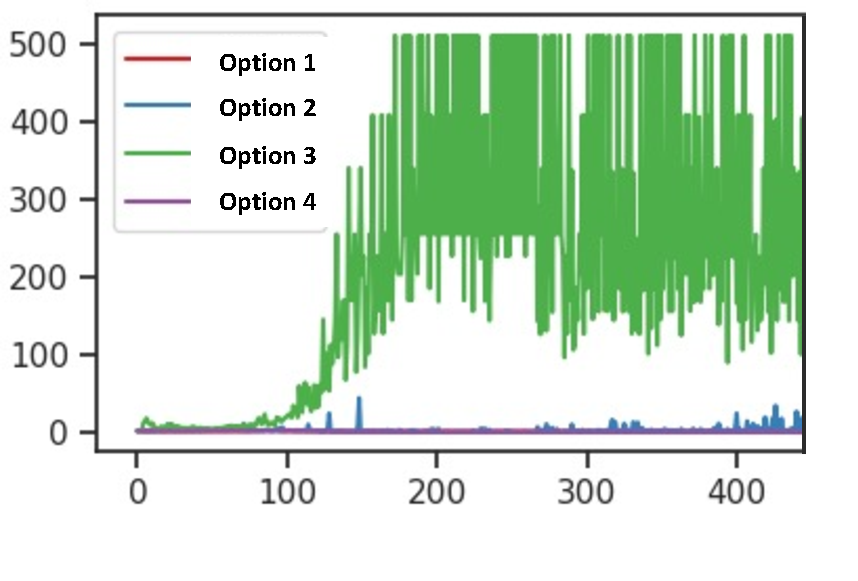
\includegraphics[width=0.7\linewidth]{./figures/duration.png}\\
% %   \caption{\label{fig:duration} Duration of 4 options during 430
% %     training episodes of HalfCheetah.}
% % \end{figure*}

% % To illustrate how O2V coordinates
% % skills, we take the HalfCheetah model trained after 1 million
% % steps and independently run it 4 times (4 episodes. each episode
% % contains 512 time steps). Skill activation sequences of 4 runs
% % are then plotted in Figure~\ref{fig:option_pattern}.
% % \begin{figure*}[thb]
% %   \centering
% %   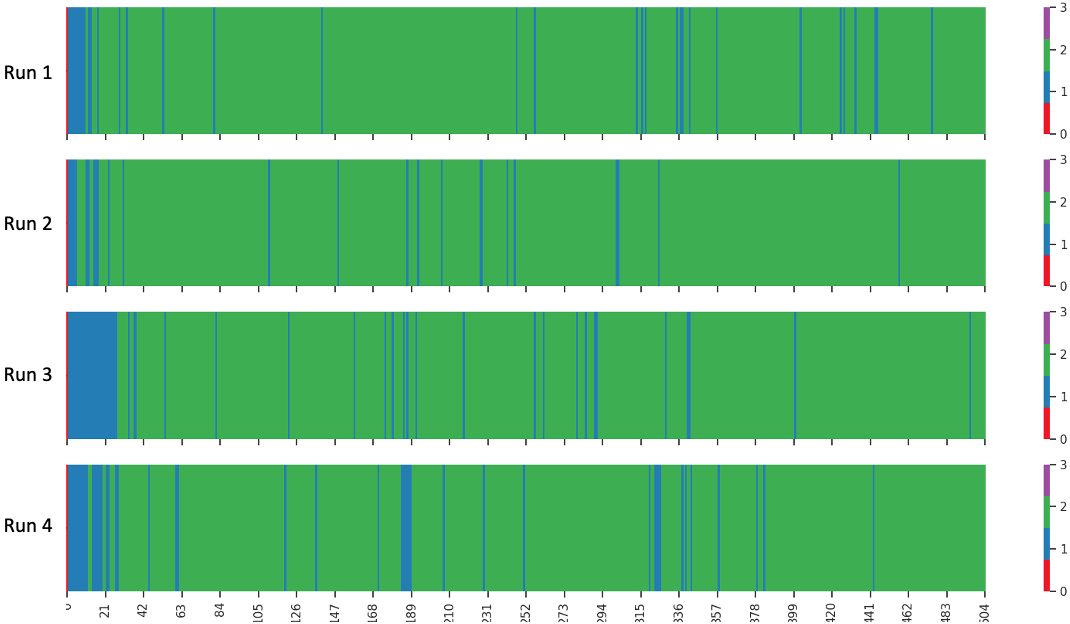
\includegraphics[width=0.7\linewidth]{./figures/option_pattern.png}\\
% %   \caption{\label{fig:option_pattern} Activated option sequences
% %     of 4 independent HalfCheetah runs.}
% % \end{figure*}
% % As we can see that there are some common patterns between all 4
% % independent runs. For example, all runs start with Skill 0 and
% % use Skill 1 at the early stage. After executing Skill 1 for a
% % short period, they all switch to Skill 2 which has longest
% % durations in all 4 runs. From time to time they will fall back to
% % Skill 1 for short periods and quickly switch to Skill 2 again.
% % This pattern of coordination indicates that Skill 1 and Skill 2
% % have completely different functionality and O2V has the capability
% % of automatically discovering as well as leveraging those
% % skills.

% % \subsection{Interpretation of Skill Context Vectors}
% % \label{sec:append_interpret}

% % In this section we continue with the HalfCheetah model used in
% % Section~\ref{sec:append_exp_ext} and demonstrate how to interpret
% % skill context vectors as well as skill activation sequences
% % (Figure \ref{fig:option_pattern}). In HalfCheetah, the agent
% % learns to run half of a Cheetah by controlling 6 joints: back
% % thigh, back shin, back foot, front thigh, front shin, and front
% % foot. The faster the Cheetah runs forward, the higher return it
% % gets from the environment. We interpret skill context vectors and
% % activation patterns by first inspecting what property each
% % dimension of the skill context vector encodes (Figure
% % \ref{fig:first_dim_perturb}). Once each dimension is understood,
% % skills (Figure \ref{fig:all_skill_vectors}) become straight
% % forward to interpret by simply inspecting on which dimension
% % (property) they have the most significant weights (Figure
% % \ref{fig:interp_skill}). These interpretations can further be
% % taken to explain skill activation patterns in Figure
% % \ref{fig:option_pattern}.
% % \begin{figure*}[thb]
% %   \centering
% %   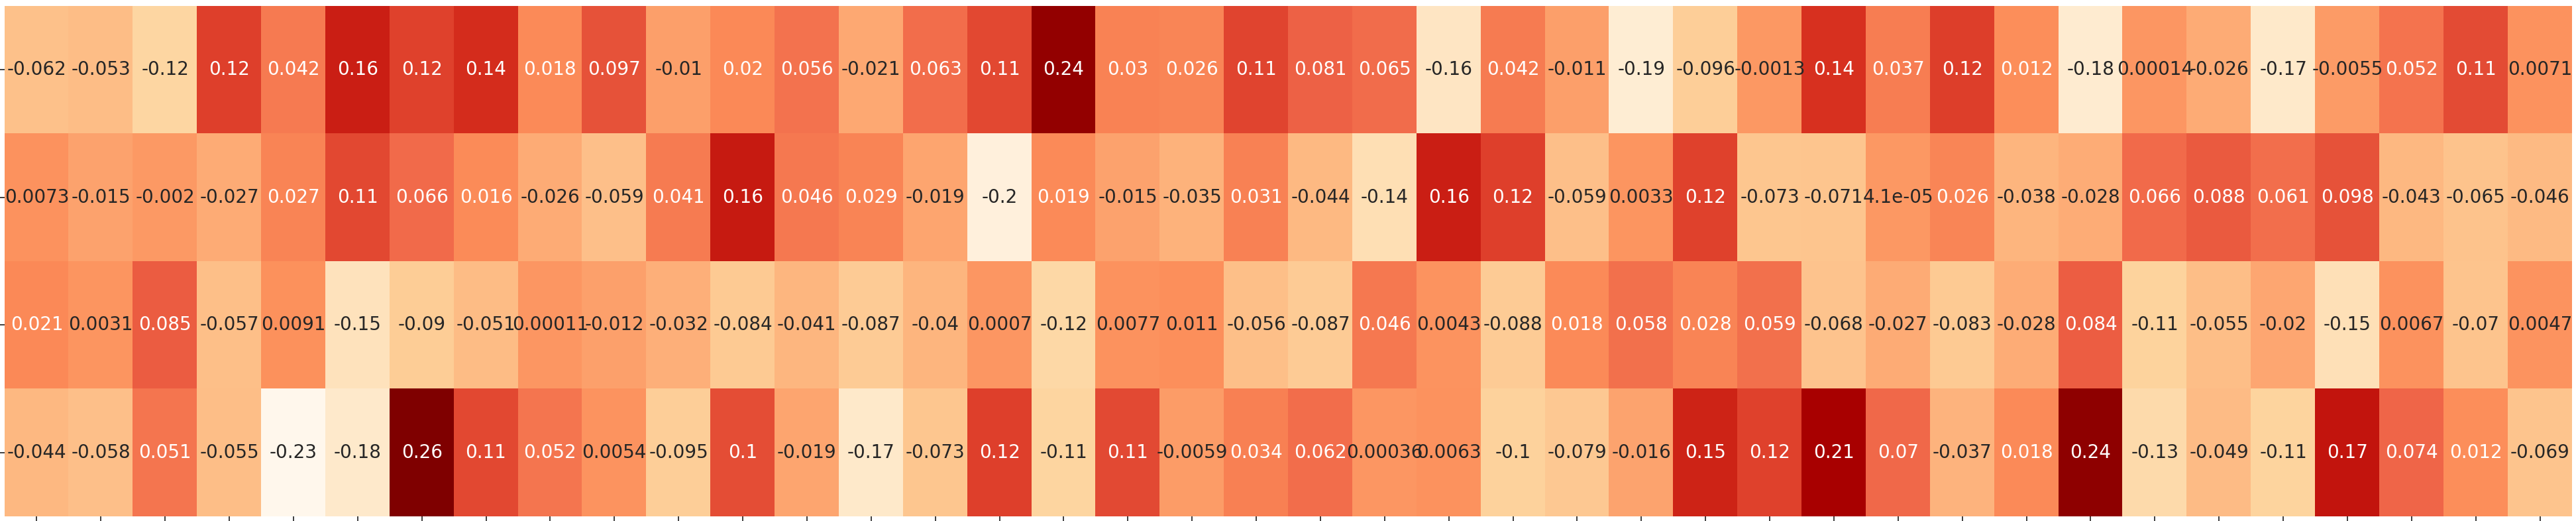
\includegraphics[width=1\linewidth]{./figures/all_skill_vectors.png}\\
% %   \caption{\label{fig:all_skill_vectors} Heatmap of all 4 skill
% %     context vectors}
% % \end{figure*}

% % As the first step, we follow \citename{sabour2017dynamic} to
% % interpret what property each dimension of the skill context
% % vector in Figure~\ref{fig:all_skill_vectors} encodes by
% % perturbing each dimension and decode perturbed skill context
% % vectors into primary actions. Specifically, we perturb one
% % dimension by adding a range of perturbations $[{-0.1}, 0.09]$ by
% % intervals of $0.01$ onto it while keep the other dimensions
% % fixed. After perturbation, each skill context vector dimension
% % has $20$ perturbed vectors. We then use the action policy decoder
% % to decode all those vectors into primary actions and see how the
% % perturbation affects the primary action. As an illustration, we
% % plot Dimension 0's all $20$ perturbed results in Figure
% % \ref{fig:first_dim_perturb}.
% % \begin{figure*}[thb]
% %   \centering
% %   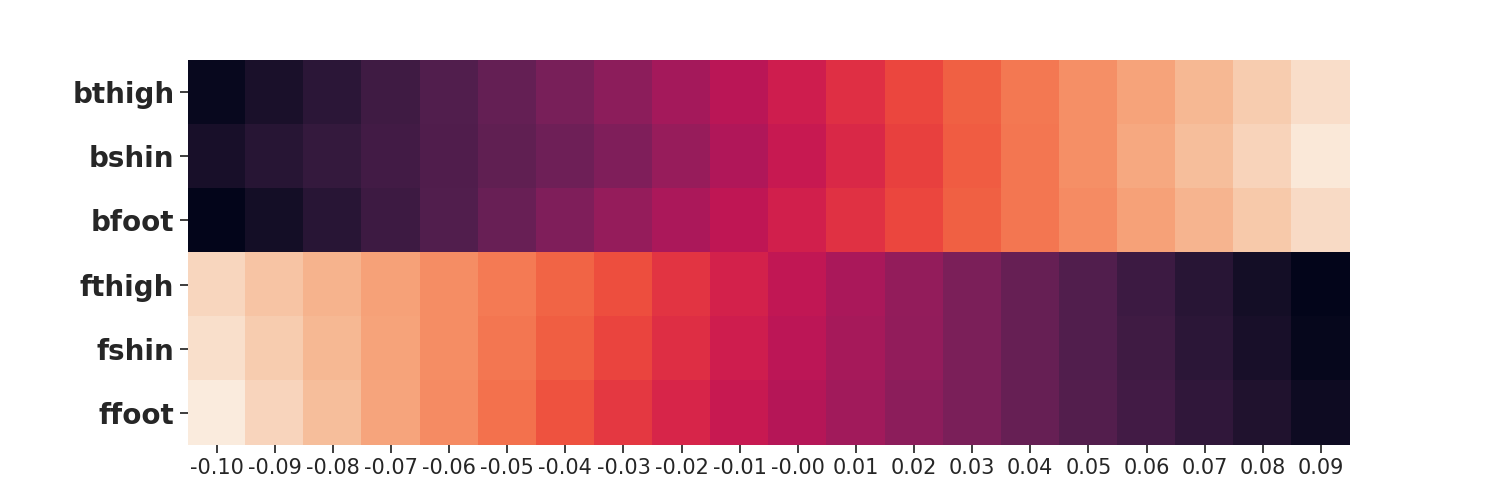
\includegraphics[width=1\linewidth]{./figures/skill_heatmap.png}\\
% %   \caption{\label{fig:first_dim_perturb} Perturbation on the
% %     Dim 0}
% % \end{figure*}

% % With visualization of perturbation results in hand, we can
% % interpret what property each dimension encode by inspecting
% % relationships between perturbations and primary actions. In
% % Figure \ref{fig:first_dim_perturb}, as an example, it is clear
% % that changes on Dim $0$ has opposite effect on the back leg and
% % front leg: a larger value on Dim $0$ will assign the back leg a
% % larger torque while the front leg a smaller one, and vice versa.
% % This means Dim $0$ is has a focus point property: it focuses
% % torque on only one leg.

% % Once we know how to interpret one dimension, we can move on to
% % interpret the whole skill context vector. Since Skill $1$ and
% % Skill $2$ are two main skills employed in
% % Figure~\ref{fig:option_pattern}, here we provide an example of
% % how to interpret them. Figure~\ref{fig:all_skill_vectors} shows
% % that Skill $1$ has significant values on dimension $11$, $15$ and
% % $22$. Skill $2$ is significant on dimension $2$, $5$ and $36$. We
% % demonstrate these dimensions in the same manner as
% % Figure~\ref{fig:first_dim_perturb} below:
% % \begin{figure*}[thb]
% %   \centering
% %   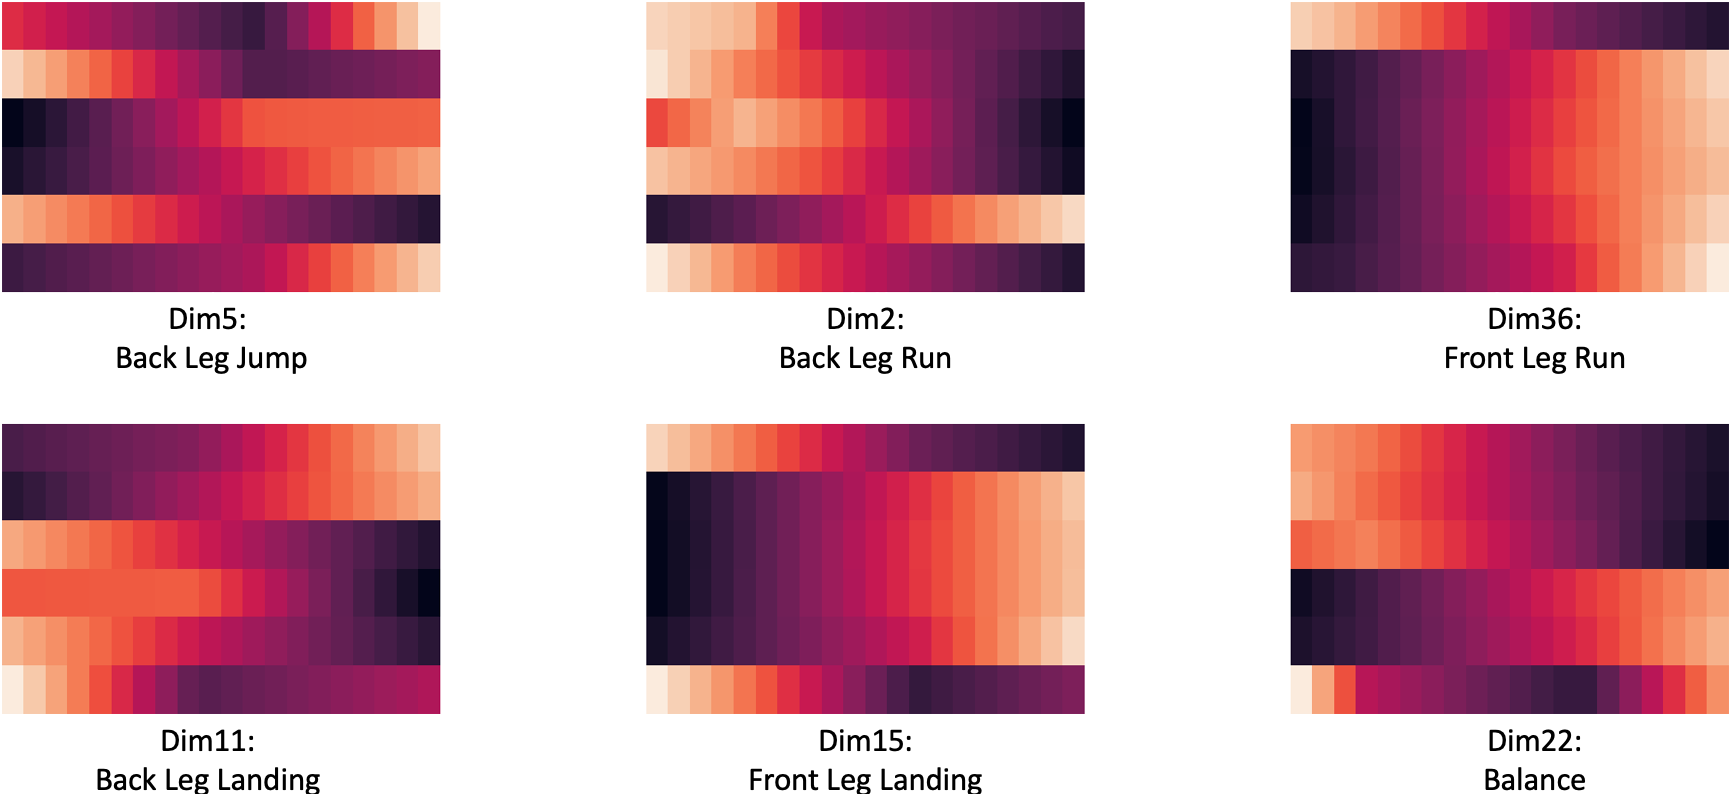
\includegraphics[width=1\linewidth]{./figures/interp_2_skills.png}\\
% %   \caption{\label{fig:interp_skill} Interpretation of Skill 1
% %     and Skill 2}
% % \end{figure*}

% % Subfigures in Figure~\ref{fig:interp_skill} can be interpreted in
% % the same manner as Figure~\ref{fig:first_dim_perturb}. As an
% % example, from Figure~\ref{fig:all_skill_vectors} we can see that
% % Skill $1$ has a significant small value on Dim $11$. In
% % Figure~\ref{fig:interp_skill}, it shows that a smaller Dim $11$
% % will twist the front leg forward and back foot forward while
% % twist back thigh, back shin backward. Composition of these
% % movements is a back leg landing property. Similarly, we can
% % interpret that Dim $15$ is a front leg landing property and Dim
% % $22$ is a balancing property. Therefore, Skill $1$ is focusing on
% % landing from all positions.

% % Unlike other skill context vectors which have apparent focusing
% % dimensions, Skill $2$ has a rather balanced skill context vector.
% % It has no apparently dominant dimension. It only has slightly
% % more significant values on Dim $2$, $5$, $36$, which are focusing
% % on jumping and running properties. Therefore, Skill $2$ is more
% % like an ``all-weather'' skill: it is a skill having very balanced
% % properties with a slightly demonstration on running and jumping.

% % Interpretations of Skill $1$ and $2$ above can then be taken to
% % understand skill activation patterns in
% % Figure~\ref{fig:option_pattern}: as an all-weather skill, Skill
% % $2$ is the most frequently executed one and has the longest
% % duration. From time to time, when the Cheetah needs to land and
% % balance itself, Skill $1$ will be executed. However, since
% % landing skill does not provide power of moving forward and thus
% % has lower returns to continue, once the body is balanced the
% % Cheetah will quickly stop Skill $1$'s execution and keep running
% % with Skill $2$.

% % \subsection{Transfer Learning Results}
% % \label{sec:append_transfer}

% % \begin{table*}[h]
% % \caption{Performance of Deepmind Control Suite Transfer Learning Environments}
% % \label{table:transfer}
% % \begin{center}
% % \begin{tabular}{|l|l|l|l|l|l|l|}
% % \hline
% %         & CartPole             & Reacher              & Cheetah              & Fish                 & Walker1              & Walker2              \\ \hline
% % PPO     & 829.7                & 327.6                & 73.0                 & 287.9                & 231.8                & 72.2                 \\ \hline
% % DAC+PPO & 970.8                & 517.2                & 211.2                & 505.4                & {\ul \textbf{590.3}} & 360.5                \\ \hline
% % AHP+PPO & 966.5                & 395.2                & 167.4                & 357.9                & 362.1                & 143.2                \\ \hline
% % PPOC    & 942.1                & 400.1                & 72.7                 & 336.7                & 236.6                & 80.9                 \\ \hline
% % OC      & 106.1                & 19.4                 & 100.6                & 286.6                & 356.3                & 238.7                \\ \hline
% % O2V+PPO  & {\ul \textbf{974.1}} & {\ul \textbf{675.3}} & {\ul \textbf{233.8}} & {\ul \textbf{562.1}} & 473.8                & {\ul \textbf{403.0}} \\ \hline
% % \end{tabular}
% % \end{center}
% % \end{table*}


% \section{MDP Equivalence to the SMDP Option Framework}
% \label{sec:appen_oc_pgm}

% In this section, we show that the the conventional Semi-Markov
% Decision Problem (SMDP) option framework which employs Markovian
% options actually has an MDP equivalence. We first follow
% \citename{bishop2006pattern}'s method and formulate the dynamics
% of the option framework as an Hidden Markov Model
% (HMM)~\cite{bishop2006pattern} in section~\ref{sec:appen_hmm}.
% With Probability Graphical Model (PGM)~\cite{bishop2006pattern}
% and its conditional independence relationships (Chapter 8.2.1
% \cite{bishop2006pattern}) in hand, we then move on to prove that
% MDP formulation has identical value functions
% (section~\ref{sec:appen_mdp}), bellman equations as well as
% intra-option policy and termination policy gradients to SMDP
% formulation (section~\ref{sec:appen_mdp_grad}). To the best of
% our knowledge, this is the first work discovering the option
% framework's MDP equivalence and deriving the option framework
% from a PGM view.

% \subsection{Background: The Option Framework}
% \label{sec:appen_oc_background}

% \citename{sutton1999between} proposed the option framework to
% demonstrate the temporal abstraction problem. A scalar
% $\ro\in\sZ$ denotes the index of an option where $\sO \subseteq
% \{1,2,\ldots,M\}$ and $M$ is the number of options. An Markovian
% option is a triple $(\sI_{o},P_{o}(\rva|\rvs),P_{o}(\rb|\rvs))$
% % $(\sI_{o_t},P_{o_t}(\rva_t,|\rvs_t),P_{o_t}(\rb_t|\rvs_t))$
% in which $\sI_{o}\subseteq\sS$ is an initiation set where the
% option $o$ can be initiated. $P_{o}(\rva|\rvs):\sS\rightarrow\sA$
% is the intra-option policy which maps environment states
% $\rvs\in\sS$ to an action vector $\rva\in \sA$.
% $P_{o}(\rb|\rvs):\sS\rightarrow\sZ_2$ is a \emph{termination function}
% where $\rb$ is a binary random variable. It is used to determine
% whether to terminate ($\rb=1$) the policy $P_{o}(\rva|\rvs)$ or
% not ($\rb=0$). Conventionally, $\beta_o=P_o(\rb=1|\rvs)$. Since
% an option's execution may persist over a variable period of time,
% a set of options' execution together with its value functions
% constitutes a Semi-Markov Decision Problem (SMDP)
% \cite{puterman2014markov}. When an old option is terminated, a
% new option will be sampled from the master policy
% (policy-over-options) $o\sim P(o_{t+1}|\rvs_{t+1}):
% \sS\rightarrow\sO$.
% \begin{figure*}[th!]
%   \centering
%   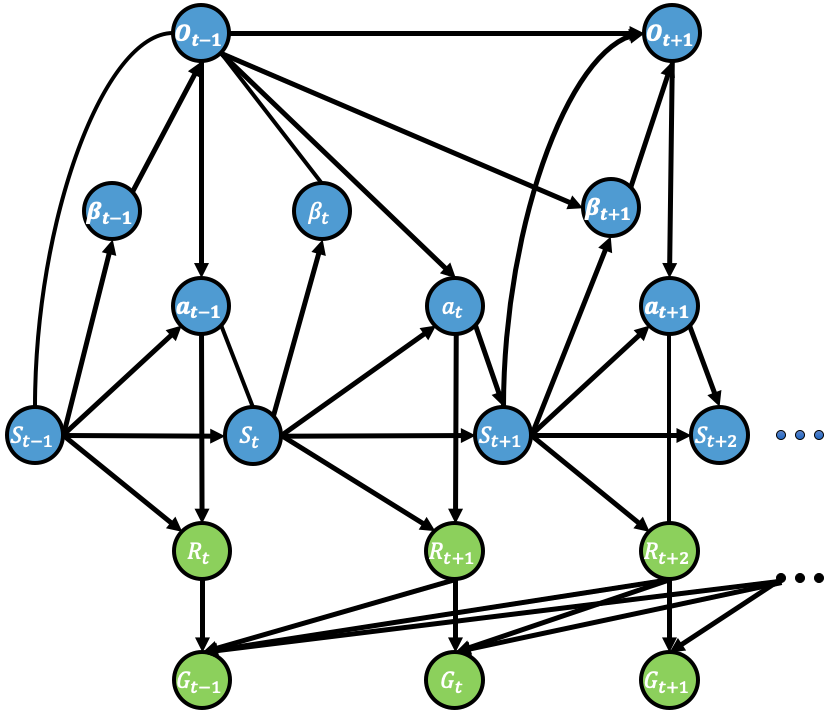
\includegraphics[width=0.5\linewidth]{figures/oc_smdp.png}\\
%   \caption{\label{fig:oc_smdp} An Illustration of the SMDP Option
%     Framework. An option $\ro_{t-1}$ is selected by
%     master policy $P(\ro_{t-1}|\rvs_{t-1})$ at time step
%     $t-1$. At time step $t$, \emph{termination function}
%     $\beta_{o_{t-1}}(\rvs_t)$ determines to continue option
%     $\ro_{t-1}$. So that there is no random variable $\ro_t$ at
%     time step $t$ compared to there are random variables $\rvo$
%     at every time step in MDP formulation
%     (figure~\ref{fig:oc_pgm}).}
% \end{figure*}
% Due to the SMDP formulation, an option can only be improved when
% the option terminates. We refer this as the SMDP-style learning
% which is sample inefficient and prevents applying SOTA MDP based
% algorithms such as the Proximal Policy Optimization (PPO)
% algorithm \cite{schulman2017proximal}.



% \subsection{HMM dynamics for the Option Framework}
% \label{sec:appen_hmm}

% We follow \citename{bishop2006pattern}'s formulation of mixture
% distribution and Probabilistic Graphical Models (PGMs). By
% introducing option variables as latent variables and adding extra
% dependencies between them, we show that the conventional SMDP
% version of the option framework
% \cite{bacon2017option,sutton2018reinforcement,sutton1999between,harb2018waiting,zhang2019dac}
% has an MDP equivalence.
% \begin{figure*}[th!]
%   \centering
%   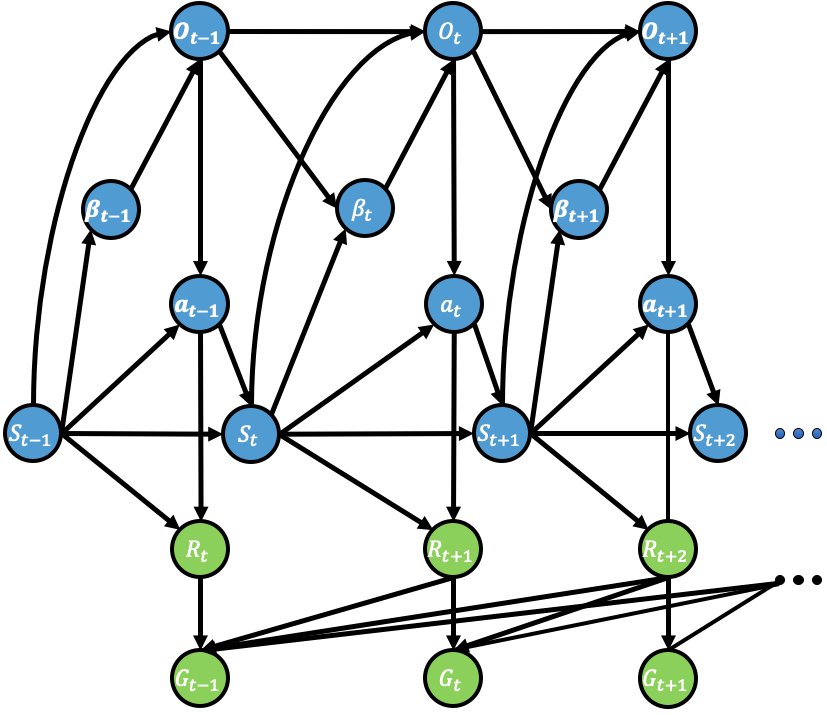
\includegraphics[width=0.5\linewidth]{figures/oc_pgm.png}\\
%   \caption{\label{fig:oc_pgm} PGM of the MDP Option Framework}
% \end{figure*}
% Following \citet{bishop2006pattern}'s notation, we use bolded
% letter $\rvs\in\sS$ to denote a random variable and normal letter
% $\rs$ to denote its realization. Without special clarification, a
% random vector can have either a vector of continuous or discrete
% entries. Vector $\rvo\in\sO$ is an $M$-dimensional one-hot vector
% and each entry $\ro\in\{0,1\}$ is a binary random variable.
% $P(\rvo_t|\rvs_t)$ denotes the probability distribution over
% one-hot vector $\rvo$ at time step $t$ conditioned on state
% $\rvs_t$. $P(\rvo_t=\ro_t|\rvs_t)$ denotes a probability entry (a
% scalar value) of the random variable $\rvo_t$ with a realization
% at time step $t$ where $\ro_t=1$ and $\ro\in\rvo_t/\ro_t=0$.
% % todo: define an option set P_o(a) P_o(b) I

% In figure~\ref{fig:oc_pgm}, $\rvs\in\sS$, $\rvo\in\sO^M$,
% $\rvb\in\sB^M$ and $\rva \in \sA$, denote the state, option,
% termination and action random variable respectively. $\rvo$ is an
% $M$-dimensional one-hot vector and $\rvb$ is an $M$-dimensional
% binary vector where each entry $\rb\in\{0,1\}$. $M$ is the number
% of options. $R_{t+1}$ is the actual reward received from the
% environment after executing action $\rva_{t}$ in state $\rvs_t$.
% $G_t=R_{t+1}+\gamma R_{t+2}+\gamma^2R_{t+3}\cdots$ is the
% discounted expected return where $\gamma\in \sR$ is a discount
% factor.

% The termination policy distribution
% $P(\rvb_t|\rvs_t,\rvo_{t-1}):\sS\times\sO\rightarrow\sB$ can be
% formulated as a mixture distribution\footnote{Different from
%   conventional formulation which only depends on state $\rvs_t$,
%   our \emph{termination function} has an extra dependence on
%   $\rvo_{t-1}$} conditioned on option vector (the one-hot vector)
% $\rvo_{t-1}$ and state $\rvs_t$.
% \begin{equation}
%   \label{eq:oc_beta_p}
% P(\rvb_t|\rvs_t,\rvo_{t-1}) = \prod_{\ri\in\rvo_{t-1}}P_{\ri}(\rb_t|\rvs_t)^{\ri}.
% \end{equation}

% Because each option has its own \textbf{termination policy}
% $P_o(\rvb|\rvs)$, with a slightly abuse of notation, in
% equation~(\ref{eq:oc_beta_p}) we use
% $P(\rvb_t|\rvs_t,\rvo_{t-1})$ to denote the termination policy
% activated at time step $t$ by previous chosen option
% $\rvo_{t-1}$. To keep notation uncluttered, we use
% $\beta_t=P(\rvb_t=1|\rvs_t,\rvo_{t-1})$ to denote the probability
% of option $\rvo_{t-1}$ terminates at time step $t$ and
% $(1-\beta_t) = P(\rvb_t=0|\rvs_t,\rvo_{t-1})$ to denote the
% probability of continuation.

% Conventionally, master policy \cite{zhang2019dac} (also called
% ``policy-over-options''~\cite{sutton1999between,bacon2017option}))
% is defined as:
% \begin{equation}
%   \label{eq:oc_master}
%   P(\rvo_t|\rvs_t).
% \end{equation}
% Similarly, we propose a novel \textbf{mixture master policy} as a
% mixture distribution\footnote{Different from conventional
%   formulation which only depends on state $\rvs_t$, our mixture
%   master policy has extra dependencies on $\rvo_{t-1}$ and
%   $\rvb_t$}:

% \begin{equation}
%   \label{eq:oc_po}
% P(\rvo_t|\rvs_t, \rvb_t,\rvo_{t-1}) = P(\rvo_t|\rvs_t)^{\rb_t}P(\rvo_t|\rvo_{t-1})^{1-\rb_t},
% \end{equation}
% ~where $P(\rvo_t|\rvo_{t-1})$ is a degenerate probability
% distribution~\cite{puterman2014markov}

% \begin{equation}
%   \label{eq:deg_puterman}
% P(\rvo_t|\rvo_{t-1}) = 
% \begin{cases}
%   1&\;\text{if } \rvo_t=\rvo_{t-1},\\
%   0&\;\text{if } \rvo_t\neq\rvo_{t-1}.
% \end{cases}
% \end{equation}

% As shown in equation~(\ref{eq:oc_po}), the master policy only
% exists when $\rb_t=1$ the option terminates. Therefore, PPOC
% \cite{klissarov2017learnings} uses inaccurate gradients for
% updating the master policy during an option's execution.

% According to the conditional dependency relationships in PGM
% (figure~\ref{fig:oc_pgm}), the joint probability distribution of
% $\rvo_t$ and $\rvb_t$ can be written as:
% \begin{equation}
%   \label{eq:oc_ob_p}
%   P(\rvo_t,\rvb_t|\rvs_t,\rvo_{t-1})=P(\rvb_t|\rvs_t,\rvo_{t-1})P(\rvo_t|\rvs_t, \rvb_t,\rvo_{t-1}),
% \end{equation}
% ~and the marginal probability distribution can be written as:
% \begin{align}
%   \label{eq:oc_oso_p}
%   P(\rvo_t|\rvs_t,\rvo_{t-1})&=\sum_{\rvb_t}P(\rvb_t|\rvs_t,\rvo_{t-1})P(\rvo_t|\rvs_t, \rvb_t,\rvo_{t-1})\\
%   \nonumber &=P(\rvb_t=0|\rvs_t,\rvo_{t-1})P(\rvo_t|\rvo_{t-1}) +P(\rvb_t=1|\rvs_t,\rvo_{t-1})P(\rvo_t|\rvs_t) \\
% \nonumber                             &=(1-\beta_t)P(\rvo_t|\rvo_{t-1}) +\beta_tP(\rvo_t|\rvs_t)\\
%   \nonumber&=(1-\beta_t)\1_\mathrm{\rvo_t=\rvo_{t-1}} +\beta_tP(\rvo_t|\rvs_t).
% \end{align}

% The \textbf{intra-option (action) policy} distribution can also
% be formulated as a mixture distribution
% \begin{equation}
%   \label{eq:oc_a_p}
%   P(\rva_t|\rvs_t,\rvo_t) = \prod_{\ri\in\rvo_t}P_{\ri}(\rva_t|\rvs_t)^{\ri}.
% \end{equation}
% Therefore, the dynamics of the PGM in
% figure~\ref{fig:oc_pgm} can be written as:
% \begin{align}
%   \label{eq:app_oc_pgm_joint}
%   \nonumber  P(\tau) = &P(\rvs_0)P(\rvo_0)P(\rva_0|\rvs_0,\rvo_0)\\
%                        &\prod_{t=1}^\infty P(\rvs_t|\rvs_{t-1},\rva_{t-1})P(\rva_{t}|\rvs_{t},\rvo_{t})\sum_{\rvb_t}P(\rvb_t|\rvs_t,\rvo_{t-1})P(\rvo_t|\rvb_t,\rvs_t,\rvo_{t-1})\\
%   = &P(\rvs_0)P(\rvo_0)P(\rva_0|\rvs_0,\rvo_0)
%       \prod_{t=1}^\infty P(\rvs_t|\rvs_{t-1},\rva_{t-1})P(\rva_{t}|\rvs_{t},\rvo_{t})P(\rvo_t|\rvs_t,\rvo_{t-1}),
% \end{align}
% ~where
% $P(\tau)=P(\rvs_0,\rvo_0,\rva_0,\rvs_1,\rvb_1,\rvo_1,\rva_1,\ldots)$
% denotes the joint distribution of the PGM. Notice that under this
% formulation, $P(\tau)$ is actually an HMM with $\rvs_t$, $\rva_t$
% as observable random variables and $\rvb_t$, $\rvo_t$ as latent
% variables.

% It is worth to mention that equation~(\ref{eq:deg_puterman}) is
% essentially the indicator function
% $\1_\mathrm{\rvo_t=\rvo_{t-1}}$ used in conventional SMDP option
% framework papers and the last line in
% equation~(\ref{eq:oc_oso_p}) is identical to transitional
% probability distribution in their formulation. However, as we
% show in this section, by adding latent variables $\rvo_{t-1}$ and
% introducing the dependency between $\rvo_{t}$ and $\rvb_t$, our
% formulation is essentially an HMM. It
% % todo: contribution
% opens the door to introduce many well developed PGM algorithms
% such as message passing~\cite{forney1973viterbi} and variational
% inference~\cite{hoffman2013stochastic} to the reinforcement
% learning framework. As we show below, the nice conditional
% independence relationships enjoyed by this model also enable us
% to prove the equivalence between the option framework's SMDP and
% MDP formulation.

% \subsection{MDP formulation for the Option Framework}
% \label{sec:appen_mdp}

% With PGM in hand, we now prove that the HMM formulated MDP option
% framework has identical value functions with the conventional
% SMDP option framework\cite{bacon2017option,sutton1999between}. In
% this section, we first show that all value functions defined on
% our PGM are identical to the SMDP formulation. We will prove that
% the gradients are also the same in next section.

% We follow \citename{sutton2018reinforcement}'s notation in this
% section and write value functions for MDP below:

% \begin{align}
%   \label{eq:oc_v}
%   \nonumber  V[\rvs_t] &= \E[G_t|\rvs_t] = \sum_{G_t}G_t\sum_{\rvo_t}P(G_t,\rvo_t|\rvs_t)\\
%   \nonumber  &= \sum_{\rvo_t}P(\rvo_t|\rvs_t)\sum_{G_t}G_tP(G_t|\rvs_t, \rvo_t)\\
%   \nonumber  &= \sum_{\rvo_t}P(\rvo_t|\rvs_t)\E[G_t|\rvo_t, \rvs_t]\\
%   &=\sum_{\rvo_t}P(\rvo_t|\rvs_t)Q_{O}[\rvo_t,\rvs_t],
% \end{align}
% ~where $V[\rvs_t]$ is the state value
% function\cite{sutton2018reinforcement} and $Q_O[\rvo_t,\rvs_t]$
% is the option value
% function\cite{bacon2017option,sutton1999between}. Note that in
% deriving equation~(\ref{eq:oc_v}) we only use summation rule and
% production rule, the conditional dependency relationships in PGM
% (figure~\ref{fig:oc_pgm}) are not used. The option value function
% $Q_O[\rvo_t,\rvs_t]$ can be further expanded as:
% \begin{align}
%   \label{eq:oc_qos}
%   \nonumber  Q_O[\rvo_t,\rvs_t] &= \E[G_t|\rvo_t, \rvs_t] = \sum_{\rva_t}P(\rva_t|\rvs_t,\rvo_t)\E[G_t|\rvo_t, \rvs_t,\rva_t]\\
% &= \sum_{\rva_t}P(\rva_t|\rvs_t,\rvo_t)Q_U[\rvo_t, \rvs_t,\rva_t],
% \end{align}
% ~where $Q_U[\rvo_t, \rvs_t,\rva_t]$ is the option-action value
% function.

% \begin{prop}
%   \label{prop:oc_q_soa}
%   MDP formulation has identical state value function $V[\rvs_t]$
%   and option value function $Q_O[\rvo_t,\rvs_t]$ to SMDP
%   formulations
% \end{prop}

% \begin{proof}
%   Note that in derivations above we only use summation and
%   production rules. Both equation~(\ref{eq:oc_v})
%   and~(\ref{eq:oc_qos}) are identical to the conventional SMDP
%   option framework.
% \end{proof}

% From now on, we will continue derivations with conditonal
% independence relationships encoded in PGM (Chapter 8.2.1
% \cite{bishop2006pattern}). We have following conditional
% independence relationships from PGM (figure~\ref{fig:oc_pgm}):

% \begin{align}
% \label{eq:c1}  \{R_{t+2},G_{t+1}\}&\bigCI \{\rvb_{t+1}\} &|\;&\{\rvo_{t+1}\},\\
% \label{eq:c2} \{R_{t+2},G_{t+1}\}&\bigCI \{\rvs_t\} &|\;&\{\rvs_{t+1},\rvo_t\},\\
% \label{eq:c3}  \{R_{t+2},G_{t+1}\}&\bigCI \{\rva_t\} &|\;&\{\rvs_{t+1}\},\\
% \label{eq:c4}  \{R_{t+2},G_{t+1}\}&\bigCI \{\rvo_t\} &|\;&\{\rvs_{t+1},\rvo_{t+1}\},\\
% \label{eq:c5}  \{R_{t+1},G_{t},\rvs_{t+1}\}&\bigCI \{\rvo_t\} &|\;&\{\rva_{t}\}.
% \end{align}

% With above conditional independence relationships in hand, we now
% show that the MDP formulation has identical value functions to
% the conventional SMDP
% formulation\cite{sutton1999between,bacon2017option}.

% \begin{prop}
%   \label{prop:oc_q_soa}
%   MDP formulation has identical option-action value function
%   $Q_U[\rvo_t, \rvs_t,\rva_t]$ to SMDP formulations
% \begin{equation}
%   \label{eq:oc_q_soa}
%   Q_U[\rvo_t, \rvs_t,\rva_t]=r(\rvs_t,\rva_t)+\gamma\sum_{\rvs_{t+1}}P(\rvs_{t+1}|\rvs_t,\rva_t)U[\rvs_{t+1},\rvo_t].
% \end{equation}
% \end{prop}

% \begin{proof}
% \begin{align*}
%   Q_U[\rvo_t, \rvs_t,\rva_t] = &\E[G_t|\rvo_t, \rvs_t,\rva_t] &\text{\;} \\
%   = &\E[R_{t+1}+\gamma G_{t+1}|\rvo_t, \rvs_t,\rva_t] & \text{by definition of $G_t$}\\
%   =&\E[R_{t+1}|\rvs_t,\rva_t] +&\text{use eq~(\ref{eq:c5})} \\
%                                &\gamma\sum_{G_{t+1}}G_{t+1}\sum_{\rvs_{t+1}}P(\rvs_{t+1}|\rvs_t,\rvo_t,\rva_t)P(G_{t+1}|\rvs_{t+1},\rvo_t,\rvs_t,\rva_t)\\
%   =&r(\rvs_t,\rva_t)+\\
%                                &\gamma\sum_{G_{t+1}}G_{t+1}\sum_{\rvs_{t+1}}P(\rvs_{t+1}|\rvs_t,\rva_t)P(G_{t+1}|\rvs_{t+1},\rvo_t) &\text{use eq~\ref{eq:c2}~\ref{eq:c3} and ~\ref{eq:c5}}\\
%   =&r(\rvs_t,\rva_t)+\gamma\sum_{\rvs_{t+1}}P(\rvs_{t+1}|\rvs_t,\rva_t)\E[ G_{t+1}|\rvs_{t+1},\rvo_t ]\\
%   =&r(\rvs_t,\rva_t)+\gamma\sum_{\rvs_{t+1}}P(\rvs_{t+1}|\rvs_t,\rva_t)U[\rvs_{t+1},\rvo_t].
% \end{align*}
% \end{proof}


% \begin{prop}
%   \label{prop:oc_u}
%   MDP formulation has identical option-value function upon
%   arrival $U[\rvs_{t+1},\rvo_t]$ to SMDP
%   formulations\footnote{Both equations~(\ref{eq:oc_u_qv})
%     and~(\ref{eq:oc_u_qa}) is largely used in the conventional
%     SMDP papers\cite{sutton1999between,bacon2017option}.}
%  \begin{align}
% \label{eq:oc_u_qv}  U[\rvs_{t+1},\rvo_t]= &(1-\beta_{t+1})Q_O[\rvo_{t+1}=\ro_t,\rvs_{t+1}] +\beta_{t+1}V[\rvs_{t+1}]\\
%  \label{eq:oc_u_qa} = &Q_O[\rvo_{t+1}=\ro_t,\rvs_{t+1}] -\beta_{t+1}A[\rvo_{t+1}=\ro_t,\rvs_{t+1}].
% \end{align}
% \end{prop}


% \begin{proof}
%  \begin{align*}
%   U[\rvs_{t+1},\rvo_t]=&\E[ G_{t+1}|\rvs_{t+1},\rvo_t ]\\
%   =&\sum_{G_{t+1}}G_{t+1}\\
%                        &\sum_{\rvo_{t+1}}\sum_{\rvb_{t+1}}P(\rvb_{t+1}|\rvo_t,\rvs_{t+1})P(\rvo_{t+1}|\rvb_{t+1},\rvo_t,\rvs_{t+1})P(G_{t+1}|\rvo_{t+1},\rvb_{t+1},\rvo_t,\rvs_{t+1})\\
%   =&\sum_{\rvo_{t+1}}\sum_{\rvb_{t+1}}P(\rvb_{t+1}|\rvo_t,\rvs_{t+1})P(\rvo_{t+1}|\rvb_{t+1},\rvo_t,\rvs_{t+1})\sum_{G_{t+1}}G_{t+1}P(G_{t+1}|\rvo_{t+1},\rvs_{t+1})\\
%   = &\sum_{\rvo_{t+1}}\big[(1-\beta_{t+1})\1_\mathrm{\rvo_{t+1}=\rvo_t} +\beta_{t+1}P(\rvo_{t+1}|\rvs_{t+1})\big]Q_O[\rvo_{t+1},\rvs_{t+1}]\\
%   = &(1-\beta_{t+1})Q_O[\rvo_{t+1}=\ro_t,\rvs_{t+1}] +\beta_{t+1}V[\rvs_{t+1}]\\
%   = &Q_O[\rvo_{t+1}=\ro_t,\rvs_{t+1}] -\beta_{t+1}A[\rvo_{t+1}=\ro_t,\rvs_{t+1}].
% \end{align*}
% ~from line 3 to line 4 use equation (\ref{eq:c1}) and
% (\ref{eq:c4}). From line 4 to line 5 use equation
% (\ref{eq:oc_oso_p}) and definition of $Q_O$. The second last line
% use equation~(\ref{eq:oc_v}). The last line use the definition of
% advantage function $A$.
% \end{proof}

% Under our MDP formulation, we also propose proposition
% \ref{approp:oc_u_pgm}. We derive our gradient theorems based on
% equation~(\ref{eq:oc_u_pgm}) in section~\ref{sec:appen_mdp_grad}.
% This important relationship largely simplify derivations than the
% original paper~\cite{bacon2017option} as well as give rise to the
% O2V.

% \begin{prop}
%     \label{approp:oc_u_pgm}
%     The option-value function upon arrival $U[\rvs_{t+1},\rvo_t]$
%     is an expectation over option value function
%     $Q_O[\rvo_{t+1},\rvs_{t+1}]$ conditioned on previous option
%     $O_{t}$
%   \begin{equation}
%     \label{eq:oc_u_pgm}
%     U[\rvs_{t+1},\rvo_t]= \sum_{\rvo_{t+1}}P(\rvo_{t+1}|\rvo_t,\rvs_{t+1})Q_O[\rvo_{t+1},\rvs_{t+1}].
%   \end{equation}
% \end{prop}

% \begin{proof}
%   Following proof of proposition \ref{prop:oc_u},
%  \begin{align*}
%   \nonumber U[\rvs_{t+1},\rvo_t]=&\sum_{\rvo_{t+1}}\sum_{\rvb_{t+1}}P(\rvb_{t+1}|\rvo_t,\rvs_{t+1})P(\rvo_{t+1}|\rvb_{t+1},\rvo_t,\rvs_{t+1})\sum_{G_{t+1}}G_{t+1}P(G_{t+1}|\rvo_{t+1},\rvs_{t+1})\\
% =&\sum_{\rvo_{t+1}}P(\rvo_{t+1}|\rvo_t,\rvs_{t+1})Q_O[\rvo_{t+1},\rvs_{t+1}].
% \end{align*}
% \end{proof}

% \subsection{Gradients for the MDP Option Framework}
% \label{sec:appen_mdp_grad}

% In above sections, we formulate dynamics of the option framework
% using HMM and prove the MDP build on it has identical value
% functions to SMDP formulation. In this section we will prove that
% both MDP and SMDP formulations~\cite{bacon2017option} share same
% intra-option and termination gradients. Our derivations is
% largely simplified by equation~(\ref{eq:oc_u_pgm}) compared to
% previous work.

% Let $\theta_a$ denote parameter vector for intra-option policies
% $P(\rva_t|\rvs_t,\rvo_t;\theta_a)$ and $\theta_b$ denote
% parameter vector for termination policies
% $P(\rvb_t|\rvs_t,\rvo_{t-1};\theta_b)$. To keep notation
% uncluttered, we drop the dependency on parameter vector $\theta$
% in derivations below.

% \begin{prop}
%   \label{approp:oc_a_grad}
%   MDP formulation has identical Intra-Option Policy Gradient with
%   SMDP formulation in~\cite{bacon2017option}.
%   \begin{align}
%     \nonumber    \frac{\partial Q_O[ \rvs_t,\rvo_t ]}{\partial \theta_a}=
%     \sum_{\rk=0}^\infty&\sum_{\rvs_{t+k},\rvo_{t+k}}P_\gamma^{(k)}(\rvs_{t+k},\rvo_{t+k}|\rvs_t,\rvo_t)\\
%     \label{eq:oc_a_grad}    &\sum_{\rva_{t+k}}\frac{\partial P(\rva_{t+k}|\rvs_{t+k},\rvo_{t+k})}{\partial \theta_a}Q_U(\rvs_{t+k},\rvo_{t+k},\rva_{t+k}).
%   \end{align}
% \end{prop}

% \begin{proof}
%   This is a direct result by taking gradient of $\theta_a$ with
%   respect to equation~(\ref{eq:oc_qos}) by using
%   equation~(\ref{eq:oc_q_soa}) and (\ref{eq:oc_u_pgm}):
% \begin{align*}
%   \frac{\partial Q_O[ \rvs_t,\rvo_t ]}{\partial \theta_a}=&\sum_{\rva_t}\frac{\partial P(\rva_t|\rvs_t,\rvo_t)}{\partial \theta_a}Q_U[\rvo_t, \rvs_t,\rva_t]+\gamma\sum_{\rva_t}P(\rva_t|\rvs_t,\rvo_t)\frac{\partial Q_U[\rvo_t, \rvs_t,\rva_t]}{\partial \theta_a}\\
%   =&\sum_{\rva_t}\frac{\partial P(\rva_t|\rvs_t,\rvo_t)}{\partial \theta_a}Q_U[\rvo_t, \rvs_t,\rva_t]\\
%                                                         &+ \gamma\sum_{\rva_t}P(\rva_t|\rvs_t,\rvo_t)\sum_{\rvs_{t+1}}P(\rvs_{t+1}|\rvs_t,\rva_t)\frac{\partial U[\rvo_t,\rvs_{t+1}]}{\partial \theta_a}\\
%   =&\sum_{\rva_t}\frac{\partial P(\rva_t|\rvs_t,\rvo_t)}{\partial \theta_a}Q_U[\rvo_t, \rvs_t,\rva_t]\\
%                                                         &+ \gamma\sum_{\rvs_{t+1}}P(\rvs_{t+1}|\rvs_t,\rvo_t)\sum_{\rvo_{t+1}}P(\rvo_{t+1}|\rvs_{t+1},\rvo_t)\frac{\partial Q_O[\rvo_{t+1},\rvs_{t+1}]}{\partial \theta_a}\\
%   =&\sum_{\rva_t}\frac{\partial P(\rva_t|\rvs_t,\rvo_t)}{\partial \theta_a}Q_U[\rvo_t, \rvs_t,\rva_t] + \gamma\sum_{\rvo_{t+1},\rvs_{t+1}}P(\rvs_{t+1},\rvo_{t+1}|\rvs_{t},\rvo_t)\frac{\partial Q_O[\rvo_{t+1},\rvs_{t+1}]}{\partial \theta_a}\\
%   =&\sum_{\rk=0}^\infty\sum_{\rvs_{t+k},\rvo_{t+k}}P_\gamma^{(k)}(\rvs_{t+k},\rvo_{t+k}|\rvs_t,\rvo_t)\\
%                                                         &\sum_{\rva_{t+k}}\frac{\partial P(\rva_{t+k}|\rvs_{t+k},\rvo_{t+k})}{\partial \theta_a}Q_U(\rvs_{t+k},\rvo_{t+k},\rva_{t+k}).
% \end{align*}
% \end{proof}

% \begin{prop}
%   \label{approp:oc_b_grad}
%   MDP formulation has identical Termination Policy Gradient with
%   SMDP formulation in~\cite{bacon2017option}.
%   \begin{align}
%     \label{eq:oc_b_grad}   \frac{\partial U[ \rvs_{t+1},\rvo_t ]}{\partial \theta_b}=
%     -\sum_{\rk=0}^\infty&\sum_{\rvs_{t+1+k},\rvo_{t+k}}P_\gamma^{(k)}(\rvs_{t+1+k},\rvo_{t+k}|\rvs_{t+1},\rvo_t)
%                          \frac{\partial \beta_{t+1+k}}{\partial \theta_b}A[ \rvs_{t+k+1},\rvo_{t+k+1}=\rvo_{t+k}].
%   \end{align}
% \end{prop}

% \begin{proof}
%   We first show the gradient of $\theta_b$ with respect to
%   equation~(\ref{eq:oc_oso_p}) and (\ref{eq:oc_qos}) separately:

%   \begin{align}
%     \label{eq:oc_oso_p_grad} \frac{\partial P(\rvo_{t+1}|\rvs_{t+1},\rvo_{t})}{\partial \theta_b} = &\big[P(\rvo_{t+1}|\rvs_{t+1})-\1_\mathrm{\rvo_t=\rvo_{t-1}}\big]\frac{\partial \beta_{t+1}}{\partial \theta_b}\\
%     \nonumber\frac{\partial Q_O[\rvo_{t+1},\rvs_{t+1}]}{\partial \theta_b} =& \sum_{\rva_{t+1}}P(\rva_{t+1}|\rvs_{t+1},\rvo_{t+1})\sum_{\rvs_{t+2}}P(\rvs_{t+2}|\rvs_{t+1},\rva_{t+1})\frac{\partial U[\rvs_{t+2},\rvo_{t+1}]}{\partial \theta_b}\\
%  \label{eq:oc_qos_grad}   =&\sum_{\rvs_{t+2}}P(\rvs_{t+2}|\rvs_{t+1},\rvo_{t+1})\frac{\partial U[\rvs_{t+2},\rvo_{t+1}]}{\partial \theta_b}.
%   \end{align}

%   The equation~(\ref{eq:oc_b_grad}) is a direct result by taking
%   gradient of $\theta_b$ with respect to
%   equation~(\ref{eq:oc_u_pgm}) and using above results:
%   \begin{align*}
%     \frac{\partial U[ \rvs_{t+1},\rvo_t ]}{\partial \theta_b}=&\sum_{\rvo_{t+1}}\frac{\partial P(\rvo_{t+1}|\rvo_t,\rvs_{t+1})}{\partial \theta_b}Q_O[\rvo_{t+1},\rvs_{t+1}] + \sum_{\rvo_{t+1}}P(\rvo_{t+1}|\rvo_t,\rvs_{t+1})\frac{\partial Q_O[\rvo_{t+1},\rvs_{t+1}]}{\partial \theta_b}\\
%     =&\sum_{\rvo_{t+1}} \big[P(\rvo_{t+1}|\rvs_{t+1})-\1_\mathrm{\rvo_t=\rvo_{t-1}}\big]Q_O[\rvo_{t+1},\rvs_{t+1}]\frac{\partial \beta_{t+1}}{\partial \theta_b}\\
%     &+\sum_{\rvo_{t+1}}P(\rvo_{t+1}|\rvo_t,\rvs_{t+1})\gamma\sum_{\rvs_{t+2}}P(\rvs_{t+2}|\rvs_{t+1},\rvo_{t+1})\frac{\partial U[\rvs_{t+2},\rvo_{t+1}]}{\partial \theta_b}\\
%     =& \big[V[ \rvs_{t+1} ]-Q_O[\rvo_{t+1}=\rvo_t,\rvs_{t+1}]\big]\frac{\partial \beta_{t+1}}{\partial \theta_b}\\
%     &+\gamma\sum_{\rvo_{t+1},\rvs_{t+2}}P(\rvs_{t+2},\rvo_{t+1}|\rvs_{t+1},\rvo_{t})\frac{\partial U[\rvs_{t+2},\rvo_{t+1}]}{\partial \theta_b}\\
%     =& -A[\rvo_{t+1}=\rvo_t,\rvs_{t+1}]\frac{\partial \beta_{t+1}}{\partial \theta_b}+\gamma\sum_{\rvo_{t+1},\rvs_{t+2}}P(\rvs_{t+2},\rvo_{t+1}|\rvs_{t+1},\rvo_{t})\frac{\partial U[\rvs_{t+2},\rvo_{t+1}]}{\partial \theta_b}\\
%     =&-\sum_{\rk=0}^\infty\sum_{\rvs_{t+1+k},\rvo_{t+k}}P_\gamma^{(k)}(\rvs_{t+1+k},\rvo_{t+k}|\rvs_{t+1},\rvo_t)
%                          \frac{\partial \beta_{t+1+k}}{\partial \theta_b}A[ \rvs_{t+k+1},\rvo_{t+k+1}=\rvo_{t+k}].
%   \end{align*}
  
% \end{proof}
% \newpage
% \section{Derivations of the Option2Vec architecture's value
%   functions}
% \label{sec:appen_sa_v_proof}

% Following \citename{bishop2006pattern}'s notation, we use $A$,
% $B$ and $C$ to denote three non-overlapping sets of arbitrarily
% many random variables. Sets $A$ and $B$ are conditional
% independent on set $C$ if $P(A,B|C)=P(A|C)P(B|C)$, denoted as
% $A\bigCI B \;|\; C$. We mainly use head-to-tail conditional
% independence properties (Chapter 8.2.1 \cite{bishop2006pattern})
% in this section.

% Derivations of Eq.~(\ref{eq:sa_v}):
% \begin{align*}
%   V[\rvs_t,\hat{\rvo}_{t-1}]=&\E[G_t|\rvs_t,\hat{\rvo}_{t-1}]\\
%   =& \sum_{\hat{\rvo}_t}P(\hat{\rvo}_t|\rvs_t,\hat{\rvo}_{t-1})\E(G_t|\rvs_t,\hat{\rvo}_t,\hat{\rvo}_{t-1})\\
%   =& \sum_{\hat{\rvo}_t}P(\hat{\rvo}_t|\rvs_t,\hat{\rvo}_{t-1})\E[ G_t|\rvs_t,\hat{\rvo}_t ]\\
%   =& \sum_{\hat{\rvo}_t}P(\hat{\rvo}_t|\rvs_t,\hat{\rvo}_{t-1})Q_O[ \hat{\rvo}_t,\rvs_t],
% \end{align*}

% ~where from line 2 to line 3 we use the conditional independence
% property in PGM that $G_t\bigCI\hat{\rvo}_{t-1}|\{\rvs_t,\hat{\rvo}_t\}$.
% \begin{proof}
%  for Proposition~\ref{prop:var_unb}: By law of total expectation:

%   $$\E_{\hat{\rvo}_{t-1}}[V[\rvs_t,\hat{\rvo}_{t-1}]]=\E_{\hat{\rvo}_{t-1}}[\E[G_t|\rvs_t,\hat{\rvo}_{t-1}]]=\E[G_t|\rvs_t] = V[\rvs_t]$$

% thus $V[\rvs_t,\hat{\rvo}_{t-1}]$ is an unbiased estimator of $V[\rvs_t]$.
% \end{proof}

% \begin{proof}
%   for Proposition~\ref{prop:var_red}: By law of total conditional
%   variance:
% \begin{align*}
%   \text{Var}(V[\rvs_t]) &= \text{Var}([\E[G_t|\rvs_t]]) =\E[\text{Var}(\E[G_t|\rvs_t,\hat{\rvo}_{t-1}])|\rvs_t]+\text{Var}(\E[\E[G_t|\rvs_t,\hat{\rvo}_{t-1}]]|\rvs_t)\\
%                         &= \E[\text{Var}(V[\rvs_t,\hat{\rvo}_{t-1}])|\rvs_t]+\text{Var}(\E[V[\rvs_t,\hat{\rvo}_{t-1}]]|\rvs_t)\\
%   &\geq \text{Var}(\E[V[\rvs_t,\hat{\rvo}_{t-1}]]|\rvs_t).
% \end{align*}
% \end{proof}

% Derivations of Eq.~(\ref{eq:sa_q_a})
% \begin{align*}
%   Q_A[ \rvs_t,\hat{\rvo}_t,\rva_t]=&\E[G_t| \rvs_t,\hat{\rvo}_t,\rva_t]
%                                =\E[R_{t+1}+\gamma G_{t+1}| \rvs_t,\hat{\rvo}_t,\rva_t]\\
%   =& r(s,o,a) + \gamma\sum_{\rvs_{t+1}}P(\rvs_{t+1}|\rvs_t,\hat{\rvo}_t,\rva_t)\E[G_{t+1}|\rvs_{t+1},\rvs_t,\hat{\rvo}_t,\rva_t]\\
%   =& r(s,a) + \gamma\sum_{\rvs_{t+1}}P(\rvs_{t+1}|\rvs_t,\rva_t)\E[G_{t+1}|\rvs_{t+1},\hat{\rvo}_t]\\
%   =& r(s,a) + \gamma\sum_{\rvs_{t+1}}P(\rvs_{t+1}|\rvs_t,\rva_t)V[\rvs_{t+1},\hat{\rvo}_t],
% \end{align*}

% ~where from line 2 to line 3 we use the conditional independence
% property in PGM that $R_{t+1}\bigCI\hat{\rvo}_{t}|\rva_t$,
% $G_{t+1}\bigCI\rvs_{t}|\{\rvs_{t+1},\hat{\rvo}_t\}$ and
% $G_{t+1}\bigCI\rva_{t}|\rvs_{t+1}$. $\gamma \in \sR$ is a
% discounting factor.


% \section{Proofs for the Option2Vec architecture gradient
%   theorems}
% \label{sec:appen_sa_proof}

% \subsection{Proof for the skill policy gradient theorem}
% \label{sec:appen_sa_o_grad}

% \begin{proof}
%     \begin{align*}
%       \frac{\partial Q_O[\rvs_t,\hat{\rvo}_t]}{ \partial \theta_o }=& \sum_{\rva_t}P(\rva_t|\rvs_t,\hat{\rvo}_t)\big[r(s,a) + \gamma\sum_{\rvs_{t+1}}P(\rvs_{t+1}|\rvs_t,\rva_t)\frac{\partial V[\rvs_{t+1},\hat{\rvo}_t]}{\partial \theta_o}\big]\\
%       =&\sum_{\rvs_{t+1}}\gamma P(\rvs_{t+1}|\rvs_t,\hat{\rvo}_t)\frac{\partial V[\rvs_{t+1},\hat{\rvo}_t]}{\partial \theta_o}\\
%       \frac{\partial V[\rvs_t,\hat{\rvo}_{t-1}]}{\partial \theta_o}=&\sum_{\hat{\rvo}_t}\frac{\partial P(\hat{\rvo}_t|\rvs_t,\hat{\rvo}_{t-1})}{\partial \theta_o}Q_O[\rvs_t,\hat{\rvo}_t]+\gamma\sum_{\hat{\rvo}_t}P(\hat{\rvo}_t|\rvs_t,\hat{\rvo}_{t-1})\frac{Q_O[\rvs_t,\hat{\rvo}_t]}{\partial \theta_o}\\
%       =&\sum_{\hat{\rvo}_t}\frac{\partial P(\hat{\rvo}_t|\rvs_t,\hat{\rvo}_{t-1})}{\partial \theta_o}Q_O[\rvs_t,\hat{\rvo}_t]
%          +\gamma\sum_{\rvs_{t+1},\hat{\rvo}_t}P(\rvs_{t+1},\hat{\rvo}_t|\rvs_t,\hat{\rvo}_{t-1})\frac{\partial V[\rvs_{t+1},\hat{\rvo}_t]}{\partial \theta_o}\\
%       =&-\sum_{\rk=0}^\infty\sum_{\rvs_{t+k},\hat{\rvo}_{t+k-1}}\\
%                                                               &P_{\gamma}^{(k)}(\rvs_{t+k},\hat{\rvo}_{t+k-1}|\rvs_{t},\hat{\rvo}_{t-1})\sum_{\hat{\rvo}_{t+k}}\frac{\partial P(\hat{\rvo}_{t+k}|\rvs_{t+k},\hat{\rvo}_{t+k-1})}{\partial \theta_o}Q_O[ \rvs_{t+k},\hat{\rvo}_{t+k}]\\
%       =&\E[\;\frac{\partial P(\rvo'|\rvs',\rvo)}{\partial \theta_o}Q_O[\rvs',\rvo']\;|\;\rvs_t,\hat{\rvo}_{t-1}].
%   \end{align*}
% \end{proof}
% \subsection{Proof for the action policy gradient theorem}
% \label{sec:appen_sa_a_grad}

% \begin{proof} Similar to the first equation above, continue expanding
%   gradients of $\frac{\partial Q_O}{\partial \theta_a}$ by
%   equations~(\ref{eq:sa_v})~(\ref{eq:sa_q_o}) and
%   (\ref{eq:sa_q_a}):
%     \begin{align*}
%       \frac{\partial Q_O[\rvs_t,\hat{\rvo}_t]}{ \partial \theta_a }=&\sum_{\rva_t}\frac{\partial P(\rva_t|\rvs_t,\hat{\rvo}_t)}{\partial \theta_a}Q_A[\rvs_t, \hat{\rvo}_t,\rva_t]+\gamma\sum_{\rvs_{t+1}}P(\rvs_{t+1}|\rvs_t,\hat{\rvo}_t)\frac{\partial V[\rvs_{t+1},\hat{\rvo}_t]}{\partial \theta_a}\\
%       =&\sum_{\rva_t}\frac{\partial P(\rva_t|\rvs_t,\hat{\rvo}_t)}{\partial \theta_a}Q_A[\rvs_t, \hat{\rvo}_t,\rva_t]+\gamma\sum_{\rvs_{t+1},\hat{\rvo}_{t+1}}P(\rvs_{t+1},\hat{\rvo}_{t+1}|\rvs_t,\hat{\rvo}_t)\frac{\partial Q_O[\rvs_{t+1},\hat{\rvo}_{t+1}]}{\partial \theta_a}\\
%       =&-\sum_{\rk=0}^\infty\sum_{\rvs_{t+k},\hat{\rvo}_{t+k}}\\
%       &P_{\gamma}^{(k)}(\rvs_{t+k},\hat{\rvo}_{t+k}|\rvs_{t},\hat{\rvo}_{t})\sum_{\rva_{t+k}}\frac{\partial P(\rva_{t+k}|\rvs_{t+k},\hat{\rvo}_{t+k})}{\partial \theta_a}Q_A[ \rvs_{t+k},\hat{\rvo}_{t+k},\rva_{t+k}]\\
%       =&\E[\;\frac{\partial P(\rva_{t+k}|\rvs_{t+k},\hat{\rvo}_{t+k})}{\partial \theta_a}Q_A[ \rvs_{t+k},\hat{\rvo}_{t+k},\rva_{t+k}]\; | \; \rvs_t,\hat{\rvo}_t].
%   \end{align*}
% \end{proof}

% \newpage
% \section{Learning Algorithm for the Option2Vec
%   architecture}
% \label{sec:append_algo}

% \DontPrintSemicolon
% \begin{algorithm}[htb]
%   \label{alg:sa}
% \SetAlgoLined
%   Initialize the skill embedding matrix $\mW_S$\;
%   Assign Initial State: $\rvs_t\leftarrow \rvs_0$\;
%   Assign Initial Skill: $\hat{\rvo}_{t-1}\leftarrow \hat{\rvo}_0$\;
%   \;
  
%   \While{Converge}{
%   \# Rollout trajectories and store in replay buffer\;
%   \Repeat{Rollout Length Reached}{
%     Retrieve the skill context vector $\hat{\rvo}_{t-1} = \mW_S^T\cdot\hat{\rvo}_{t-1}$\;
%     Sample $\hat{\rvo}_t \sim P(\hat{\rvo}_t|\rvs_t,\hat{\rvo}_{t-1})$\;
%     Retrieve the skill context vector $\hat{\rvo}_{t} = \mW_S^T\cdot\hat{\rvo}_{t}$\;
%     Sample $\rva_t \sim P(\rva_t|\rvs_t,\hat{\rvo}_{t})$\;
%     Compute $Q_O[\rvs_t,\hat{\rvo}_t]$ and $V[\rvs_t,\hat{\rvo}_{t-1}]$\;
%     Take action $\rva_t$ in $\rvs_t$, observe new state
%     $\rvs_{t+1}$ and reward $R_{t+1}$\;
%   }
%   \;

%   \# Compute Advantages for skill \& action policies\;
%   Assign $t$ reversely, from $Rollout Length-1$ to $1$\;
%   \Repeat{Rollout Length Reached}{
%     Compute skill Advantage $A^O_t =
%     R_{t+1}+\gamma(V[\rvs_{t+1},\hat{\rvo}_{t}]-V[\rvs_t,\hat{\rvo}_{t-1}])
%     + \gamma\lambda A^O_{t+1}$\;
%     Compute action Advantage $A^A_t =
%     R_{t+1}+\gamma(Q_O[\rvs_{t+1},\hat{\rvo}_{t+1}]-Q_O[\rvs_t,\hat{\rvo}_{t}])
%     + \gamma\lambda A^A_{t+1}$
%   }
%   \;
%   \# $\lambda$ is the GAE coefficient used in PPO.

%   \# Optimize PPO Obj\;
%   \While{$i < $ PPO Optimization Epochs}{
% $\theta_o$ $\leftarrow$ $PPO(\frac{\partial P(\rvo'|\rvs',\rvo)}{\partial \theta_o},A^O)$\;
% $\theta_a$ $\leftarrow$ $PPO(\frac{\partial P(\rva|\rvs,\rvo)}{\partial \theta_a},A^A)$
%   }
% }
%   \caption{Learning Algorithm for the Option2Vec
%   architecture}
% \end{algorithm}

% % \section{Implementation Details}
% % \label{sec:append_implement}

% % In this section we summarize our implementation details. For a
% % fair comparison, all baselines: DAC+PPO \cite{zhang2019dac},
% % AHP+PPO \cite{levy2011unified}, PPOC
% % \cite{klissarov2017learnings}, OC \cite{bacon2017option} and PPO
% % \cite{schulman2017proximal} are from DAC's open source Github
% % repo: https://github.com/ShangtongZhang/DeepRL/tree/DAC.
% % Hyper-parameters used in DAC~\cite{zhang2019dac} for all these
% % baselines are kept unchanged.

% % \textbf{O2V Architecture:} For all experiments, our implementation
% % of O2V is exactly the same as Figure~\ref{fig:sa_net} (b). We use
% % Pytorch to build neural networks. Specifically, for skill policy
% % module, we use a skill context matrix $\mW_S\in \sR^{4\times 40}$
% % which has $4$ skills ($4$ rows) and an embedding size of $40$
% % ($40$ columns). For Multi-Head Attention, we use Pytorch's
% % built-in MultiheadAttention
% % function\footnote{https://pytorch.org/docs/stable/generated/torch.nn.MultiheadAttention.html}
% % with $num\_heads=1$ and $embed\_dim=40$. For layer normalization
% % we use Pytorch's built-in function LayerNorm
% % \footnote{https://pytorch.org/docs/stable/generated/torch.nn.LayerNorm.html}.
% % For Feed Forward Networks (FNN), we use a 2 layer FNN with ReLu
% % function as activation function with input size of $40$, hidden
% % size of $64$, and output size of $64$ neurons. For Linear layer,
% % we use built-in Linear
% % function\footnote{https://pytorch.org/docs/stable/generated/torch.nn.Linear.html}
% % to map FFN's outputs to $4$ dimension. Each dimension acts like a
% % logit for each skill and is used as density in Categorical
% % distribution\footnote{https://github.com/pytorch/pytorch/blob/master/torch/distributions/categorical.py}.
% % For both action policy and critic module, FFNs are of the same
% % size as the one used in the skill policy.

% % \textbf{Preprocessing:} States are normalized by a running
% % estimation of mean and std.


% % \textbf{Hyperparameters of PPO:} For a fair comparison, we use
% % exactly the same parameters of PPO as DAC. Specifically:
% % \begin{itemize}
% % \item Optimizer: Adam with $\epsilon= 10^{-5}$ and an initial
% %   learning rate $3 \times 10^{-4}$

% % \item Discount ratio $\gamma$: $0.99$

% % \item GAE coefficient: $0.95$

% % \item Gradient clip by norm: $0.5$

% % \item Rollout length: $2048$ environment steps

% % \item Optimization epochs: $10$

% % \item Optimization batch size: $64$

% % \item Action probability ratio clip: $0.2$
% % \end{itemize}


% % \textbf{Computing Infrastructure:} We conducted our experiments
% % on an Intel® Core™ i9-9900X CPU @ 3.50GHz with a single thread
% % and process with PyTorch.

% % \section{Multi-Head Attention (MHA) Mechanism}
% % \label{sec:appen_mha}

% % Specifically, an attention mechanism is described as the mapping
% % from a query $\rvq\in\sR^{E}$ and a set of key-value pairs, i.e.,
% % $\mK\in\sR^{M\times E}$ and $\mV\in\sR^{M\times E}$ ($M$ and $E$
% % are total number of skills and embedding dimensions defined in
% % section~\ref{sec:sa_PGM}), to an output:
% % \begin{equation}
% %   \label{eq:sa_net_attn}
% % Attention(\rvq,\mK,\mV) = \text{softmax}(\frac{\rvq\mK^T}{\sqrt{E}})\mV
% % \end{equation}
% % A Multi-Head Attention $\text{MHA}(\rvq,\mK,\mV)$ is a linear
% % projection of $\rh$ (number of heads) concatenated linearly
% % projected $Attention$ outputs:
% % \begin{align}
% %   \label{sa:sa_net_mha}
% %   \text{MHA}(\rvq,\mK,\mV) &= \text{Concat}[\text{head}_1,\ldots,\text{head}_h]\mW^H\\
% %   \nonumber \text{where head}_i &= Attention(\rvq\mW_i^q,\mK\mW_i^K,\mV\mW_i^V)
% % \end{align}
% % where projections are parameter matrices $\mW_i^q\in\sR^{E\times
% %   E},\;\mW_i^K\in\sR^{E\times E},\;\mW_i^V\in\sR^{E\times
% %   E},\;\mW_i^O\in\sR^{hE\times E}$. In this paper we use MHA as
% % one building block as illustrated in
% Figure~\ref{fig:sa_net}.

\end{document}